%   Prof. Dr. Julian Reichwald
%   auf Basis einer Vorlage von Prof. Dr. Jörg Baumgart
%   DHBW Mannheim


\documentclass[
12pt,
BCOR=5mm,
DIV=12,
headinclude=on,
footinclude=off,
parskip=half,
bibliography=totoc,
listof=entryprefix,
toc=listof,
pointlessnumbers,
plainfootsepline]{scrreprt}

%Konfigurationsdatei einziehen

% !TEX root =  master.tex
% 		HYPERREF
%
\usepackage[hyphens]{url}
\usepackage[
hidelinks=true % keine roten Markierungen bei Links
]{hyperref}

% Zwei eigene Befehle zum Setzen von Autor und Titel. Ausserdem werden die PDF-Informationen richtig gesetzt.
\newcommand{\TitelDerArbeit}[1]{\def\DerTitelDerArbeit{#1}\hypersetup{pdftitle={#1}}}
\newcommand{\AutorDerArbeit}[1]{\def\DerAutorDerArbeit{#1}\hypersetup{pdfauthor={#1}}}
\newcommand{\Firma}[1]{\def\DerNameDerFirma{#1}}
\newcommand{\Kurs}[1]{\def\DieKursbezeichnung{#1}}

%For the longtable
\usepackage{longtable}

%		FONT AND INPUT ENCODING
%
\usepackage[T1]{fontenc}
\usepackage[utf8]{inputenc}
%1,5 Zeilenabstand:
\usepackage[onehalfspacing]{setspace}
%		CALCULATIONS
%
\usepackage{calc} % Used for extra space below footsepline
%
%		LANGUAGE SETTINGS
\usepackage{eurosym}
%
\usepackage[ngerman]{babel} 	% German language
\usepackage[german=quotes]{csquotes} 	% correct quotes using \enquote{}

%\usepackage[english]{babel}   % For english language
%\usepackage{csquotes} 	% Richtiges Setzen der Anführungszeichen mit \enquote{}


%		BIBLIOGRAPHY SETTINGS
%
\usepackage[backend=biber, autocite=footnote, style=authoryear, dashed=false]{biblatex} 	%Use Author-Year-Cites with footnotes
% \usepackage[backend=biber, autocite=inline, style=ieee]{biblatex} 	% Use IEEE-Style (e.g. [1])
% \usepackage[backend=biber, autocite=inline, style=alphabetic]{biblatex} 	% Use alphabetic style (e.g. [TGK12])

%%%% APA/Harvard-Style (bitte die nächten zwei Zeilen auskommentieren)
%\usepackage[backend=biber, style=apa]{biblatex} 	
%\DeclareLanguageMapping{german}{german-apa}

\DefineBibliographyStrings{ngerman}{  %Change u.a. to et al. (german only!)
	andothers = {{et\,al\adddot}},
}


%url hard breas
\PassOptionsToPackage{hyphens}{url}\usepackage{hyperref}
%%% Uncomment the following lines to support hard URL breaks in bibliography 
%\apptocmd{\UrlBreaks}{\do\f\do\m}{}{}
%\setcounter{biburllcpenalty}{9000}% Kleinbuchstaben
%\setcounter{biburlucpenalty}{9000}% Großbuchstaben


\setlength{\bibparsep}{\parskip}		%add some space between biblatex entries in the bibliography
\addbibresource{bibliography.bib}	%Add file bibliography.bib as biblatex resource

%Passender Abstand
\usepackage[paper=a4paper,left=20mm,right=30mm,top=25mm,bottom=25mm]{geometry}
%Package um autogenerated Text zu habne
\usepackage{blindtext}
%Worttrennung bei Abkürzung
\hyphenation{I-T}
%		FOOTNOTES 
%
% Count footnotes over chapters
\usepackage{chngcntr}
\counterwithout{footnote}{chapter}

%	ACRONYMS
%%%
%%% WICHTIG: Installieren Sie das neueste Acronyms-Paket!!!
%%%
\makeatletter
\usepackage[printonlyused]{acronym}
\@ifpackagelater{acronym}{2015/03/20}
{%
	\renewcommand*{\aclabelfont}[1]{\textbf{\textsf{\acsfont{#1}}}}
}%
{%
}%
\makeatother

%		LISTINGS
\usepackage{listings}	%Format Listings properly
\renewcommand{\lstlistingname}{Quelltext} 
\renewcommand{\lstlistlistingname}{Quelltextverzeichnis}
\lstset{numbers=left,
	numberstyle=\tiny,
	captionpos=b,
	basicstyle=\ttfamily\small}

%Code Colering
\usepackage[dvipsnames]{xcolor}
\newcommand\YAMLcolonstyle{\color{red}\mdseries}
\newcommand\YAMLkeystyle{\color{black}\bfseries}
\newcommand\YAMLvaluestyle{\color{blue}\mdseries}

\makeatletter

% here is a macro expanding to the name of the language
% (handy if you decide to change it further down the road)
\newcommand\language@yaml{yaml}

\expandafter\expandafter\expandafter\lstdefinelanguage
\expandafter{\language@yaml}
{
	backgroundcolor=\color{white},
	keywords={true,false,null,y,n},
	keywordstyle=\color{darkgray}\bfseries,
	basicstyle=\YAMLkeystyle,                                 % assuming a key comes first
	sensitive=false,
	comment=[l]{\#},
	morecomment=[s]{/*}{*/},
	commentstyle=\color{green}\ttfamily,
	stringstyle=\YAMLvaluestyle\ttfamily,
	moredelim=[l][\color{orange}]{\&},
	moredelim=[l][\color{magenta}]{*},
	moredelim=**[il][\YAMLcolonstyle{:}\YAMLvaluestyle]{:},   % switch to value style at :
	morestring=[b]',
	morestring=[b]",
	basicstyle=\ttfamily\footnotesize,
	breakatwhitespace=false,         
	breaklines=true,                 
	captionpos=b,                    
	keepspaces=true,                 
	numbers=left,                    
	numbersep=5pt,                  
	showspaces=false,                
	showstringspaces=false,
	showtabs=false,                  
	tabsize=2,
	literate =    {---}{{\ProcessThreeDashes}}3
				  {>}{{\textcolor{red}\textgreater}}1     
			      {|}{{\textcolor{red}\textbar}}1 
				  {\ -\ }{{\mdseries\ -\ }}3,
}

% switch to key style at EOL
\lst@AddToHook{EveryLine}{\ifx\lst@language\language@yaml\YAMLkeystyle\fi}
\makeatother

\newcommand\ProcessThreeDashes{\llap{\color{cyan}\mdseries-{-}-}}

%

% Multi line comment
\usepackage{verbatim}
%


%		EXTRA PACKAGES
%\setlength{\footskip}{15mm}
\usepackage{lipsum}    %Blindtext
\usepackage{graphicx} % use various graphics formats
\usepackage[german]{varioref} 	% nicer references \vref
\usepackage{caption}	%better Captions
\usepackage{booktabs} %nicer Tabs
\usepackage{array}
%\usepackage{glossary} 
%\makeglossary 
%\newcolumntype{P}[1]{>{\raggedright\arraybackslash}p{#1}}

%--------------------------------------------------------------------------------
%URL nicht über den Rand
%\usepackage{url}

\setcounter{biburlnumpenalty}{100}
\setcounter{biburlucpenalty}{100}
\setcounter{biburllcpenalty}{100}
%--------------------------------------------------------------------------------
%		ALGORITHMS
\usepackage{algorithm}
\usepackage{algpseudocode}
\renewcommand{\listalgorithmname}{Algorithmenverzeichnis }
\floatname{algorithm}{Algorithmus}


%		FONT SELECTION: Entweder Latin Modern oder Times / Helvetica
\usepackage{lmodern} %Latin modern font
%\usepackage{mathptmx}  %Helvetica / Times New Roman fonts (2 lines)
%\usepackage[scaled=.92]{helvet} %Helvetica / Times New Roman fonts (2 lines)

%		PAGE HEADER / FOOTER
%	    Warning: There are some redefinitions throughout the master.tex-file!  DON'T CHANGE THESE REDEFINITIONS!
\RequirePackage[automark,headsepline,footsepline]{scrpage2}
\pagestyle{scrheadings}
%----------------------------------------------------------------------------
% weniger Abstand vor den Überschriften
\RedeclareSectionCommand[%
beforeskip=0pt,
afterskip=1\baselineskip plus .1\baselineskip minus .167\baselineskip
]{chapter} 
%----------------------------------------------------------------------------
\renewcommand*{\pnumfont}{\upshape\sffamily}
\renewcommand*{\headfont}{\upshape\sffamily}
\renewcommand*{\footfont}{\upshape\sffamily}
\renewcommand{\chaptermarkformat}{}

\clearscrheadfoot

\ifoot[\rule{0pt}{\ht\strutbox+\dp\strutbox}Jonas Breuer]{\rule{0pt}{\ht\strutbox+\dp\strutbox}Jonas Breuer}
\ofoot[\rule{0pt}{\ht\strutbox+\dp\strutbox}\pagemark]{\rule{0pt}{\ht\strutbox+\dp\strutbox}\pagemark}

%Kopf und Fußzeile mehr Abstand


\ohead{\headmark}

\begin{document}

%% BITTE GEBEN SIE HIER DEN TITEL UND DIE AUTORIN / DEN AUTOR DER ARBEIT AN!
%% DIESE INFORMATIONEN _MÜSSEN_ GESETZT SEIN, UM TITELBLATT, ABSTRACT UND 
%% EIGENSTÄNDIGKEITSERKLÄRUNG AUTOMATISCH ANZUPASSEN!
\TitelDerArbeit{Konzeption und prototypische Umsetzung der Portierung einer SaaS-Lösung auf ein Kubernetes Cluster am Beispiel von SAP Subscription Billing}
\AutorDerArbeit{Jonas Breuer}
\Firma{SAP SE}
\Kurs{WWI17SEA}

\begin{titlepage}
\begin{minipage}{\textwidth}
		\vspace{-2cm}
		%\vspace{-1cm}
		\noindent 
\includegraphics[scale=0.27]{img/sap.jpg} \hfill   
\includegraphics{img/logo.jpg}
\end{minipage}
\vspace{1em}
\sffamily
\begin{center}
	%\vspace{2em}
	\textsf{\large{}Duale Hochschule Baden-W\"urttemberg\\[1.5mm] Mannheim}\\[2em]
	\textsf{\textbf{\Large{}Bachelorthesis}}\\[7mm]
	%\textsf{\textsf{zur Erlangung des akademischen Grades Bachelor of Science (B.Sc.)}}\\[1.5cm]
	\textsf{\textbf{\Large{}\DerTitelDerArbeit}} \\[1.5cm]
	
	\textsf{\textbf{\Large{}Studiengang Wirtschaftsinformatik}\\[3mm] \textsf{Studienrichtung Software Engineering}}\\
	
	
	\vspace{3em}
	%\textsf{\Large{Sperrvermerk}}
\vfill

\begin{minipage}{\textwidth}

\begin{tabbing}
	Wissenschaftlicher Betreuer: \hspace{0.85cm}\=\kill
	Verfasser/in: \> \DerAutorDerArbeit \\[1.5mm]
	Matrikelnummer: \> 6345836 \\[1.5mm]
	Postanschrift: \> Wagnerstraße 13 76709 Kronau  \\[1.5mm]
	Firma: \> \DerNameDerFirma  \\[1.5mm]
	Abteilung: \> SAP Subscription Billing \\[1.5mm]
	Kurs: \> \DieKursbezeichnung \\[1.5mm]
	Studiengangsleiter: \>Prof. Dr. Thomas Holey  \\[1.5mm]
	Wissenschaftlicher Betreuer: \> Peter Reinhardt \\
	\> peter.reinhardt@basf.com \\
	%\> +49 151 / xxxxxx \\[1.5mm]
	Firmenbetreuer: \> Patrick Weiss \\
	\> patrick.weiss@sap.com \\
	%\> +49 151 / xxxx \\[1.5mm]
	Bearbeitungszeitraum: \> 18.11.2019 -- 18.02.2020
\end{tabbing}
\end{minipage}

\end{center}

\end{titlepage}

\pagenumbering{roman} % Römische Seitennummerierung
\normalfont


%   Sperrvermerk
\chapter*{Sperrvermerk}
Der Inhalt dieser Arbeit darf weder als Ganzes noch in Auszügen Personen außerhalb des Prüfungsprozesses und des Evaluationsverfahrens zugänglich gemacht werden, sofern keine anders lautende Genehmigung der folgenden Ausbildungsstätte vorliegt.\\\\
SAP SE\\
Dietmar-Hopp-Allee 16\\
69190 Walldorf  
\cleardoublepage


%	Kurzfassung

\chapter*{Kurzfassung der Bachelorthesis}
\begingroup
\begin{table}[h!]
\setlength\tabcolsep{0pt}
\begin{tabular}{p{3.7cm}p{11.7cm}}
Titel & \DerTitelDerArbeit \\
Verfasser/in: & \DerAutorDerArbeit \\
Kurs: & \DieKursbezeichnung \\
Ausbildungsstätte: & \DerNameDerFirma\\
\end{tabular}
\end{table}
\endgroup
Die vorliegende Thesis beschäftigt sich mit dem Vergleich der beiden Plattformen Cloud Foundry und Kubernetes, welche zur Bereitstellung und dem Betrieb von \ac{SaaS}-Lösungen eingesetzt werden. Ziel der Thesis ist die Evaluation der aktuellen Infrastrukturlösung des SAP Subcription Billing Projektes mittels der hierfür formulierten Vergleichsmetrik. Des Weiteren erfolgt die Konzeption und prototypische Umsetzung der Portierung der Softwarelösung auf ein Kubernetes Cluster. In diesem Zusammenhang werden grundlegende Konzepte einer auf Microservices basierenden Softwarearchitektur, wie beispielsweise die Service-to-Service Kommunikation oder dem Routing der externen Anfragen erstellt und umgesetzt. Des Weiteren erfolgt die Evaluation des Kubernetes Prototyps mit Hilfe der Vergleichsmetrik.\\
Die wissenschaftliche Fragestellung beinhaltet die Untersuchung, ob die Portierung der \ac{SaaS}-Lösung auf ein Kubernetes Cluster als sinnvoll betrachtet werden kann. Der Schwerpunkt der Thesis liegt auf der Konzeption und praktischen Umsetzung des Kubernetes Prototyps sowie der Evaluation der generell unterstützten Funktionalitäten und Möglichkeiten der beiden Plattformen zur Bereitstellung einer Cloud nativen \ac{SaaS}-Lösung.\\
Insgesamt zeigten die durch die Evaluation der beiden Plattformen gewonnen Erkenntnisse und die erfolgreiche Umsetzung des Kubernetes Prototyps, dass die langfristige Portierung der \ac{SaaS}-Lösung auf ein Kubernetes Cluster als sinnvoll betrachtet werden kann. Dabei sind besonders die zusätzlichen Funktionalitäten und Möglichkeiten ausschlaggebend, die Kubernetes zur dynamischen Skalierung der bereitgestellten Anwendungen und zu deren Konfiguration nativ anbietet. Des Weiteren kann durch die Portierung die komplexe Infrastruktur-Landschaft des SAP Subscription Billing Projektes durch das Ersetzen mehrerer aktuell zusätzlich benötigter Infrastruktur-Dienste und Komponenten durch native Funktionalitäten von Kubernetes und dem Service Mesh Istio vereinfacht werden. 
\\
Infolgedessen kann die wissenschaftliche Fragestellung mit einem ``Ja`` beantwortet und die Portierung der \ac{SaaS}-Lösung für das Infrastruktur-Team des SAP Subscription Billing Projektes empfohlen werden. Hierfür dient die vorliegende Thesis und der darin umgesetzte Prototyp unter anderem der Rechtfertigung der Portierung sowie auch als essentielle Grundlage für die Portierung der gesamten Infrastrukturlösung auf ein Kubernetes Cluster.








%	Inhaltsverzeichnis
\tableofcontents

%	Abbildungsverzeichnis
\listoffigures

%	Tabellenverzeichnis
\listoftables

%	Listingsverzeichnis
\lstlistoflistings

% 	Algorithmenverzeichnis
% \listofalgorithms

% 	Abkürzungsverzeichnis (siehe Datei acronyms.tex!)
\clearpage
\chapter*{Abkürzungsverzeichnis}	
\addcontentsline{toc}{chapter}{Abkürzungsverzeichnis}


\begin{acronym}[HTTPS]
	\acro{IaaS}{Infrastructure-as-a-Service}
	\acro{PaaS}{Platform-as-a-Service}
	\acro{SaaS}{Software-as-a-Service}
	\acro{XaaS}{Everything-as-a-Service}
	\acro{TCO}{Total Cost of Ownership}
	\acro{CLI}{Command Line Interface}
	\acro{VM}{virtuellen Maschine} /
	\acrodefplural{VM}{VMs}{virtuelle Maschinen}
	\acro{CNCF}{Cloud Native Computing Foundation}
	\acro{REST}{Representational State Transfer}
	\acro{OCI}{Open Container Initiative}
	\acro{GUI}{Graphical User Interface}
	\acro{DSAG}{Deutschsprachige SAP Anwendergruppe}
	\acro{IT}{Informationstechnik}
	\acro{API}{Application Programming Interface} /
	\acrodefplural{API}{APIs}{Application Programming Interfaces}
	\acro{ISO}{International Organization for Standardization}
	\acro{CF}{Cloud Foundry}
	\acro{SCP}{SAP Cloud Plattform}
	\acro{SSO}{Single Sign On}
	\acro{RAM}{Random Access Memory}
	\acro{HTTP}{Hypertext Transfer Protocol}
	\acro{HTTPS}{Hypertext Transfer Protocol Secure}
	\acro{CPU}{Central Processing Unit} /
	\acrodefplural{CPU}{CPUs}{Central Processing Units}
	\acro{SLA}{Service Level Agreement} /
	\acrodefplural{SLA}{SLAs}{Service Level Agreements}
	\acro{CI}{Continious Integration}
	\acro{CD}{Continous Deployment}
	\acro{TCP}{Transmission Control Protocol}
	\acro{UDP}{User Datagram Protocol}
	\acro{GCP}{Google Cloud Plattform}
	\acro{XSUAA}{Extended Services for User Account and Authentication}
	\acro{AWS}{Amazon Web Services}
	\acro{CFAR}{Cloud Foundry Application Runtime}
	\acro{VLAN}{Virtual Local Area Network}
	%\acro{DMZ}{Demilitarisierten Zone}
	\acro{TLS}{Transport Layer Security}
	\acro{URL}{Uniform Resource Locator}
	\acro{RBAC}{Role Based Access Control}
	\acro{KB}{Kilobyte}
	\acro{MB}{Megabyte}
	\acro{GB}{Gigabyte}
	\acro{DNS}{Domain Name System}
	\acro{IP}{Internet Protocol}
	\acro{KISS}{Keep it simple, stupid}
	\acro{YAML}{YAML Ain’t Markup Language}
	\acro{mTLS}{Mutual Transport Layer Security}
	\acro{GKE}{Google Kubernetes Engine}
	\acro{JiG}{Jonas ist Gay}
\end{acronym}



%--------------------------------
% Start des Textteils der Arbeit
%--------------------------------
\clearpage
\ihead{\chaptername~\thechapter} % Neue Header-Definition
\pagenumbering{arabic}  % Arabische Seitenzahlen

%	Anleitungs-Datei anleitung.tex einziehen. Auf diese Weise sollten Sie versuchen, für jedes einzelne
% Kapitel eine eigene Datei anzulegen und mittels input-Kommando einzuziehen.
%% !TEX root =  master.tex
\chapter{Gebrauchsanleitung}

\section{Übersicht über die Vorlage}
Die Vorlage wurde im UTF-8 Encoding erstellt. Sollten daher z.\,B. Umlaute in Ihrem \LaTeX-Editor nicht korrekt dargestellt werden, überprüfen Sie bitte die Encoding-Einstellungen des Editors. In seltenen Fällen müssen Sie die Vorlage danach noch einmal neu in den Editor einbinden. 
Die Vorlage beinhaltet die folgenden, in Tabelle \vref{tab:dateien} aufgelisteten Dateien: 
\begin{table}[h!]
	\centering
\begin{tabular}{lp{10cm}}
	\textbf{Dateiname} & \textbf{Beschreibung}\\\toprule
	\texttt{master.tex} & Die Hauptdatei. Alle anderen Dateien werden von dieser Datei eingezogen. \\
	\texttt{abstract.tex} & Die Kurzfassung der Arbeit. \\	
	\texttt{config.tex} & Konfigurationseinstellungen 	 der einzelnen Pakete\\
	\texttt{acronyms.tex} & Definition von Abkürzungen. \\
	\texttt{titlepage.tex} & Titelseite der Arbeit. \textbf{Bitte Anpassen!}\\
	\texttt{anleitung.tex} & Diese Anleitung\\ 
	\texttt{bibliography.bib}&  Die Literaturdatenbank -- hier können Sie die verwendete Literatur einpflegen.\\
	\texttt{ewerkl.tex} & Ehrenwörtliche Erklärung. \textbf{Bitte Anpassen!}\\
	\texttt{appendix.tex} & Anhang bzw. Anhänge \\\bottomrule
\end{tabular}
\caption{\label{tab:dateien}Übersicht über die Dateien der Vorlage}
\end{table}

Es werden -- unter anderem -- die folgenden Zusatzpakete von dieser Vorlage eingezogen und sollten daher in aktuellen Versionen installiert sein: 
\begin{itemize}
	\item\texttt{KOMA-Script} bzw. die Dokumentenklasse \texttt{scrreprt}
	\item\texttt{hyperref} für PDF-Informationen und Links 
	\item \texttt{babel} für länderspezifische Einstellungen
	\item \texttt{csquotes} für sprachabhängige Anführungszeichen (Befehl: \texttt{\textbackslash enquote})
	\item \texttt{acronym} für das Erstellen des Abkürzungsverzeichnisses 
	\item \texttt{booktabs} für das typografisch schöne Setzen von Tabellen 
	\item \texttt{varioref} für einfaches Referenzieren 
	\item \texttt{listings} für schöne Quelltexte
	\item \texttt{algorithm} für schöne Algorithmen
	\item \texttt{bibltatex} und \texttt{biber} für die Erstellung des Literaturverzeichnisses.
\end{itemize}
Alle Konfigurationen dieser Vorlage können in der Datei \texttt{config.tex} eingesehen und ggf. verändert werden. Bitte schauen Sie sich die entsprechenden Dokumentationen 
der Pakete an (\url{https://www.ctan.org}), um deren Verwendung und Möglichkeiten jenseits der hier gezeigten Beispiele zu erlernen.


\section{Übersetzung von \LaTeX-Dateien}
Die Übersetzung von \LaTeX-Dateien erfolgt in mehreren Schritten und unter der Zuhilfenahme unterschiedlicher Programme. Das Hauptdokument (hier die Datei \texttt{master.tex}) wird mittels \texttt{pdflatex} zu einem PDF übersetzt. Ggf. ist eine mehrfache Übersetzung notwendig, um z.\,B. das Inhaltsverzeichnis korrekt darzustellen. 

\begin{figure}[h]
\begin{center}

\includegraphics[width=4cm]{img/sap.jpg}
\caption{Sap-Logo}
\label{sap_logo}
\end{center}
\end{figure}

Für die Einbindung
\cite{.2006} des Literaturverzeichnisses wird nicht mehr das ältere \texttt{bibtex}, sondern das neuere \texttt{biber} in Kombination mit \texttt{biblatex} verwendet. 
\cite{Antolovic.2016}Bitte stellen Sie Ihren \LaTeX-Editor so ein, dass die Verwendung von Biber beim Übersetzungsprozess erfolgt. \autocite{.2001}

\section{Verwendung von Akronymen}
Akronyme müssen in der Datei \texttt{acronyms.tex} definiert werden (schauen Sie sich hierzu bitte die entsprechende Paket-Dokumentation an!)\cite{Goebels.2017}
Ein definiertes Akronym kann dann mit dem Befehl \texttt{\textbackslash ac} verwenden, so wird z.\,B. \texttt{\textbackslash ac\{DHBW\}} zu \ac{DHBW}. Im weiteren Verlauf wird das \cite{Antolovic.2016}
Acronym dann nur noch in der Kurzform dargestellt: \ac{DHBW}. Die Aufnahme eines verwendeten Akronyms in das Abkürzungsverzeichnis erfolgt automatisch.

\section{Zitieren von Quellen}
Mit dem Befehl \texttt{\textbackslash autocite} kann zitiert werden, z.\,B. so \autocite[Vgl.]{Bolte.2002}. Sollen mehrere Referenzen auf einmal gesetzt werden, können Sie dies mit dem Befehl \texttt{\textbackslash autocites} erreichen, z.\,B. so\autocite{Fojut.2008}[S. 100]{Goebels.2017}. Wird \texttt{autocite} konsequent 
verwendet, kann in der Datei \texttt{config.tex} der Zitationsstil umgeschaltet werden, ohne dass im Text Veränderungen vorgenommen werden müssen. Vorkonfigurierte Stile sind Alphabetic, Harvard, Fußnotenzitat und IEEE-Style. Die Übernahme der Quellen in das Literaturverzeichnis erfolgt automatisch. Ein Beispiel für eine Online-Quelle ist ebenfalls enthalten.\cite{Jacob.2018}

Soll einer Abbildung eine Quellenangabe zugefügt werden, bietet es sich an, diese direkt in der jeweiligen\cite{Tisson.2009} Abbildungsbeschriftung zu hinterlegen. Hierfür kann der Befehl \texttt{\textbackslash cite} verwendet werden, um eine ungewollte Fußnote zu vermeiden. Ein Beispiel ist in Abbildung 
\vref{fig:test} zu sehen. \cite{Longen.2015b}


\section{Text in Anführungszeichen}
Soll ein Text in Anführungszeichen gesetzt werden, kann dies über den Befehl \texttt{\textbackslash enquote} \enquote{so erreicht werden}. Die Anführungszeichen ändern sich automatisch auf die 
jeweiligen Länderspezifika, wenn die Spracheinstellung des \texttt{babel}-Pakets geändert wird. Voreinstellung ist die deutsche Verwendung von 
Anführungszeichen.




\section{Beispiele}
\lipsum[1]

\subsection{Unterabschnitte}
Es gibt neben \texttt{\textbackslash chapter} auch noch  \texttt{\textbackslash section}, \texttt{\textbackslash subsection}, \texttt{\textbackslash subsubsection} etc. Eine zu starke Untergliederung des Textes sollte jedoch vermieden werden (z.\,B. ein Abschnitt 3.4.2.5.3). 

\subsection{Tabellen und Abbildungen}
Tabellen und Abbildungen sind sogenannte \textit{Floating Objects}, d.\,h. \LaTeX\ setzt diese Objekte an Positionen, die satztechnisch geeignet sind. Daher kann es vorkommen, dass Tabellen oder Abbildungen auf einer anderen Seite erscheinen, die dann referenziert werden müssen. Hier ein Beispiel dafür: 

In Tabelle \vref{tab:tabelle1} ist eine Tabelle abgebildet, die mit dem Befehl \texttt{\textbackslash vref} referenziert wurde. Gleiches kann man auch mit Abbildungen 
machen, wie z.\,B. mit der Abbildung \vref{fig:test}. \LaTeX~ kümmert sich darum, wo die Abbildungen gesetzt werden und passt den Text der Referenz entsprechend an. Soll nur die Nummerierung in den Text geschrieben werden, dann kann auch der Befehl \texttt{\textbackslash ref} verwendet werden.
Abbildungen sollten -- falls möglich -- als Vektor-PDF eingebunden 
werden, da die diese dann beliebig skalieren können.

\lipsum[1]
\begin{table}
	\centering
	\begin{tabular}{p{3cm}crl}
		\textbf{Spalte 1} & \textbf{Spalte 2} & \textbf{Spalte 3} & \textbf{Spalte 4}\\\toprule
		Zeile 1 Spalte 1 &  Zeile 1 Spalte 2 & Zeile 1 Spalte 3 & Zeile 1 Spalte 4\\
		Zeile 2 Spalte 2 &  Zeile 2 Spalte 2 & Zeile 2 Spalte 3 & Zeile 2 Spalte 4\\\midrule
		Zeile 3 Spalte 1 &  Zeile 3 Spalte 2 & Zeile 3 Spalte 3 & Zeile 3 Spalte 4\\
		Zeile 4 Spalte 1 &  Zeile 4 Spalte 2 & Zeile 4 Spalte 3 & Zeile 4 Spalte 4\\\bottomrule
	\end{tabular}
	\caption[Testtabelle]{\label{tab:tabelle1}Testtabelle}
\end{table}
\lipsum[1-2]

\begin{figure}
	\centering 
	\includegraphics{img/firmenlogo.jpg}
	\captionsetup{format=hang}
	\caption[Optionaler Kurztitel für das Abbildunggsverzeichnis]{\label{fig:test}Demo-Abbildung, um zu verdeutlichen, wie gleitende Objekte gesetzt werden und wie entsprechend die Quelle zitiert wird. \\Quelle: \cite[][S. 223]{TD15}}
\end{figure}
	
\subsection{Listings}	

Das Einbinden eines Listings mit der entsprechenden Umgebung ist auch kein Problem, wie man in Listing \vref{lst:helloworld} sehen kann. Schauen Sie sich hierzu das \texttt{listings}-Paket an! 
		
		\newpage
		
		
\lstset{language=Java}
\begin{lstlisting}[caption={Hello World!}, label={lst:helloworld}]
public static void main(String args[]) {
   System.out.println("Hello World!");
}
\end{lstlisting}


\subsection{Mathematische Formeln}
Auch mathematische Ausdrücke können mit \LaTeX~ sehr gut gesetzt werden, wie man anhand der Gleichungen \vref{eqn:e1} und \vref{eqn:e2} sehen kann -- konsultieren Sie hierzu bitte entsprechende Dokumentationen, die Online zur Verfügung stehen.
\begin{equation}
\left|{1\over N}\sum_{n=1}^N \gamma(u_n)-{1\over 2\pi}\int_0^{2\pi}\gamma(t){\rm d}t\right| \le {\varepsilon\over 3}.\\
\label{eqn:e1}
\end{equation}

\begin{equation}
f(x)=x^2
\label{eqn:e2}
\end{equation}


\subsection{Algorithmen}
Algorithmen können als Pseudocodes dargestellt und referenziert werden, wie z.\,B. in Algorithmus \vref{alg:euclid} -- sogar bis auf Zeilennummern
(siehe die \texttt{while}-Anweisung in Zeile \vref{alg:euclid:while}). Schauen Sie sich hierzu bitte das Paket \texttt{algorithmicx} an.



\begin{algorithm}
\begin{algorithmic}[1]
\Procedure{Euclid}{$a,b$}\Comment{The g.c.d. of a and b}
   \State $r\gets a\bmod b$
   \While{$r\not=0$}\Comment{We have the answer if r is 0} \label{alg:euclid:while}
      \State $a\gets b$
      \State $b\gets r$
      \State $r\gets a\bmod b$
   \EndWhile\label{euclidendwhile}
   \State \textbf{return} $b$\Comment{The gcd is b}
\EndProcedure
\end{algorithmic}
\caption{Euklid'scher Algorithmus}\label{alg:euclid}
\end{algorithm}



% !TEX root =  master.tex
\chapter{Einleitung}
\section{Motivation}
Wie bereits eine Studie des Bundesministeriums für Wirtschaft und
Technologie aus dem Jahr 2010 aufzeigt und prognostiziert hat, stieg die Popularität von \ac{SaaS}-Lösungen innerhalb der letzten Jahre und soll bereits im Jahr 2025 90\% der Gesamtausgaben für Standardsoftware in Deutschland betragen.\autocite[Vgl.][S. 58]{Dufft.2010}\\
Dabei hat sich besonders im Cloud nativen Umfeld die containerbasierte Bereitstellung der \ac{SaaS}-Lösung mit der Containertechnologie Docker und der Kubernetes Plattform zur Orchestration der Docker Container etabliert.\\
Auch das Projekt SAP Subscription Billing zielt auf die Entwicklung und den Betrieb einer Cloud nativen \ac{SaaS}-Lösung ab, weshalb sich das Architektenteam bei der Softwarearchitektur für eine auf Microservices basierende Architektur entschieden hat. Für die Bereitstellung verwendet das Projekt die von der \ac{SCP} angebotene \ac{CF}-Umgebung.\\ 
Allerdings zeigte sich bei der Entwicklung und dem produktiven Betrieb der \ac{SaaS}-Lösung in den vergangenen dreieinhalb Jahren, dass besonders für die Bereitstellung einer auf Microservices basierenden Softwarelösung Herausforderungen existieren, welche nicht durch die von der \ac{CF} zur Verfügung stehenden Konzepte und Funktionalitäten gelöst werden können. Aus diesen Gegebenheiten heraus entwickelte sich eine durchaus komplexe Infrastruktur-Landschaft, welche neben den Microservices der eigentlichen Softwarelösung auf einigen zusätzlichen Infrastruktur-Services und weiteren Komponenten basiert.\\
Zudem gestaltet sich vor allem der produktive Betrieb der \ac{SaaS}-Lösung angesichts der limitierten Möglichkeiten zur Konfiguration der \ac{CFAR} sowie den eingeschränkten Funktionalitäten zur automatischen Skalierung der Lösung als schwierig.\\
Aus diesen Gründen verfolgt die vorliegende Thesis die Motivation der Vereinfachung der komplexen Infrastruktur-Landschaft durch die Verwendung der Containerorchestrations-Plattform Kubernetes.
Dies soll besonders mittels des Einsatzes der von der Plattform nativ zur Verfügung stehenden Funktionalitäten und den sich daraus zusätzlich ergebenden Möglichkeiten für den Betrieb der \ac{SaaS}-Lösung erfolgen. 


\newpage
\section{Zielsetzung und Themenabgrenzung}
\label{Themenabgrenzung}
Die Zielsetzung der vorliegenden Thesis ist die Konzeption und prototypische Portierung der \ac{SaaS}-Lösung SAP Subscription Billing auf ein Kubernetes Cluster. Dieser Prototyp soll als Vergleich einer containerbasierten Infrastrukturlösung auf einem Kubernetes Cluster mit der bisherigen Lösung der von der \ac{SCP} angebotenen \ac{CF}-Umgebung dienen. Für den Vergleich der bisherigen auf der \ac{CF} basierenden Infrastrukturlösung mit dem umgesetzten Prototyp soll eine Vergleichsmetrik sowie eine eindeutige Vorgehensweise definiert werden, welche zur Evaluation der beiden Plattformen verwendet werden soll.\\
Die wissenschaftliche Fragestellung der Thesis soll untersuchen, ob sich der Einsatz einer containerbasierten Plattform für die \ac{SaaS}-Lösung eignet und ob diese den Betrieb und die Weiterentwicklung der Software im Vergleich zu den bisherigen Möglichkeiten mit der \ac{CF} verbessern kann. Diese Fragestellung soll mittels der anschließenden Evaluation des Prototyps und des gegenseitigen Vergleiches der Plattformen beantwortet werden können.\\
\\
Der praktische Teil der vorliegenden Thesis wird unter anderem die Formulierung der Vergleichsmetrik und die Analyse der bisherigen Infrastrukturlösung mit der \ac{CF} beinhalten. Das für die Formulierung der Vergleichsmetrik benötigte Wissen soll unter anderem durch die Mitarbeit im agilen Infrastruktur-Team des SAP Subscription Billing Projektes erworben werden. Des Weiteren soll die praktische Portierung der \ac{SaaS}-Lösung auf die containerbasierte Kubernetes Plattform konzeptioniert und prototypisch umgesetzt werden. Der implementierte Prototyp und die von der Kubernetes Plattform nativ unterstützten Funktionalitäten sollen anschließend mit Hilfe der Vergleichsmetrik bewertet werden. Abschließend erfolgt die Zusammenfassung der Evaluationen der beiden Plattformen \ac{CF} und Kubernetes. Zudem soll eine Handlungsempfehlung für die zukünftige technische Architektur des SAP Subscription Billing Projektes ausgesprochen werden.\\
\\
Die vollständige Portierung der Softwarelösung ist nicht Teil der Arbeit und wird ausschließlich mittels der Beschränkung auf einen repräsentativen Teil der Softwarelösung durchgeführt. Außerdem beschränkt sich die Untersuchung auf die von der \ac{SCP} angebotene \ac{CF}-Umgebung, die Containertechnologie Docker und die Container-Orchestrations-Technologie Kubernetes. Ein Vergleich verschiedener \ac{PaaS}- und \ac{IaaS}-Provider ist nicht Teil der vorliegenden Thesis.\\
Darüber hinaus sollte beachtet werden, dass die Evaluation der beiden Plattformen eine Momentaufnahme zum aktuellen Zeitpunkt der Thesis ist, welche durch die Weiterentwicklungen der Plattformen durchaus beeinflusst werden kann. Insgesamt erfolgt der Vergleich und die Evaluation der beiden Plattformen hauptsächlich aus Sicht des Infrastruktur-Teams des SAP Subscription Billing Projektes, welches für die Bereitstellung und den Betrieb der \ac{SaaS}-Lösung verantwortlich ist.

\newpage

\section{Vorgehensweise und Aufbau}
\label{Vorgehensweise}
Der erste Teil der Thesis beinhaltet die theoretische Grundlage mit der Einführung in die Themen Cloud Computing, \ac{SaaS}-Lösungen, Microservices und Containerisierung der Infrastruktur mit Docker und Kubernetes. Zudem erfolgt die Erläuterung des generellen Konzeptes eines Kubernetes Clusters und ein Einblick in die Grundfunktionalitäten der essentiellen Komponenten eines Kubernetes Clusters. Des Weiteren wird ein Überblick in das fachliche Anwendungsgebiet und den technischen Aufbau der SAP Subscription Billing Lösung vorgestellt.\\
Im zweiten Teil der Thesis, welcher die Kapitel 3 und 4 umfasst, wird die innerhalb der vorliegenden Thesis verwendete Vergleichsmetrik formuliert. Zusätzlich erfolgt eine Kategorisierung in funktionale und nicht funktionale Merkmale sowie eine generelle Gewichtung der Kriterien, basierend auf den spezifischen Interessen des Projektes SAP Subscription Billing. Außerdem wird die Vorgehensweise für den Vergleich der beiden Plattformen mit Hilfe der einzelnen Merkmale definiert. Anschließend wird die Bewertung der bisherigen Infrastrukturlösung durchgeführt, welche mit der \ac{CF}-Umgebung auf der \ac{SCP} umgesetzt und implementiert worden ist.\\
Der dritte Teil der Thesis, der aus den Kapiteln 5 und 6 besteht, umfasst die Konzeption der prototypischen Portierung der \ac{SaaS}-Lösung auf ein Kubernetes Cluster. Dabei findet die Auswahl der für den Prototyp verwendeten Microservices und der dafür benötigten weiteren Komponenten statt. Im Übrigen erfolgt die Planung der für die prototypische Portierung relevanten Szenarien für die Bereitstellung unterschiedlicher Landschaften, die automatische Aktualisierung der Anwendung, der Service-to-Service Kommunikation und die Umsetzung der Konzepte für das Monitoring und Logging der Anwendung.\\
Im vierten Teil der Thesis wird die Evaluation des umgesetzten Prototyps und der von der Kubernetes Plattform nativ unterstützten Konzepte und Funktionalitäten mittels der definierten Vergleichsmetrik durchgeführt. Darüber hinaus findet die Vorstellung der Funktionalitäten und den sich daraus ergebenden Möglichkeiten für die Weiterentwicklung und den Betrieb der \ac{SaaS}-Lösung statt, welche innerhalb des Prototyps umgesetzt worden sind.\\
Abschließend werden die Ergebnisse der Evaluationen der beiden Plattformen zusammengefasst. Dabei werden die signifikantesten Erkenntnisse erläutert und miteinander verglichen.\\
Dabei wird auch das Fazit der wissenschaftlichen Untersuchung vorgestellt. Zusätzlich findet ein Ausblick in die zukünftige Infrastrukturlösung des SAP Subscription Billing Projektes statt. Hierbei wird besonders auf eine mögliche Portierung der \ac{SaaS}-Lösung auf ein Kubernetes Cluster eingegangen. Außerdem erfolgt ein Ausblick in die Weiterentwicklung der Kubernetes Plattform und der sich dadurch ergebenden Möglichkeiten für die Entwicklung und den Betrieb von \ac{SaaS}-Lösungen.\\
\\
Innerhalb der Untersuchungsmethodik der wissenschaftlichen Fragestellung wird besonders für den Vergleich der beiden Plattformen eine ausführliche Literaturrecherche durchgeführt. Diese dient zum Verständnis der grundlegenden Konzepte der beiden Plattformen sowie zur Untersuchung der von den Plattformen angebotenen Funktionalitäten.\\
Des Weiteren wird für die praktische Portierung der \ac{SaaS}-Lösung die Methodik des experimentellen Prototypings eingesetzt. Diese Methodik wurde unter anderem aufgrund des Zieles des Aneignens von praktischer Erfahrung mit Kubernetes ausgewählt. Zudem ist besonders für das Infrastruktur-Team des SAP Subscription Billing die praktische Umsetzung eines Prototyps und die anschließende qualitative Evaluation relevant, da dieser als Proof-of-Concept dient und als Grundlage für eine langfristige Portierung der gesamten Infrastrukturlösung eingesetzt werden soll. Insgesamt wird die spezifische Methodik des vertikalen Prototypings eingesetzt, da durch den Prototyp das Zusammenspiel der unterschiedlichen Systemkomponenten mit Hilfe einer repräsentativen Auswahl an Microservices untersucht werden soll.\\




% !TEX root =  master.tex
\chapter{Theoretische Grundlagen}
\section{Moderne Technologien und Softwarekonzepte}
\subsection{Software-as-a-Service}
\label{theorie_saas}
Bei \acl{SaaS} handelt es sich um einen angebotenen Dienst, der dem Benutzer die Installation und den Betrieb der Software vollständig abnimmt und diese beispielsweise mittels einer Webanwendung auf dem höchstmöglichsten Abstraktionslevel bereitstellt. Dabei sollte im Optimalfall die gleiche Funktionalität wie in einer konventionellen Desktopanwendung abgedeckt werden. 
\autocite[Vgl.][S. 13, 15]{Buyya.2011} \\
Grundlage für \ac{SaaS} ist das Konzept des \textbf{Cloud Computings}. Cloud Computing basiert auf dem \textbf{Grid Computing}, welches verteilte und voneinander unabhängige Ressourcen, wie zum Beispiel \acsp{CPU}, Arbeitsspeicher und Speicherplatz virtuell aggregiert und dem Benutzer als ein einziges System darstellt. Spezifisch bedeutet Cloud Computing jedoch, dass die durch Grid Computing virtualisierten Rechenressourcen \textbf{as-a-Service} für Unternehmen und Endverbraucher angeboten werden.\\
Zudem ermöglicht Cloud Computing die Entwicklung von geographisch unabhängigen Anwendungen, welche abhängig vom Rechenbedarf dynamisch skaliert werden können.\autocite[Vgl.][S. 3]{Buyya.2011}\\
Innerhalb des Cloud Computings hat sich laut James Broberg das sogenannte \textbf{Pay-Per-Usage}-Kostenmodell etabliert, bei dem der Benutzer des Cloud Computing Dienstes ausschließlich für die effektiv genutzten Rechenressourcen bezahlen muss.\autocite[Vgl.][S. 9-10]{Buyya.2011}\\
Im Bereich des Cloud Computings haben sich besonders die Hyperscaler durchgesetzt, die laut einer Studie der ISG Information Services Group aus dem Jahr 2018 fast zwei Drittel des deutschen Cloud Computing Marktes eingenommen haben.\autocite[Vgl.][S. 1]{Henkes.2018}\\
Dazu gehören unter anderem \ac{AWS}, Google mit der \ac{GCP} und Microsoft Azure. Diese zielen besonders auf die dynamische und regionale Skalierbarkeit der Infrastruktur ab, mit der die Performance und regionale Verfügbarkeit optimiert werden kann.\\
Laut P. Mell und T. Grance, welche in ihrer ``The NIST definition of Cloud Computing`` im Jahre 20100 Cloud Computing definierten, kann Cloud Computing in drei Klassen unterteilt werden. Diese unterscheiden sich mittels des Abstraktionslevels der Dienste und dem Dienstleistungsmodell der Anbieter.\autocite[Vgl.][S. 2-3]{Mell.2011}\\
Jedoch ist diese Definition auf Grund der Weiterentwicklungen innerhalb der letzten Jahre kritisch zu betrachten, da sich die damals definierten Klassen: \ac{IaaS}, \ac{PaaS} und \ac{SaaS} mittlerweile angesichts neuer Softwarekonzepte und Technologien weiterentwickelt haben.\\
Erweitert wurde die Klassendefinition des Cloud Computings laut Oliver Liebel exemplarisch durch die Entwicklung der Containerisierung der Infrastruktur. Daraus entstanden zum Beispiel die weiteren Cloud Computing Klassen wie \textbf{Container-as-a-Service} oder \textbf{Function-as-a-Service}.\autocite[Vgl.][S. 55-56]{Liebel.2019} Bestätigt wird das as-a-Service Vertriebsmodell von Mario Meir-Huber, der bereits im Jahr 2011 von \textbf{Everything-as-a-Service} sprach, in dessen Richtung sich die Softwarebranche immer mehr entwickelt. \autocite[Vgl.][S. 32]{MeirHuber.2011}\\
Bei der wirtschaftlichen Betrachtung von \ac{SaaS}-Lösungen und der Partnerschaft mit \ac{IaaS}-Providern spielen besonders die schnelle Time-To-Market, die dynamische Skalierbarkeit und das Pay-per-Usage Kostenmodell eine wichtige Rolle. Insgesamt sollten bei der Investitionsrechnung jedoch immer die \ac{TCO} betrachtet werden, um einen korrekten Kostenvergleich mit beispielsweise einer On-Premise-Lösung durchführen zu können. Diese setzen sich unter anderem aus den einmaligen Kosten für die Softwarelizenz und den für den Wartungsservice anfallenden laufenden Kosten zusammen. \autocite[Vgl.][S. 63-66]{Metzger.2011}

\subsection{Microservices}
Microservices sind unter anderem im Zuge der Modularisierung großer monolithischer Softwarekomplexe in einzelne voneinander unabhängige Komponenten entstanden. Ziel der Aufteilung des monolithischen Komplexes ist es, die einzelnen Softwarekomponenten voneinander zu entkoppeln, um die Resilienz des Gesamtsystems verbessern zu können. Darunter wird die Widerstandsfähigkeit des Gesamtsystems bei einem Ausfall einzelner Systemkomponenten verstanden. Diese Widerstandsfähigkeit ist besonders bei verteilten Softwaresystemen relevant, um die durch eine verteilte Systemarchitektur erhöhte Wahrscheinlichkeit eines unkontrollierten Gesamtausfalles des Systems minimieren zu können.\autocite[Vgl.][S. 1-2]{Wagner.2016}\\
Hierfür werden die einzelnen Microservices als eigenständige Prozesse auf einer \ac{VM} ausgeführt. Für die Kommunikation der Microservices untereinander wird das gemeinsame Netzwerk und die darauf aufbauenden Netzwerkprotokolle, wie beispielsweise das \ac{HTTP}, verwendet. Dabei hat sich die asynchrone Kommunikation mittels eigener \ac{REST}-Schnittstellen oder auch Messaging-Lösungen, wie zum Beispiel RabbitMQ, etabliert. Durch die asynchrone Kommunikation wird die lose Kopplung der eigenständigen Software-Komponenten unterstützt.\autocite[Vgl.][S. 1-2, 64-65]{Wolff.2016} \\
Des Weiteren ist eine auf Microservices basierende Softwarearchitektur die essentielle Grundlage für die Entwicklung einer Cloud nativen \ac{SaaS}-Lösung. Dies begründet sich seitens der folgenden Aufzählung der Vorteile einer solchen Architektur, welche von Eberhard Wolff festgestellt wurden.
\begin{description}
\item[Einsatz unterschiedlicher Technologien] \hfill \\
Bei der Konzeption und Entwicklung der einzelnen Microservices können voneinander unabhängige Technologieentscheidungen getroffen werden. Dadurch können die Microservices beispielsweise in unterschiedlichen Programmiersprachen implementiert werden. Zudem ermöglicht die Microservice-Architektur die Umsetzung des \textbf{Database-per-Component}-Konzeptes. Dieses Konzept sieht den Einsatz der jeweils für den Microservice technologisch am besten geeigneten Datenbank vor. 
\item[Freie Skalierbarkeit der einzelnen Microservices] \hfill \\
Durch die voneinander unabhängige Bereitstellung der Microservices wird die Skalierung auf einzelner Microservices ermöglicht. Damit können zum Beispiel rechenintensive Softwarekomponenten auf leistungsstärkerer Hardware betrieben werden. 

\item[Unabhängige Versionierung] \hfill \\ 
Zusätzlich zur unabhängigen Skalierung kann auch die Versionierung der Microservices und deren Aktualisierungen voneinander getrennt durchgeführt werden. Jedoch sollte hierbei beachtet werden, dass es an der Funktionsweise der externen Schnittstelle keine ungeplanten Änderungen gibt und weiterhin die Abwärtskompatibilität bestehen bleibt.

\item[Continious Delivery] \hfill \\
Außerdem unterstützt eine auf Microservices basierende Architektur den \ac{CI}- und \ac{CD}-Ansatz von DevOps-Teams, da Anpassungen und Erweiterungen der einzelnen Microservices unabhängig von anderen Entwicklungsteams direkt implementiert und bereitgestellt werden können.

\item[Eindeutige Definition von Abhängigkeiten] \hfill \\
Da die Entwickler der Microservices für die Kommunikation mit anderen Microservices explizit die zur Verfügung gestellten Schnittstellen verwenden müssen, sind Abhängigkeiten eindeutig erkennbar und können beispielsweise nicht, wie bei monolithischen Architekturansätzen, durch unerwünschtes Wiederverwenden einer externen Klasse entstehen.\autocite[Vgl.][S. 3-5, 59-63]{Wolff.2016}
\end{description}
\newpage
Jedoch existieren neben den zuvor genannten Vorteilen einer Microservice-Architektur auch Nachteile.\\
Besonders die erhöhte Komplexität der Softwarearchitektur sollte bei der Entscheidung für eine Microservice-Architektur berücksichtigt werden. Des Weiteren kann die fachliche Aufteilung des Softwarekomplexes in einzelne Microservices besonders bei stark voneinander abhängigen Softwarekomponenten eine Herausforderung darstellen. Auch die Performance kann durch die zusätzlich benötigte Kommunikation der Microservices über das Netzwerk beeinträchtigt werden. Neben der Architektur der Software ist auch der Betrieb der auf Microservice basierenden Softwarelösung komplexer, da die Komponenten alle einzeln bereitgestellt, überwacht und verwaltet werden müssen. Zudem werden auch Mechanismen zur Sicherstellung der Konsistenz innerhalb der verteilten Softwarelösung benötigt.\autocite[Vgl.][S. 73-77]{Wolff.2016} \\
Die zuvor genannten generellen Herausforderungen bei der Verwendung von Microservices sind der Ursprung für die Entwicklung eines automatisierten Plattformbetriebs und der daraus entstandenen Container-Orchestrierungsplattform Kubernetes gewesen. Kubernetes bietet hierbei Lösungsansätze an, die beispielsweise auf dem Replizieren der einzelnen Softwarekomponenten basieren. Weitere Funktionsweisen und die Erläuterung des Aufbaus eines Kubernetes Clusters folgen im Kapitel \ref{Kubernetes}.\\
Generell sollte bei einer auf Microservice basierenden Architektur besonders das \ac{KISS}-Prinzip verfolgt werden. Dieses bedeutet im Microservice-Umfeld, dass nicht erzwungenermaßen aus jeder möglichen Applikationskomponente ein einzelner Microservice konzipiert werden sollte, da dies den Administrationsaufwand erhöht und auch die generelle Wartbarkeit der Softwarelösung auf Grund der Komplexität verschlechtert.\autocite[Vgl.][S. 60]{Liebel.2019} \\

\subsection{Cloud Foundry Plattform}
\acl{CF} ist eine Cloud native Anwendungsplattform. Die Besonderheit einer nativen Cloudplattform ist laut Duran Winn, dass diese trotz der Verwendung von potenziell unzuverlässiger Cloud-Infrastruktur eine zuverlässige und skalierbare Bereitstellung von Anwendungen ermöglicht.\autocite[Vgl.][S. 1]{Winn.2017}\\
Dies wird durch zusätzliche Mechanismen, welche bei nicht Cloud nativen Anwendungsplattformen nicht inkludiert sind, erreicht. Ziel dabei ist es vor allem die typischen Software-Entwicklungsphasen vom Entwickeln, Testen, Bereitstellen der Software und deren anschließenden Skalierung zu beschleunigen.\autocite[Vgl.][You Need a Cloud-Native Platform, Not a PaaS - Cloud-Native Platforms]{Winn.2016} \\
Dabei bietet \ac{CF} vor allem Services für native Cloudanwendungen an, die zum Beispiel die Integration und Kommunikation voneinander lose gekoppelter Microservices unterstützen. Darüber hinaus bietet \ac{CF} die Möglichkeit einer Integration in eine \ac{CI}/\ac{CD}-Pipeline. Eine \ac{CI}/\ac{CD}-Pipeline hat zum Ziel die kontinuierliche Integration des Quellcodes, dessen Testen und die Bereitstellung der Anwendung durch die in der Pipeline definierten Schritte zu automatisieren. Hierbei ermöglicht \ac{CF} die automatisierte Bereitstellung mittels dem eigenen \ac{CLI}.\autocite[Vgl.][S. 7-8]{Winn.2017}\\\\
%Weitere Dienste, die von der \ac{SCP} angeboten werden, sind beispielsweise die Benutzerauthentifizierung und ein automatisierter Lastenausgleich.\autocite[Vgl.][S. 7-8]{Winn.2017}\\
Des Weiteren ist \ac{CF} prinzipiell eine offene Plattform. Das bedeutet, dass diese eine freie Auswahl der \ac{IaaS}-Basis ermöglicht. Hierbei kann zum Beispiel die \ac{GCP}, \ac{AWS} oder auch OpenStack als \ac{IaaS}-Provider für die \ac{CF}-Plattform verwendet werden. Zudem bietet auch die \ac{SCP} einen \ac{CF}-Plattform-Umgebung an. Dieses Angebot der \ac{SCP} wird auch innerhalb des SAP Subscription Billing Projektes eingesetzt.
\autocite[Vgl.][S. 5, 49]{Winn.2017}
\\
\begin{figure}[h]
	\begin{center}
		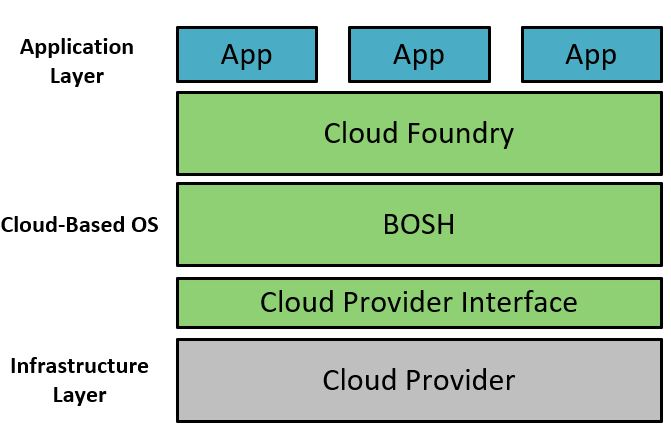
\includegraphics[width=10cm]{img/Cloud_Foundry_Layers.JPG}
		\caption[Einordnung Cloud Foundry Plattform]{Einordnung Cloud Foundry Plattform\\
			(\cite[Eigene Abbildung in Anlehnung an][S. 9]{Winn.2017})}
		\label{Cloud_Foundry_Layers}
	\end{center}
\end{figure}
\\
Wie aus der Grafik \ref{Cloud_Foundry_Layers} entnommen werden kann, bezeichnet Duncan Winn \ac{CF} als Teil eines Cloud basierten Betriebssystems. Dieses Betriebssystem verbirgt die eigentlichen Rechenressourcen, wie beispielsweise den virtuellen Speicher, den Arbeitsspeicher und die \acsp{CPU} und abstrahiert diese für den Endbenutzer in einfach verwendbare Dienste.\autocite[Vgl.][S. 8]{Winn.2017}\\
BOSH ist ein Open-Source Tool zur automatisierten Bereitstellung von Software und übernimmt das Management des Softwarelebenszyklus. Dabei wird mittels Manifestdateien die Provisionierung der virtuellen Maschinen, die Überwachung der Softwarekomponenten sowie die Anwendungsaktualisierungen mit \textbf{Zero-to-minimal Downtime} ermöglicht. \\
Die Erläuterung des Begriffs Zero-to-minimal Downtime erfolgt in Kapitel \ref{bewertung_cf}.\\
Mit Hilfe der einheitlich definierten Manifestdateien ermöglicht BOSH eine von der Infrastruktur unabhängige Beschreibung der Anwendungsbereitstellung.\autocite[Vgl.][S. 14-15]{Winn.2017}
\\
Zudem gehört \ac{CF} zur Cloud Foundry Foundation, welche eine Non-Profit-Organisation ist und ihre Produkte unter der freien Open-Source-Softwarelizenz Apache 2.0 veröffentlicht.\autocite[Vgl.][]{GitHubRepositoryCloudFoundry.2020}
%Laut Duncan Winn sind generelle cloud-native PaaS-Lösungen und somit auch \ac{CF} rechthaberisch. Das bedeutet, dass native Services der Plattform auf Best Practices basieren. Dadurch sind diese klar definiert und somit auch in ihrer Funktionsweise eingeschränkt. , wie beispielsweise die das Deployen von Microservices erfolgen soll. Dadurch soll eine einheitliche Benutzererfahrung unabhängig von der verwendeten Infrastruktur ermöglicht werden. \autocite[Vgl.][ 1. - The Opinionated Platform]{Winn.2017} \\

\section{Virtualisierung der Infrastruktur}
\subsection{Abgrenzung von Containern zu virtuellen Maschinen}
Generell verfolgen sowohl virtuelle Maschinen als auch Containertechnologien die Isolation einzelner Softwarekomponenten auf einem physischen Rechner. \autocite[Vgl.][S. 32-33]{Oggl.2018}
Dabei basieren laut Oliver Liebel fast alle Containertechnologien auf den Isolationsmechanismen des Linux Kernels, den \textbf{Linux Kernel Namespaces}. Dabei wird beispielsweise der PID-Namespace zur Kapselung der Container-Prozesse in eigenständige Root-Prozessbäume innerhalb des eigentlichen Host-Prozessbaumes verwendet.\autocite[Vgl.][S. 80-81]{Liebel.2019}
\\
\begin{figure}[h]
	\begin{center}
		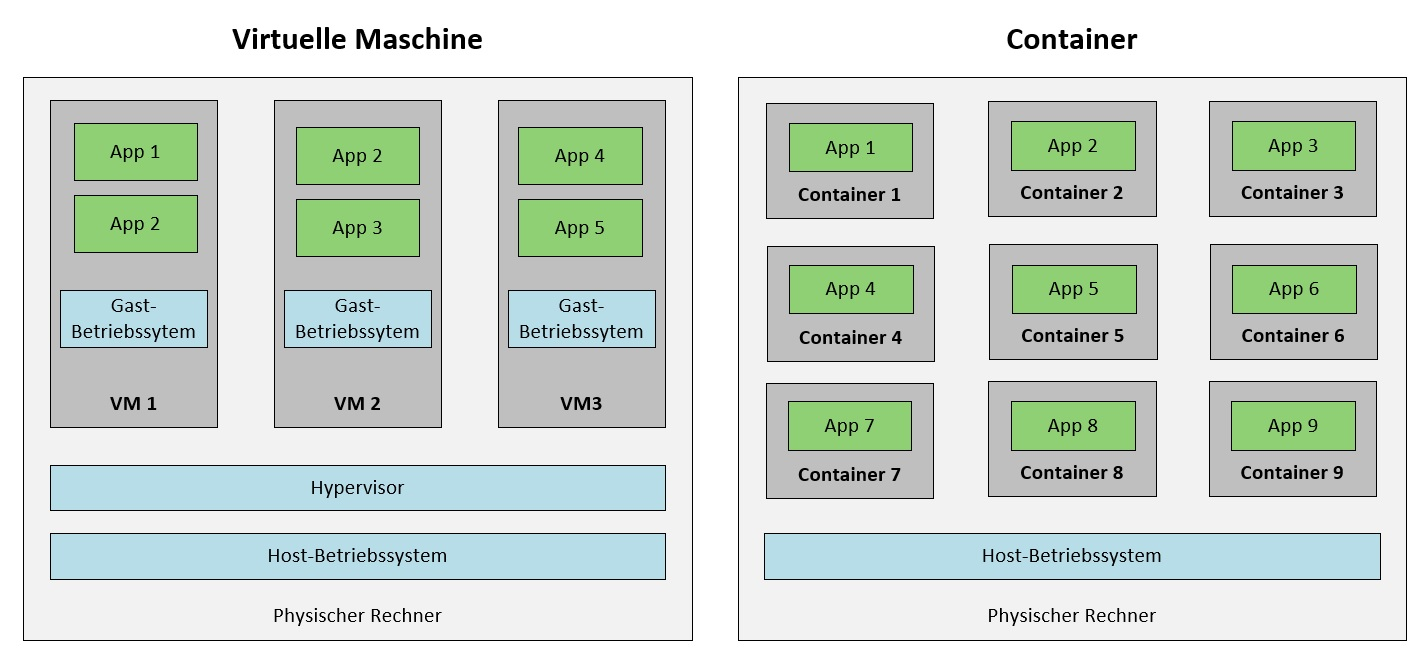
\includegraphics[width=16cm]{img/VM_vs_Container.JPG}
		\caption[Vergleich der Anwendungsbereitstellung mit \acsp{VM} und Containern]{Vergleich der Anwendungsbereitstellung mit \acsp{VM} und Containern\\
			(\cite[Eigene Abbildung in Anlehnung an][S.11]{Luksa.2018})}
		\label{Vergleich_VM_Container}
	\end{center}
\end{figure}
\newpage
Wie der Abbildung \ref{Vergleich_VM_Container} entnommen werden kann, haben Container im Vergleich zu \acsp{VM} kein eigenes Gast-Betriebssystem, sondern sind isolierte Prozesse, die auf dem Betriebssystem des zugrundeliegenden Hosts laufen. Dadurch können die bei \acsp{VM} benötigten Systemprozesse eingespart und Hardwareressourcen des physischen Rechners effektiver genutzt werden.\autocite[Vgl.][S. 10-12]{Luksa.2018}
\subsection{Containerisierung mit Docker}
\textbf{Docker} ist eine Container-Engine-Plattform und ermöglicht das ``Verpacken, Verteilen und Ausführen von Anwendungen`` \autocite[][S. 15]{Luksa.2018} mittels \textbf{Docker-Images}. Hierbei können die Images in einer zentralen \textbf{Image Registry} abgelegt werden. Dies ermöglicht die generelle Portierung der Container auf beliebige physische Rechner. Die einzige Voraussetzung hierfür ist, dass auf dem Host-Rechner die für das Docker Image vorgesehene Linux-Kernel Version läuft. Außerdem dienen die Images als Grundlage für die Container. Ein Container ist ein in einem ressourceneingeschränkten und isolierten Prozess des Host-Rechners ausgeführtes Image. \autocite[Vgl.][S. 14-15, 18]{Luksa.2018} Eine alternative Container Engine ist beispielsweise \textbf{cri-o}.\autocite[Vgl.][S. 79]{Liebel.2019}%Wie in Abbildung \ref{Container_Schichten_Architektur} zu sehen ist, gibt es neben Docker weitere alternative Container Engines, wie beispielsweise \textbf{cri-o}.\autocite[Vgl.][S. 108]{Liebel.2019} %Container-Engine, welche die \ac{OCI}-Standards erfüllt.\autocite[Vgl.][S. 108]{Liebel.2019}
\\
\begin{figure}[h]
	\begin{center}
		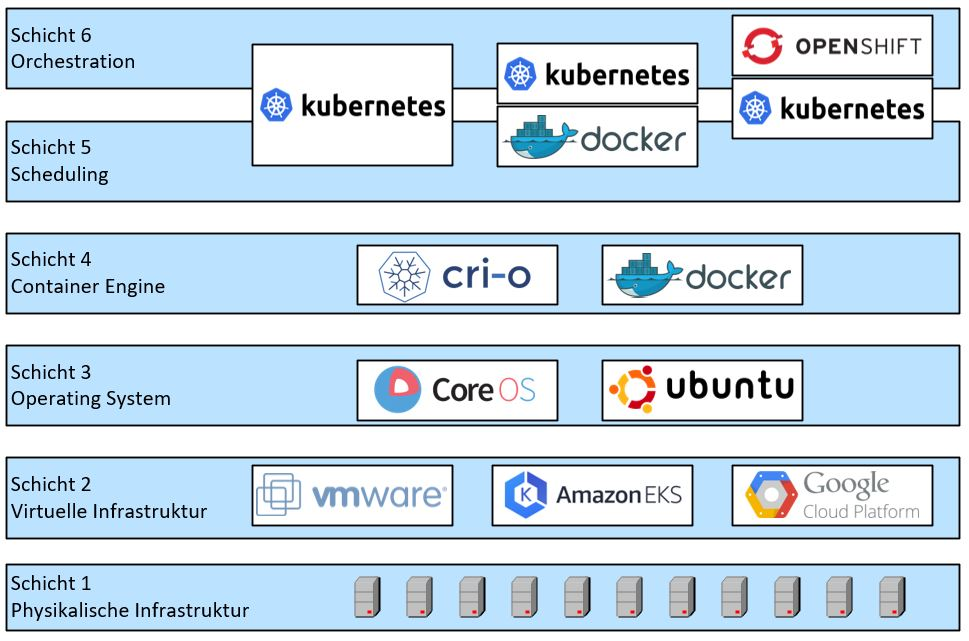
\includegraphics[width=14cm]{img/Container_Schichten_Architektur.JPG}
		\caption[Schichten einer containerbasierten Anwendungsbereitstellung]{Schichten einer containerbasierten Anwendungsbereitstellung\\
			(\cite[Eigene Abbildung in Anlehnung an][S.79]{Liebel.2019})}
		\label{Container_Schichten_Architektur}
	\end{center}
\end{figure}
\newpage
\section{Kubernetes}
\label{Kubernetes}
Kubernetes ist ein Open Source Softwaresystem zur Bereitstellung, Verwaltung und Orchestration von containerbasierten Anwendungen. Dabei wird die Hardwareschicht der Infrastruktur auf \textbf{Nodes} abstrahiert. Für das Entwicklungs- und Betriebsteam stellt sich das gesamte Infrastruktursystem, das physisch aus mehreren Rechnerclustern bestehen kann, als einziges virtuelles System dar. Dadurch sollen sich die Entwickler auf die eigentliche Anwendungsentwicklung konzentrieren können, indem sie auf die von Kubernetes bereitgestellten Dienste zurückgreifen können. Dies sind exemplarisch native Funktionen zur Lokalisierung von Services, automatischen Skalierung der Bereitstellungen, Lastenausgleichsfunktionen sowie Selbstheilungsmechanismen für die bereitgestellten Anwendungen.\autocite[Vgl.][S. 19-21]{Luksa.2018}\\
Bei der Kubernetes Plattform werden die Docker Container innerhalb von \textbf{Pods} bereitgestellt. Hierbei sind Pods generell die kleinste möglichste Recheneinheit, welche auf einem Kubernetes Cluster bereitgestellt werden kann und prinzipiell aus einem oder mehreren Containern bestehen können.
Zudem ist zu beachten, dass die in einem Pod ausgeführten Container im gleichen Kontext und dadurch mit einem geteilten Speicher und dem gleichen Netzwerk bereitgestellt werden. Damit teilen sich diese Container auch die gleiche \ac{IP}-Adresse und denselben Portraum.\\
Generell dienen die Kubernetes Pods als Abstraktionsmedium für die Bereitstellung von entweder eng oder lose gekoppelter Container. Dabei können eng gekoppelte Container innerhalb von einem Pod und lose gekoppelte Container in unterschiedlichen Pods bereitgestellt werden.\autocite[Vgl.][What is a Pod, Motivation for Pods]{KubernetesAuthors.20190806}
\subsection{Grundlagen des Kubernetes Clusters}
\label{Grundlagen_Kubernetes}
Generell besteht ein Kubernetes Cluster aus mindestens einer \textbf{Master Node} und einer \textbf{Worker Node}.\\
Dabei werden vereinfacht betrachtet die aus der Abbildung \ref{Grafik_Grundlagen_Kubernetes_Cluster} zu entnehmenden Komponenten auf der Master und Worker Node des Kubernetes Clusters bereitgestellt.
\\
\begin{figure}[h]
	\begin{center}
		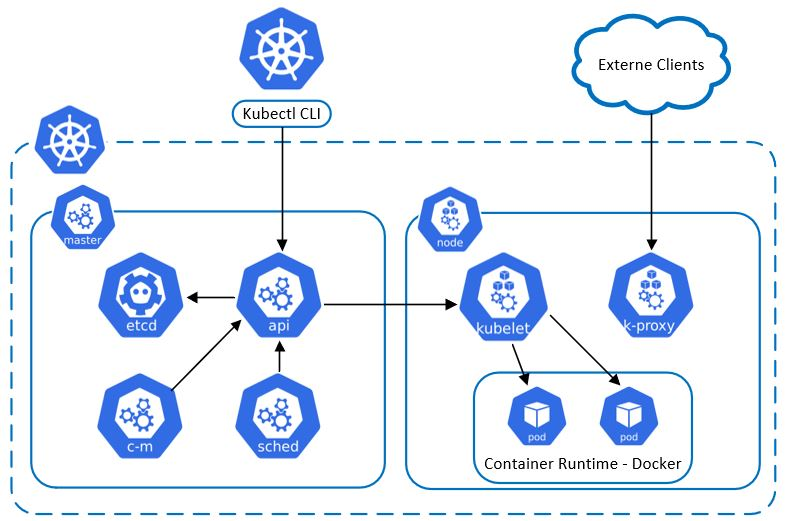
\includegraphics[width=16cm]{img/Kubernetes_Aufbau.JPG}
		\caption[Grundlagen Kubernetes Cluster]{Grundlagen Kubernetes Cluster \\
			(\cite[Eigene Abbildung in Anlehnung an][S.563]{Liebel.2019})}
		\label{Grafik_Grundlagen_Kubernetes_Cluster}
	\end{center}
\end{figure}
\\
\newpage
\begin{description}
	\item[API-Server] \hfill \\
	Der \ac{API}-Server ist die zentrale Administrationskomponente zur Verwaltung der Clusterobjekte. Dabei nimmt er alle Anfragen an, die zum Beispiel mit der \textbf{kubectl}-\ac{CLI} oder anderer \ac{GUI}-Lösungen an die \ac{REST}-Schnittstelle des \ac{API}-Servers gesendet werden. Anschließend validiert und verarbeitet er diese. Des Weiteren beinhaltet er alle Definitionen der Kubernetes-Objekte und stellt diese bereit.\autocite[Vgl.][S. 564-565]{Liebel.2019}
	\item[Controller Manager] \hfill \\
	Der Controller Manager übernimmt clusterweite Aufgaben, wie etwa die Sicherstellung der definierten Anzahl an replizierten Pods, die Überwachung der Worker Nodes sowie Gegenmaßnahmen bei einem Ausfall einer Node.\autocite[Vgl.][S. 565]{Liebel.2019}
	\item[Scheduler] \hfill \\
	Der Scheduler ist zuständig für die Zuweisung der Pod-Instanzen auf die Worker Nodes. Hierbei versucht er die aktuellen Workloads der Worker Nodes mittels deren freien Ressourcenkapazitäten zu optimieren. \autocite[Vgl.][S. 566]{Liebel.2019}
	\item[etcd] \hfill \\
	Der zentrale Key-Value Store etcd dient der persistenten Sicherung der Clusterkonfigurationen und des aktuellen Zustandes des \ac{API}-Servers.
	\item[kubelet] \hfill \\
	Der kubelet-Service fungiert als Kommunikations- und Steuerungsschnittstelle der \textbf{Worker Nodes} für den API-Server. Dabei sorgt er für die Bereitstellung der Kubernetes-Objekte in der lokalen Container Runtime, wie beispielsweise der Docker Engine.\autocite[Vgl.][S. 566-567]{Liebel.2019}
	\item[kube-proxy] \hfill \\
	Der kube-proxy-Dienst kümmert sich um die ``clusterweite, interne Bereitstellung von Services […] und um die Annahmen und Weiterleitung von der Außenwelt eingehender Requests``.\autocite[][S. 568]{Liebel.2019}
\end{description}
Die Erläuterung der einzelnen Kubernetes-Objekte, welche innerhalb des Prototyps verwendet und implementiert werden, erfolgt in den Kapiteln \ref{Konzeption_K8s_Cluster} und \ref{Umsetzung_K8s_Cluster}.\\
\subsection{Cluster Verwaltung mittels Gardener}
\label{Cluster_Verwaltung}
Das Gardener Projekt ist ein Open Source Projekt, welches das Ziel der kostenfreien Provisionierung von Kubernetes Clustern as-a-Service verfolgt. Dabei können die Kubernetes Cluster mit Hilfe von Gardener in wenigen Schritten konfiguriert und provisioniert werden. Für die weitere Verwaltung des Kubernetes Clusters bietet Gardener ein Dashboard sowie bereits vorinstallierte Lösungen und Tools welche beispielsweise für das Monitoring der Kubernetes Master Nodes eingesetzt werden können.\autocite[Vgl.][Gardener Dashboard]{GardenerAuthors.20200120}
\\
Zudem unterstützt Gardener den Multi-Cloud Ansatz dadurch, dass die benötigte Infrastruktur von unterschiedlichen \ac{IaaS}-Providern aus weltweit verteilten Regionen verwendet werden kann. Hierbei können zum aktuellen Zeitpunkt der vorliegenden Thesis die folgenden \ac{IaaS}-Provider eingesetzt werden: \ac{AWS}, Microsoft Azure Cloud, \ac{GCP}, Open Stack und Alibaba Cloud.\autocite[Vgl.][K8s Conformance Test Coverage]{GardenerAuthors.20200121} Die Auswahl der Regionen ist hierbei vom \ac{IaaS}-Provider abhängig.\\
Für die technische Bereitstellung des Kubernetes Clusters wird ausschließlich Rechenkapazität in Form von virtuellen Maschineninstanzen und persistentem Speicherplatz benötigt.\\
Des Weiteren ermöglicht Gardener eine automatische Skalierung der für die Nodes verwendeten \acsp{VM}.
\newpage 
Dabei definiert der Clusteradministrator den Maschinentyp der virtuellen Recheninstanzen, die Art des persistenten Speichermediums sowie die minimale und maximale Anzahl an Recheninstanzen. Die horizontale Skalierung wird anschließend automatisch abhängig vom Rechenkapazitätsbedarf des Kubernetes Clusters durchgeführt. \\
Außerdem stellt Gardener verglichen mit anderen Cluster-as-a-Service-Anbieter homogene und nicht proprietäre Kubernetes Cluster zur Verfügung. Das bedeutet, dass Gardener durch die Open Source Community versucht einen offenen Standard für die Provisionierung eines Kubernetes Clusters zu etablieren. Allerdings unterstützt Gardener zum Zeitpunkt der vorliegenden Thesis ausschließlich die Container Engine Docker.\\
%Anmerkung: Quelle einfügen!
Eine weitere Funktion, die zur generellen Senkung der Betriebskosten des Clusters genutzt werden kann, ist die Konfiguration des Cluster-Lifecycles. Dabei kann definiert werden, an welchen Tagen und zu welcher Uhrzeit das Cluster automatisch gestartet und wieder heruntergefahren werden soll.\autocite[Vgl.][Configuration]{GardenerAuthors.20200120}
\\
\section{SAP Subscription Billing}
\subsection{Fachliches Anwendungsgebiet}
SAP Subscription Billing ist eine \ac{SaaS}-Lösung zur Automatisierung und Optimierung der Abrechnungs- und Bestellprozesse. Dadurch sollen besonders innovative Geschäftsmodelle, die auf wiederkehrenden Zahlungen oder einer nutzungsabhängigen Gebührenberechnung basieren, schnell geplant, modelliert und umgesetzt werden können.\\ 
Insbesondere durch das nutzungsbasierte Abrechnungsmodell ermöglicht die Softwarelösung ihren Kunden beliebige ``as-a-Service``-Szenarien zu bedienen.
Hierbei sind die von einem Unternehmen angebotenen Produkte und die dafür definierten Tarifpläne der Kern der Softwarelösung. Dadurch können mit Hilfe des effektiven Verbrauchs der Kunden und den für das entsprechende Produkt definierten Tarifplänen die nutzungsabhängige Berechnung der Gebühren durchgeführt werden.\autocite[Vgl.][SAP Subscription Billing]{SAPSEodereinSAPKonzernunternehmen.2019}
\\
\newpage
\subsection{Technische Grundlagen}
Aus technischer Sicht ist SAP Subscription Billing laut der deutschsprachigen SAP Anwendergruppe eine mandantenfähige Softwarelösung, die für den Endanwender in der Public Cloud bereitgestellt wird. Generell basiert die Softwareösung auf einer Microservice-Architektur, welche mittels der \ac{CF}-Umgebung der \ac{SCP} bereitgestellt wird. Zudem bietet die Lösung offene \ac{API}-Schnittstellen an, welche zur Integration in eigene Infrastruktur-Landschaften genutzt werden können. Alternativ ist die Lösung mittels des zentralen Einstiegspunktes \url{https://revenue.cloud.sap} auch als Webanwendung mit einer grafischen Benutzeroberfläche erreichbar. \autocite[Vgl.][]{DeutschsprachigeSAPAnwendergruppe.2018}\\
Des Weiteren wurde die \ac{SaaS}-Lösung mit den zur Verfügung stehenden \acsp{API}\footnote{\ac{API} Hub SAP Subscription Billing: \url{https://api.sap.com/package/SAPHybrisRevenueCloud?section=Artifacts}} in weitere SAP Lösungen, wie beispielsweise SAP S/4HANA Cloud oder SAP Commerce Cloud integriert.\autocite[Vgl.][SAP Subscription Billing - Integration]{SAPSEodereinSAPKonzernunternehmen.20200205} Die ausführliche Erläuterung des technischen Aufbaus der \ac{SaaS}-Lösung erfolgt in Kapitel \ref{technischer_aufbau_cf}.\\




% !TEX root =  master.tex
\chapter{Formulierung der Vergleichsmetrik für den Infrastrukturvergleich}
\label{merkmale}
Die folgenden Unterkapitel beinhalten die Formulierung der Merkmale für den Vergleich der Plattformen \ac{CF} und Kubernetes und der dabei verwendeten Methodik. Des Weiteren erfolgt die Kategorisierung der Vergleichsmerkmale sowie die Erläuterung der Untersuchungsvorgehensweise. Abschließend wird die Gewichtung der definierten Merkmale anhand der für eine Portierung ausschlaggebenden Kriterien des Infrastruktur-Teams durchgeführt.
\section{Vorgehensweise zur Ermittlung der Vergleichsmetrik}
Die Formulierung der Vergleichsmerkmale wurde durch die Eindrücke und Erfahrungen durchgeführt, welche im Rahmen dieser Thesis stattgefundenen praktischen Mitarbeit im Projekt SAP Subscription Billing gesammelt wurden. Zudem basieren sie auf der \ac{ISO}-Norm 25010, welche ein Modell für die allgemeinen Qualitätsanforderungen von Software definiert.\footnote{\ac{ISO}-Norm 25010: \url{https://www.iso.org/standard/35733.html}}
Des Weiteren wurden diese in Zusammenarbeit mit den Architekten des Infrastruktur-Teams aus dem SAP Subscription Billing Projekt evaluiert und an die projektinternen Interessen und die ausschlaggebenden Kriterien, die zur Rechtfertigung der Portierung der \ac{SaaS}-Lösung verwendet werden können, angepasst.
\section{Kategorisierung der Merkmale}
Die Merkmale können mittels der Unterscheidung in Vergleichsmerkmale, die entweder funktionale oder nicht funktionale Anforderungen beinhalten, kategorisiert werden. Dabei handelt es sich bei funktionalen Anforderungen um Funktionen, welche von der Plattform unterstützt oder nativ angeboten werden. Die nicht funktionalen Anforderungen belaufen sich hierbei auf allgemeine Qualitätsattribute der Software.\\
\\\\
Innerhalb der praktischen Arbeit der vorliegenden Thesis wurden folgende funktionale Vergleichsmerkmale untersucht: zusätzlich benötigte Infrastruktur-Services und die Funktionalitäten für das Monitoring und das Management der Logdateien der Microservices.\\
Als nicht funktionale Vergleichsmerkmale wurden die folgenden Merkmale betrachtet und ausgewertet: Performance, monatliche Kosten, Sicherheit, Verfügbarkeit der Plattform, Mechanismen zur Skalierung, Konfigurierbarkeit, Erweiterbarkeit, benötigte Einarbeitungszeit und die Portierbarkeit der Bereitstellung der Anwendung.

\section{Erläuterung der Qualitätsattribute und der Untersuchungsvorgehensweise}
\label{kapitel_merkmale_vorgehensweise}
\begin{description}
	\item[Performance] \hfill \\
	Die Untersuchung der Performance der beiden Plattformen wird mittels der Messung der durchschnittlichen Antwortzeit der \ac{HTTPS}-Anfragen, der Gesamtanzahl an beantworteten Anfragen und dem Durchsatz an Anfragen pro Sekunde durchgeführt. Diese Tests werden mit Hilfe des Apache JMeter Tools ausgeführt.\footnote{Weitere Informationen zu JMeter: \url{https://jmeter.apache.org/}} Dabei werden mit mehreren Threads parallelisierte Anfragen, welche keine Kommunikation zwischen dem Microservice und der Datenbank benötigen, an die \ac{API}-Schnittstelle eines bereitgestellten Microservices gesendet. Dieser wird aus Gründen der Vergleichbarkeit mit den gleichen Rechenkapazitäten und der übereinstimmenden Anzahl an Replikaten jeweils auf der \ac{CF} und dem Kubernetes Cluster bereitgestellt.
	Dabei werden pro Plattform fünf Tests mit einer Dauer von jeweils fünf Minuten für jede unterschiedliche Testkonfiguration durchgeführt. Die Testkonfigurationen unterscheiden sich in der Anzahl der gleichzeitigen Threads. Hierbei sollen jeweils drei Konfigurationen mit 100, 150 und 200 Threads ausgewertet werden.
	\item[Kosten] \hfill \\
	Bei der Betrachtung der Kosten wird eine Eingrenzung auf die für die Anwendungsumgebung anfallenden Kosten vorgenommen. Dies bedeutet, dass der Kostenvergleich mit den Kosten pro \ac{GB} \ac{RAM} der Anwendungsumgebung	durchgeführt wird. Zum aktuellen Zeitpunkt der vorliegenden Thesis sind die 15 Microservices der \ac{SaaS}-Lösung mit jeweils einem \ac{GB} \ac{RAM} und zwei Instanzen auf der \ac{CF} bereitgestellt. Eine Ausnahme ist nur ein rechenintensiver Microservice, welcher zwei \ac{GB} \ac{RAM} zur Verfügung hat. Somit werden insgesamt 34 \ac{GB} \ac{RAM} als Vergleichswert für die Kosten der beiden Plattformen angenommen. Außerdem wird der weitere Wert von 780 \ac{GB} \ac{RAM} betrachtet, der aus projektinternen Berechnungen aller für das Projekt benötigten Rechenressourcen hervorgeht. Dieser Wert setzt sich aus den verschiedenen Landschaften zusammen, welche für die Trennung der Entwicklungs-, Test- und Produktivumgebung dienen.\\
	Jedoch sollte hierbei beachtet werden, dass diese Untersuchungsvorgehensweise ausschließlich einen Teil der eigentlich repräsentativeren \ac{TCO} betrachtet. Der Vergleich der gesamten \ac{TCO} ist aufgrund des eingeschränkten zeitlichen Rahmens der Thesis und durch die unklaren Informationen innerhalb des SAP Subscription Billing Projektes nicht möglich.
	\item[Sicherheit] \hfill \\
	Die Sicherheit wird mit Hilfe der theoretischen Konzepte der Anwendungsbereitstellung der beiden Plattformen untersucht. Hierbei spielen besonders die externe Verfügbarkeit der Anwendungen und und die Konzepte für die Umsetzung von Zugriffsberechtigungen eine wichtige Rolle. Des Weiteren werden die Mechanismen zur generellen Absicherung der Kommunikation der Microservices untereinander betrachtet. Hierbei soll auch die Möglichkeit einer ungewollten Kommunikation von Microservices, welche in unterschiedlichen Landschaften bereitgestellt sind, untersucht werden. 
	\item[Verfügbarkeit] \hfill \\
	Die Verfügbarkeit kann aufgrund fehlender Kennzahlen und Informationen bezüglich der effektiven Verfügbarkeit der beiden Plattformen und der zusätzlichen Abhängigkeit der zugrundeliegenden Infrastruktur und den eingesetzten Datenbanken ausschließlich anhand der \acsp{SLA} verglichen werden. Zudem werden die Funktionalitäten zur Sicherstellung der Verfügbarkeit untersucht und ausgewertet.
	\item[Skalierbarkeit] \hfill \\
	Der Vergleich der Skalierbarkeit wird mit Hilfe der Auswertung der Mechanismen für die automatische Skalierung der bereitgestellten Anwendung durchgeführt. Diese sollte abhängig von der sich dynamisch ändernden Auslastung der Infrastruktur und der Anwendung sein. Zudem wird hierbei in die vertikale und horizontale Dimension der Skalierbarkeit sowie den möglichen Ebenen der Skalierung unterschiedenen.
	\item[Konfigurierbarkeit] \hfill \\
	Die Auswertung der Konfigurierbarkeit erfolgt seitens der \ac{CF} mittels der Expertise der Softwareentwickler, die bereits seit mehreren Jahren täglich mit der \ac{CF}-Plattform arbeiten. Außerdem fließen besonders die praktischen Erfahrungen, welche im Rahmen dieser Thesis bei der Umsetzung der Portierung der \ac{SaaS}-Lösung auf ein Kubernetes Cluster gesammelt wurden, in die Auswertung der Konfigurierbarkeit von Kubernetes mit ein. 
	\item[Erweiterbarkeit] \hfill \\
	Zur Evaluation der Erweiterbarkeit dienen die von den Plattformen unterstützten Strategien für die Aktualisierung einer bereitgestellten Anwendung. Des Weiteren wird hierbei auf die Möglichkeit des sogenannten \textbf{Zero-Downtime-Deployments} geachtet. Dies zielt auf eine unterbrechungsfreie Aktualisierung der bereitgestellten Anwendung ab.
	\item[Einarbeitungszeit] \hfill \\
	Die Auswertung der benötigten Einarbeitungszeit geschieht, wie auch die Betrachtung der Konfigurierbarkeit, basierend auf den gesammelten praktischen Erfahrungen. Hierbei spielt besonders das theoretische und praktische Wissen, das für eine erste Bereitstellung einer Anwendung auf der Plattform benötigt wird, eine wichtige Rolle.
	\item[Portierbarkeit] \hfill \\
	Das Merkmal der Portierbarkeit dient zur Betrachtung der Möglichkeiten eines Wechsels des \ac{IaaS}-Providers. Zudem wird die Unterstützung von \textbf{Multi-Cloud-Szenarien} und der Anwendungsbereitstellung in unterschiedlichen Regionen ausgewertet. Die spezifische Erläuterung des Multi-Cloud-Szenarios findet in Kapitel \ref{bewertung_cf} statt.
	\item[Infrastruktur-Services] \hfill \\
	Mit dem Merkmal Infrastruktur-Services werden zusätzlich Microservices und weitere Infrastruktur-Komponenten, welche zum Abdecken von nicht von der Plattform nativ bereitgestellten Funktionalitäten benötigt werden, dargestellt. Dabei wird bei der prototypischen Bereitstellung der Software auf dem Kubernetes Cluster die Notwendigkeit ausgewählter Infrastruktur-Services untersucht, welche bei der aktuellen Infrastrukturlösung mit \ac{CF} eingesetzt werden.   
	\item[Monitoring und Logging] \hfill \\
	Im Rahmen der Untersuchung der Möglichkeiten für das Monitoring der bereitgestellten Anwendung und das zentrale Verwalten der Logdateien sollen die verwendeten Tools der aktuell auf der \ac{CF} basierenden Infrastrukturlösung auch auf dem Kubernetes Cluster implementiert und ausgewertet werden. Die hierbei eingesetzten Tools werden in Kapitel \ref{bewertung_cf} vorgestellt. Des Weiteren werden die hierfür anfallenden Kosten sowie der Aufwand für den Betrieb der Tools betrachtet.
\end{description}
\newpage
\section{Gewichtung der Vergleichsmerkmale}
\label{gewichtung_merkmale}
Da die vorliegende Thesis auf die Evaluation der beiden Plattformen für das Infrastruktur-Team des SAP Subscription Billing Projektes abzielt, erfolgt auch die Gewichtung der Vergleichsmerkmale anhand der für das Infrastruktur-Team ausschlaggebenden Kriterien.\\ 
Dieses ist unter anderem für den täglichen Betrieb aller Systemlandschaften verantwortlich, welche für den produktiven Betrieb und die Weiterentwicklung der \ac{SaaS}-Lösung genutzt werden. Des Weiteren führt das Infrastruktur-Team die täglich stattfindende Aktualisierung der bereitgestellten Softwarelösung auf allen vorhandenen Systemlandschaften durch.\\ 
Innerhalb der praktischen Mitarbeit im Infrastruktur-Team wurde festgestellt, dass für den produktiven Betrieb der \ac{SaaS}-Lösung besonders die Verfügbarkeit der eingesetzten Plattform, deren Mechanismen zur Skalierung und die generell unterstützen Sicherheitskonzepte ausschlaggebend sind. Außerdem sind auch die Konfigurierbarkeit, die Möglichkeiten für das Monitoring und Logging sowie die Erweiterbarkeit der Softwarelösung besonders relevant. Dabei begründet sich beispielsweise die stärkere Gewichtung der Erweiterbarkeit durch die täglich durchgeführte Aktualisierung der Anwendungen, welche aufgrund der Häufigkeit automatisiert und ohne Unterbrechung durchgeführt werden muss.\\
\\
Deshalb sind die zuvor genannten Qualitätsmerkmale für die wissenschaftliche Untersuchung der vorliegenden Thesis ausschlaggebend und werden innerhalb des Vergleichs der beiden Plattformen stärker gewichtet.
\begin{comment}
	Aus der Sicht des Anwenders der Software wird die Gewichtung der Merkmale basierend auf den Ergebnissen der Forschung von Claus-Peter H. Ernst und Franz Rothlauf, welche im Jahr 2012 die potentiellen Erfolgsfaktoren von \ac{SaaS}-Unternehmen mittels des damaligen Forschungsstandes gesammelt und zusammengefasst haben, durchgeführt.\\
	Laut Claus-Peter H. Ernst und Franz Rothlauf sind aus Sicht des Anwenders primär die für die Benutzung des \ac{SaaS}-Angebots anfallenden Kosten sowie die Sicherheit der Daten ausschlaggebend.\autocite[Vgl.][S. 5]{Ernst.2012}
	Jedoch sollte dies aufgrund der Weiterentwicklungen innerhalb des vergangenen Jahren nicht als vollumfängliches Ergebnis gesehen werden, da besonders die Verfügbarkeit auch für den Anwender der \ac{SaaS}-Lösung wesentlich ist.\\
	\\
	Insgesamt kann durch die zuvor aufgezeigten Interessengruppen und deren ausschlaggebenden Qualitätsmerkmale für die Auswahl einer Plattform zur Bereitstellung einer \ac{SaaS}-Lösung die stärkere Gewichtung der zuvor aufgezählten Merkmale für die wissenschaftliche Untersuchung der vorliegenden Thesis angenommen werden. 
\end{comment}

 



% !TEX root =  master.tex
\chapter{Analyse der Infrastrukturlösung von SAP Subscription Billing}
\label{Kapitel_Infrastruktur_CF}
Die folgenden beiden Unterkapitel beinhalten den Überblick des technischen Aufbaus der SAP Subscription Billing \ac{SaaS}-Lösung auf der \ac{CF} und die Erläuterung der für die prototypische Portierung relevanten Komponenten. Zudem erfolgt die Evaluation der \ac{CF}-Plattform mittels der in Kapitel \ref{kapitel_merkmale_vorgehensweise} definierten Merkmale und Untersuchungsvorgehensweise.
\section{Technischer Aufbau}
\label{technischer_aufbau_cf}
Die Übersicht des technischen Aufbaus der Infrastrukturlösung ist aus der Grafik \ref{grafik_technischer_aufbau_cf} zu entnehmen.
\begin{figure}[h]
	\begin{center}
		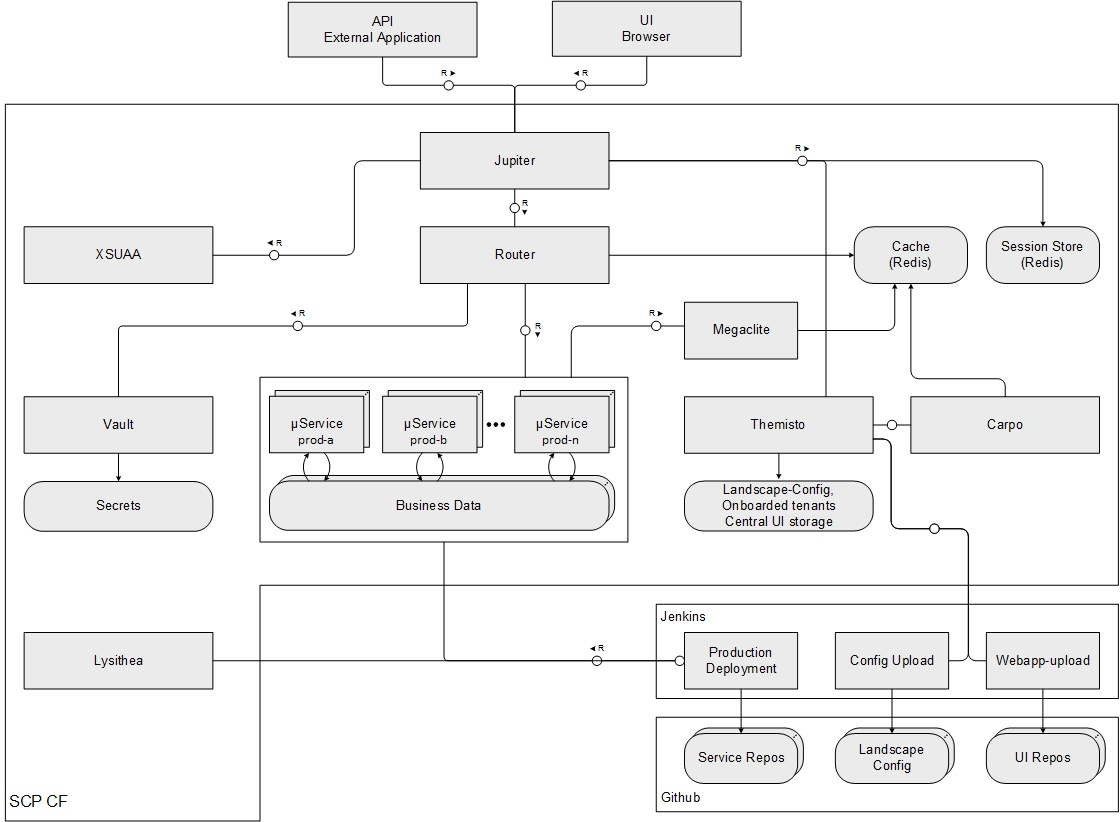
\includegraphics[width=16cm]{img/cf_infrastruktur.JPG}
		\caption[Überblick Infrastrukturlösung SAP Subscription Billing]{Überblick Infrastrukturlösung SAP Subscription Billing\\ Abbildung stammt aus dem projektinternen Wiki}
		\label{grafik_technischer_aufbau_cf}
	\end{center}
\end{figure}
\\
Der \textbf{Jupiter} ist der zentrale Einstiegspunkt sowohl für die Anfragen, welche direkt an die \ac{API}-Endpunkte geschickt werden, als auch für die aus der Webanwendung stammenden Anfragen. Zudem führt er mittels des \ac{XSUAA} der \ac{SCP} die Authentifikation der externen Anfragen durch.
Der \ac{XSUAA}-Dienst basiert auf dem Standardprotokoll \textbf{OAuth} 2.0, welches für die Authentifikation der Clients genutzt werden kann. Dadurch eignet sich dieser Dienst besonders für die Umsetzung von Berechtigungskonzepten einer mandantenfähigen Softwarelösungen.\autocite[Vgl.][]{SAPSEodereinSAPKonzernunternehmen.2020}%\footnote{Weitere Informationen zu \ac{XSUAA}: \url{https://help.sap.com/viewer/65de2977205c403bbc107264b8eccf4b/Cloud/en-US/ea0281368f11472b8d2b145a2a28666c.html}}\\
Nach der erfolgreichen Authentifizierung führt der \textbf{Landscape-Router} das Routing der Anfrage an die entsprechende \ac{REST}-Schnittstelle der Microservices durch. Dabei wird mit Hilfe des Mandanten, welcher jeweils einer Landschaft, wie etwa der Test- oder auch der Produktiv-Landschaft zugeordnet ist, die Weiterleitung zur entsprechenden \ac{CF}-Landschaft durchgeführt. Dabei ist jeder Mandant genau für eine \ac{CF}-Landschaft einer geografischen Region berechtigt.\\
\textbf{Vault} ist ein vom Unternehmen Hashicorp angebotener Dienst zur zentralen Speicherung und Verwaltung von Credentials, Tokens und Zertifikaten. Dieser kommt aktuell zum Beispiel für die gegenseitige Authentifizierung der Microservices zum Einsatz.\footnote{Weitere Informationen zu Vault: \url{https://www.vaultproject.io/}}\\
\textbf{Themisto} ist der zentrale Speicherort sowohl für die \ac{GUI}-Vektoren als auch die statischen Dateien der Webanwendung. Vektoren kommen innerhalb des SAP Subscription Billing Projektes als zentrales Konzept zur Versionsverwaltung der einzelnen Microservices und der Komponenten der Webanwendung zum Einsatz. Dabei beschreibt ein \ac{GUI}-Vektor immer einen Stand der aktuell bereitgestellten Versionen der Komponenten der Webanwendung. Generell ist ein Vektor immer genau einer \ac{CF}-Landschaft zugeordnet. Des Weiteren inkludiert Themisto einen Webserver, der für die Bereitstellung der Webanwendung zuständig ist.\\
Generell entspricht \textbf{Lysithea} dem Zweck von Themisto. Allerdings verwaltet und speichert Lysithea die Microservice-Vektoren, welche funktional den \ac{GUI}-Vektoren entsprechen und zur Versionsverwaltung der Microservice Artefakte dienen.\\  
Der \textbf{Jenkins-Server} wird zur Automatisierung des Bereitstellungsprozesses der Anwendung eingesetzt. Dabei wird das Kompilieren, Testen und die eigentliche Bereitstellung mit Hilfe einer \ac{CI}/\ac{CD}-Pipeline durchgeführt. Diese Pipeline wird deklarativ mittels nacheinander ausgeführten Abarbeitungsschritten definiert. Der Jenkins-Server greift direkt auf die Git-Repositories zu, welche den Sourcecode der Microservices beinhalten. Dabei kann zum Beispiel bei jeder Aktualisierung einer Datei des Repositories die automatische Ausführung der für dieses Git-Repository hinterlegten Pipeline festgelegt werden.\footnote{Weitere Informationen zu Jenkins: \url{https://jenkins.io/doc/}}\\ 
\\
\newpage
Die Infrastrukur-Komponente \textbf{Landscape Config} verwaltet die Zuordnung der Vektoren zu den verschiedenen \ac{CF}-Landschaften. Zudem definiert sie das Berechtigungskonzept, welches beispielsweise ausschließlich festgelegte Personengruppen für die Aktualisierung der auf den Produktivlandschaften bereitgestellten Anwendungen berechtigt.\\
\\
Die weiteren Komponenten der Infrastrukturlösung können aufgrund der vereinfachten Erläuterung, sowie nicht benötigtem Wissen für das Verständnis der vorliegenden Thesis vernachlässigt werden.\\
Generell sind der Jenkins-Server und die Git-Repositories die einzelnen Komponenten, die außerhalb der \ac{CFAR} bereitgestellt sind. Die \ac{CFAR} ist die Anwendungsumgebung, in der die Anwendungen innerhalb der \ac{CF} bereitgestellt werden. Die für die Microservice benötigten Datenbanken sind in der Grafik \ref{grafik_technischer_aufbau_cf} vereinfacht und in der Komponente Business-Data dargestellt.\\
Eine detaillierte Darstellung aller Microservices und den hierbei verwendeten Datenbankinstanzen ist im Anhang in Kapitel \ref{grafik_ssb_microservices} zu finden.

\section{Bewertung der \acl{CF} Plattform}
\label{bewertung_cf}
\begin{description}
	\item[Performance] \hfill \\
	Bei der Untersuchung der Performance der auf der \ac{CF} bereitgestellten Anwendungen wurde mit Hilfe des JMeter Tools und einer beispielhaften \ac{HTTPS}-Anfrage an einen bereitgestellten Microservice die in der Tabelle \ref{tabelle_ergebnisse_performance_cf} dargestellten Durchschnittswerte ermittelt. Dabei wurde der Rater-Microservice verwendet, welcher fachlich in Kapitel \ref{Konzeption_Auswahl_Microservices} erläutert wird.\\
	\begin{table}[ht]
		\centering
		\begin{tabular}[h]{c|c|c|c}
			Threads & Anzahl Anfragen & Antwortzeit pro Anfrage & Durchsatz pro Sekunde \\
			\hline
			100 & 360373,8 & 81,2 ms & 1200,20
			\\
			\hline
			150 & 365360 & 120.4 ms	& 1217,30
			\\
			\hline
			200 & 364580.8 & 161,2 ms & 1214,78
			\\
		\end{tabular}\\
		\caption{Ergebnisse Performancetests: \acl{CF} in Frankfurt}
		\label{tabelle_ergebnisse_performance_cf}
	\end{table}
	\\
	Die vollständige Übersicht der einzelnen Testläufe mit weiteren Variablen ist im Anhang in Kapitel \ref{section_performance_test_cf} zu finden. Außerdem werden dort auch weitere Informationen bezüglich des genaues Testsetups erläutert.
	\item[Kosten] \hfill \\
	Wie bereits in Kapitel \ref{kapitel_merkmale_vorgehensweise} beschrieben, werden für den Kostenvergleich der beiden Plattformen die Vergleichswerte von 34 und 780 \ac{GB} \ac{RAM} herangezogen.\\
	Es ist zu beachten, dass es sich bei den Kosten der von der \ac{SCP} angebotenen \ac{CF}-Umgebung um das interne Kostenverrechnungsmodell für das SAP Subscription Billing Projekt handelt. Diese Betrachtung wurde gemacht, da für das Projekt SAP Subscription Billing dieses Verrechnungsmodell relevant ist.\\
	Im Fall von SAP Subscription Billing basiert die \ac{SCP} auf der Infrastruktur von \ac{AWS} und wird in der Region \textbf{EU10} in Frankfurt betrieben. \\
	Zudem ist zu berücksichtigen, dass der Application Runtime-Service für die \ac{CF} in drei unterschiedliche Preisklassen, abhängig von der gesamten Anzahl an gebuchten \ac{GB}, unterteilt wird. Für diesen Kostenvergleich ist die Preisklasse 1 mit monatlichen Kosten von 18,24 EUR pro \ac{GB} \ac{RAM} und die Preisklasse 2 relevant, welche für eine Gesamtanzahl an 100 \ac{GB} bis 1000 \ac{GB} \ac{RAM} gilt. Hierbei fallen monatliche Kosten in Höhe von 13,57 EUR pro \ac{GB} \ac{RAM} an.\\
	\\
	$\textrm{Monatliche Kosten 34 \ac{GB} \ac{RAM}} = 34 \cdot 18,24 \textrm{\euro} = 620,16 \textrm{\euro}\\
		\textrm{Monatliche Kosten 780 \ac{GB} \ac{RAM}} = 780 \cdot 13,57 \textrm{\euro} = 10.584,60 \textrm{\euro}$
	\\
	\\
	Dabei ist zu berücksichtigen, dass es sich im Fall des SAP Subscription Billing Projektes um feste monatliche Abonnementkosten handelt und hierbei keine nutzungsabhängige Berechnung der Kosten durchgeführt wird.
	\item[Sicherheit] \hfill \\
	Die Sicherheit der \ac{CF}-Plattform basiert auf den Sicherheitsaspekten der \ac{CFAR}. Diese sieht eine Bereitstellung der Anwendungen auf \acsp{VM} innerhalb eines privaten \ac{VLAN} vor. Der externe Zugriff auf die bereitgestellten Anwendungen erfolgt mittels eines extern erreichbaren Load Balancers.
	Der Load Balancer nimmt die auf dem \ac{HTTPS}-Protokoll basierenden Anfragen an und routet sie nach der erfolgreichen Authentifikation und Autorisierung durch den \ac{XSUAA}-Dienst und den Routern der \ac{CFAR} an den entsprechenden Endpunkt des Microservice weiter.\\
	Besonders positiv ist hierbei die abgeschirmte Bereitstellung der eigentlichen Microservices in einem privaten \ac{VLAN}. Zudem ist die Verwendung der \ac{TLS}-Verschlüsselung für die Kommunikation des extern verfügbaren Load Balancers als positiv zu werten.\autocite[Vgl.][System Boundaries and Access]{CloudFoundryFoundation.20191217}\\
	Jedoch zeigte sich vor allem bei der praktischen Verwendung der \ac{CF} Plattform, dass bei der Bereitstellung einer Anwendung standardmäßig eine extern verfügbare Adresse, bestehend aus dem Hostnamen und dem Domainnamen generiert wird. 
	\newpage
	Somit ist es bei der Verwendung der \ac{CF} innerhalb des SAP Subscription Billing Projektes nicht möglich einen Microservice, welcher keinen externen Zugriff benötigt, ausschließlich im privaten \ac{VLAN} der \ac{CFAR} zur Verfügung zu stellen. 
	Ein Beispiel ist die öffentlich verfügbare \ac{URL} des Rater-Microservices: \url{https://rater.cfapps.eu10.hana.ondemand.com}
	\\
	Eine Absicherung gegen ungewollte externe Zugriffe ist im SAP Subscription Billing Projektes ausschließlich seitens des Einsatzes der \ac{RBAC} möglich. 
	Diese basiert auf dem OAuth 2.0-Protokoll und sieht die Authentifikation des Benutzers durch die Angabe des Mandanten, des Benutzernamens und des Passworts vor. 
	\\
	Eine virtuelle Trennung nicht zusammengehörender Anwendungen ist bei der \ac{CF} mit Hilfe der Verwendung von \textbf{Orgs} und \textbf{Spaces} möglich. Hierbei können einer Org mehrere Spaces zugeordnet sein. Damit lässt sich beispielsweise die Trennung von Entwicklungs- und Produktivlandschaften ermöglichen.\\ 
	Allerdings ist zu beachten, dass dadurch nicht sichergestellt ist, dass keine ungewollte Kommunikation zwischen Microservices aus unterschiedlichen Spaces stattfinden kann. Da, wie zuvor erläutert, jeder Microservice automatisch eine externe \ac{URL} zur Verfügung gestellt bekommt, können diese auch für die nicht vorgesehene Kommunikation der Microservices aus unterschiedlichen \ac{CF}-Spaces genutzt werden.\autocite[Vgl.][Isolation Segments]{CloudFoundryFoundation.20191217}
	\item[Verfügbarkeit] \hfill \\
	Wie bereits in Kapitel \ref{kapitel_merkmale_vorgehensweise} erläutert, erfolgt die Evaluation der Verfügbarkeit ausschließlich anhand den angegeben \acsp{SLA} und den Mechanismen zur Sicherstellung der Verfügbarkeit.\\
	Hierfür gibt SAP laut des \acsp{SLA} zum aktuellen Zeitpunkt der Thesis eine Verfügbarkeit der \ac{CF}-Umgebung auf der \ac{SCP} von mindestens 99,5\% pro Monat an.\\
	Jedoch ist zu beachten, dass die SAP sich hierbei einen wöchentlichen vierstündigen Zeitraum als Wartungsfenster einräumt. Dieser ist abhängig von der Region und beginnt beispielsweise für Europa jeden Samstag ab 23:00 Uhr. Bei der Berechnung der effektiven Verfügbarkeit wird der festgelegte Wartungszeitraum jedoch berücksichtigt und von der Gesamtminutenanzahl im Monat abgezogen.\autocite[Vgl.][Systemverfügbarkeit]{SAPSEodereinSAPKonzernunternehmen.2019}\\
	%Die Berechnung der effektiven Verfügbarkeit berechnet sich wie folgt: \\
	%\begin{eqnarray}
	%\textrm{Systemverfügbarkeit} = (\textrm{(Gesamtminuten im Monat – Ausgeschlossene Ausfallzeit - Ausfallzeit)}
	%\end{eqnarray}
	%	-	Systemverfügbarkeit =((Gesamtminuten im Monat – Ausgeschlossene Ausfallzeit - Ausfallzeit) / (Gesamtminuten im Monat - Ausgeschlossene Ausfallszeit))∗100
	Bezüglich der nativen Mechanismen der Plattform zur Sicherstellung der Verfügbarkeit der bereitgestellten Anwendung bietet \ac{CF} den sogenannten \textbf{Health Check} an. Dies ist ein kontinuierlicher Prozess, der die Verfügbarkeit der Anwendung überwacht. Hierbei kann zur Überprüfung der Verfügbarkeit der Anwendung beispielsweise eine \ac{HTTP}-Anfrage auf den definierten \ac{API}-Endpunkt und die anschließende Auswertung des \ac{HTTP}-Statuscodes der erhaltenen Antwort genutzt werden. 
	\newpage
	Falls der Health Check fehlschlägt terminiert \ac{CF} die Anwendung automatisch und versucht diese neu zu starten. Allerdings hat die hierfür von der \ac{CF} festgelegte Timeoutzeit von einer Sekunde bereits für Probleme innerhalb des Projektes geführt, da die bereitgestellten Anwendungen teilweise aufgrund temporärer Überlastung ungewollt terminiert wurden. Weitere Informationen zur verwendeten Strategie der Health Checks und den genauen Timeoutzeiten sind unter der angegebenen Webseite zu finden.\footnote{Weitere Informationen \ac{CF} Health Checks: \url{https://docs.cloudfoundry.org/devguide/deploy-apps/healthchecks.html}}
	\\
	\item[Skalierbarkeit] \hfill \\
	Bezüglich der Skalierbarkeit unterstützt \ac{CF} grundsätzlich die Möglichkeit die bereitgestellte Anwendung vertikal zu skalieren. Dies kann seitens der manuellen Anpassung der für die Anwendung bereitgestellten Rechenressourcen erfolgen.
	Für den Betrieb einer Cloud nativen \ac{SaaS}-Lösung ist jedoch die Möglichkeit einer automatisch skalierenden Bereitstellung der Anwendung besonders interessant. \\
	Hierbei wurde das App-Autoscaler-Projekt\footnote{GitHub Repository \ac{CF} App-Autoscaler: \url{https://github.com/cloudfoundry/app-autoscaler}} entwickelt, welches nun seit Anfang des Jahres auch offizieller Teil der \ac{CF} ist. Dieses ermöglicht die automatische, vertikale Skalierung einer bereitgestellten Anwendung durch das Anpassen der für die Anwendung zur Verfügung stehenden Rechenressourcen.\autocite[Vgl.][]{Yang.2019}
	Jedoch ist aus projektinternen Informationsquellen hervorgegangen, dass zum aktuellen Zeitpunkt der vorliegenden Thesis keine solche Funktionalität innerhalb des Subscription Billing Projektes genutzt wird.\\
	Prinzipiell kann die horizontale Skalierung einer Anwendung zwar durch das manuelle Replizieren der Bereitstellung umgesetzt werden. Jedoch werden von der \ac{CF} keine Funktionalitäten für das automatische horizontale Skalieren einer Anwendung abhängig von deren Auslastung angeboten. Somit unterstützt die \ac{CF} ausschließlich eine automatische Skalierung einzelner Anwendungen auf der vertikalen Ebene.
	\item[Konfigurierbarkeit] \hfill \\
	Die aus der theoretischen Untersuchung stammenden und die praktisch gewonnenen Erfahrungen haben gezeigt, dass die \ac{CF}-Plattform keine umfangreiche Konfigurierbarkeit aller Komponenten und Mechanismen der Plattform vorsieht. Insgesamt zielt die \ac{CF} viel mehr auf die schnelle Bereitstellung einer Anwendung ohne umfangreiches Vorwissen ab.\\ 
	Nichtsdestotrotz bietet das eigene \ac{CLI} der \ac{CF} generelle Konfigurationsmöglichkeiten für die Bereitstellung einer Anwendung mittels des \textbf{cf push}-Kommandos. 
	\newpage
	Dabei können mit der Angabe von \textbf{Tags} Konfigurationen, wie beispielsweise mit dem \textbf{route-path}-Tag der externe Adresspfad der Anwendung, festgelegt werden.
	Ein weiteres Beispiel ist der \textbf{health-check-type}-Tag, der den Typ der bereits erläuterten Health Checks festlegt.	Eine Übersicht aller von der \ac{CLI} unterstützten Tags ist unter der angegebenen Dokumentation zu finden.\footnote{Übersicht unterstützter Tags der \ac{CF} \ac{CLI}: \url{https://cli.cloudfoundry.org/en-US/cf/push.html}}\\
	\\
	Eine weitere Konfiguration der Anwendungsbereitstellung wird durch die Verwendung einer Manifestdatei möglich. Allerdings entsprechen die in der Manifestdatei unterstützen Konfigurationen weitestgehend den Konfigurationsmöglichkeiten der Tags. Eine Liste aller möglichen Attribute einer Manifestdatei ist in der angegebenen Dokumentation zu entnehmen.\footnote{Dokumentation unterstützter Manifestdatei: \url{https://docs.cloudfoundry.org/devguide/deploy-apps/manifest-attributes.html}} 
	\item[Erweiterbarkeit] \hfill \\
	Neben der klassischen manuellen Strategie zur Aktualisierung einer Anwendung kann bei der \ac{CF} zusätzlich noch das sogenannte \textbf{Blue-Green Deployment} Plugin innerhalb der \ac{CLI} eingesetzt werden.\autocite[Vgl.][Implementation]{CloudFoundryFoundation.20190422} Durch den Einsatz der Blue-Green Deployment Strategie wird die Aktualisierung der bereitgestellten Anwendung wie folgt durchgeführt:
	\begin{enumerate}
		\item Zusätzliche Bereitstellung der aktualisierten Anwendung in der \ac{CF}-Space.
		\item Hinzufügen einer zusätzlichen und gleichnamigen Route zur aktualisierten Anwendung im Router.
		\item Löschen der ursprünglichen Route der veralteten Anwendung.
		\item Löschen der am Anfang für die aktualisierten Anwendung verwendeten temporären Route.
		\item Terminieren der veralteten Anwendung.
	\end{enumerate}
	Der Vorteil der zuvor erläuterten Aktualisierungsstrategie ist vor allem die Ermöglichung des Zero-Downtime-Deployments. Dies sieht eine Aktualisierung einer bereits bereitgestellten Anwendung ohne eine Unterbrechung der von der Anwendung bereitgestellten Dienste vor. Dies ist besonders für das Aktualisieren einer produktiv eingesetzten Anwendung relevant.\autocite[Vgl.][Blue-Green Deployment with Cloud Foundry Example]{CloudFoundryFoundation.20190422}
	\\	
	Ein Nachteil des Blue-Green Deployments ist, dass die Aktualisierung der Anwendung ausschließlich auf der gesamten Anwendungsebene durchgeführt werden kann. Dadurch werden während der Anwendungsaktualisierung die doppelten Rechenkapazitäten benötigt. Somit fallen während der Aktualisierung der Anwendung auch die doppelten Kosten für die zusätzlichen Rechenressourcen an.
	\item[Einarbeitungszeit] \hfill \\
	Bei der praktischen Verwendung der \ac{CF}, sowie besonders auch anhand der Erfahrungsberichte der erfahrenen Entwickler und Architekten des Infrastruktur-Teams, stellte sich das Kriterium der benötigten Einarbeitungszeit für die erstmalige Verwendung der \ac{CF} als sehr gut dar. Wie bereits in der Evaluation der Konfigurierbarkeit der \ac{CF} beschrieben, werden für die Bereitstellung einer Anwendung grundlegend wenige Konfigurationen benötigt. Zudem ist hierfür kein plattformspezifisches Wissen notwendig, da es sich ausschließlich um generelle Konfigurationen, wie beispielsweise die für die Anwendung zur Verfügung stehenden Rechenkapazitäten, handelt.
	\\
	\item[Portierbarkeit] \hfill \\
	Die \ac{CF}-Umgebung der \ac{SCP} unterstützt zum aktuellen Zeitpunkt der Thesis die folgenden \ac{IaaS}-Provider: \ac{AWS}, Microsoft Azure, \ac{GCP} und Alibaba. Dabei bietet \ac{AWS} mit sieben global verteilten Rechenzentren die größte Auswahl an. Dazu gehören zum Beispiel Frankfurt, Tokyo, Singapur oder auch Montreal. Die bisherige Bereitstellung des SAP Subscription Billing Projektes basiert auf der Infrastruktur von \ac{AWS}, welche in Frankfurt betrieben wird.\\
	Ein weiterer interessanter Punkt der Portierbarkeit ist die Möglichkeit einer Multi-Cloud-Strategie. Diese sieht das gleichzeitige Bereitstellen einer Anwendung auf der Infrastruktur von unterschiedlichen \ac{IaaS}-Providern vor. Damit soll die Portierung der Softwarelösung bei dem Ausfall des Rechenzentrums eines \ac{IaaS}-Providers in ein anderes Rechenzentrum ermöglicht werden. Generell könnte dadurch die generelle Resilienz der \ac{SaaS}-Lösung verbessert werden.\\
	Jedoch ist dies bei dem Serviceangebot der \ac{SCP} nicht möglich und eine \ac{CF}-Space ist immer genau an ein Rechenzentrum eines \ac{IaaS}-Providers gebunden. Somit existiert innerhalb der \ac{CF}-Plattform zum aktuellen Zeitpunkt keine native Unterstützung des Multi-Cloud-Ansatzes.\\
	\item[Infrastruktur-Services] \hfill \\
	Im SAP Subscription Billing Projektes werden aufgrund fehlender Funktionalitäten der \ac{CF}-Plattform die folgenden zusätzlichen Infrastruktur-Komponenten und Dienste eingesetzt.\\
	\newpage
	Der von Netflix stammende \textbf{Eureka-Service} wird für die Kommunikation der Microservices untereinander benötigt. Dabei dient dieser als \textbf{Service Registry} bei der sich alle Microservices einmalig registrieren müssen. Der Eureka-Service fängt alle Nachrichten der Microservices ab und übernimmt die Funktionalität eines \ac{DNS}-Servers, indem er den angegebenen Servicenamen der Anfrage in die \ac{IP}-Adresse des \ac{API}-Endpunktes umwandelt.\\ 
	Benötigt wird der Eureka-Service aufgrund von möglicherweise abweichenden Adressen der Microservices, welche ansonsten bei jeder Änderung in allen Microservices manuell hinterlegt werden müssten.\footnote{GitHub Repository Eureka-Service: \url{https://github.com/Netflix/eureka}}\\  
	Ein weitere benötigte Infrastruktur-Komponente ist der Credential Store Vault. Dieser zentrale Speicherort wird, wie bereits in Kapitel \ref{technischer_aufbau_cf} erläutert, unter anderem für die Speicherung der für die gegenseitige Authentifizierung der Microservices eingesetzten Credentials, benötigt. Dabei erhält jeder Microservice seinen eigenen Vault-Token, welcher den Zugriff auf die für ihn hinterlegten Credentials im Vault-Storage erlaubt.\\
	Der Landscape Router ist eine weitere zusätzliche Infrastruktur-Komponente, die für das Routing der externen Anfragen an die jeweiligen Router der \ac{CF}-Spaces eingesetzt wird. Hierfür wird der \textbf{Landscape-Config-Service} benötigt, welcher für jeden Mandant die vorgesehene Space sowie weitere Konfigurationen der \ac{CF}-Space hinterlegt hat. Des Weiteren ist er für die Zugriffsberechtigungen zuständig.\\
	\\
	Somit werden innerhalb des SAP Subscription Billing Projektes, welches auf die Entwicklung einer mandantenfähigen, auf Microservice basierten \ac{SaaS}-Lösung abzielt, einige zusätzliche Services und Infrastruktur-Komponenten benötigt. Dadurch hat sich besonders die Komplexität der Infrastrukturlösung sowie der benötigte Aufwand für den Betrieb und die Wartung der einzelnen Komponenten stark erhöht.\\ 
	\item[Monitoring und Logging] \hfill \\
	Im SAP Subscription Billing Projektes wird für das Monitoring der Anwendung und Infrastruktur die \ac{SaaS}-Lösung Dynatrace verwendet. Ergänzend werden die Open Source Tool Grafana und Prometheus für das Monitoring der Datenbankinstanzen eingesetzt. Jedoch ist die langfristige Portierung der aktuellen Grafana und Prometheus Dashboards nach Dynatrace geplant, weshalb für die in der vorliegenden Thesis stattfindenden Untersuchung ausschließlich Dynatrace als Tool für das Monitoring der Infrastruktur und den Anwendungen relevant ist.\\
	Der Vorteil der Verwendung von Dynatrace ist vor allem die sehr einfache Implementierung, da \ac{CF} von Dynatrace nativ unterstützt wird.\autocite[Vgl.][]{DynatraceLLC.2020} 
	\newpage
	Außerdem bietet die \ac{SCP} einen Service für das Monitoring der Anwendungen mittels Dynatrace an. Deshalb ist ausschließlich eine kurze Konfiguration benötigt, wie beispielsweise die Angabe der Adresse des Dynatrace-Servers.\autocite[Vgl.][]{DynatraceLLC.2020b}\\ 
	Aus technischer Sicht wird bei der \ac{CF} dann für jeden Microservice eine zusätzliche \textbf{ Dynatrace One Agent} Anwendung bereitgestellt. Diese können mit Hilfe von Systemrechten auf die einzelnen Anwendungen zugreifen und Telemetridaten, wie zum Beispiel der aktuellen Auslastung der \acsp{CPU} oder die Verfügbarkeit der Services auslesen und an den Monitoring-Server extrahieren.\\
	Allerdings wird dafür für jede einzelne auf der \ac{CFAR} bereitgestellte Anwendung eine hinzukommende One Agent Anwendung benötigt.\footnote{Weitere Informationen zu der Dynatrace \ac{SaaS}-Lösung: \url{https://www.dynatrace.com/solutions/application-monitoring/}}\\
	\\
	Für das zentrale Management der Logdateien der Anwendungen bietet die \ac{SCP} den sogenannten \textbf{Elastic Stack} an. Dies ist ein Open Source Projekt, das aus den drei einzelnen Open Source Tools \textbf{Elasticsearch}, \textbf{Logstash} und \textbf{Kibana} besteht, weshalb es oftmals auch als \textbf{ELK Stack} bezeichnet wird.\\
	Dabei dient Logstash als zentrale Pipeline zur Datenverarbeitung, welche die Logdaten extrahiert, aufbereitet und an Elasticsearch sendet.\\
	Elasticsearch bildet die Datenbasis ab und dient der persistenten Speicherung der Logdaten. Des Weiteren kann Elasticsearch gleichzeitig als Suchmaschine verwendet werden.\\ 
	Für die Visualisierung der Daten wird Kibana benutzt, um die Daten mit Hilfe von Tabellen und Diagrammen grafisch darzustellen.\footnote{Weitere Informationen zum ELK Stack: \url{https://www.elastic.co/de/what-is/elk-stack}}
	\\
	Hierbei sollte jedoch beachtet werden, dass der ELK Stack ein spezifischer Service der \ac{SCP} ist, der nicht nativ in der \ac{CF}-Plattform enthalten ist. Generell ist dieser Service bei der Nutzung der Application Runtime der \ac{SCP} ohne weitere Kosten in der Lite-Version inkludiert. Jedoch ist hierbei der generelle Durchsatz an Logs pro Stunde und auch pro Sekunde limitiert und es fallen zusätzliche Kosten für leistungsstärkere Logging Servicepläne an. Jedoch wurde innerhalb des Subscription Billing Projektes die Erfahrung gemacht, dass der Logging-Service in der Lite-Version nicht einmal ansatzweise für den Betrieb einer produktiven \ac{SaaS}-Lösung ausreicht.\\
	Beispielsweise mit dem Standard Plan des Logging-Service ist ein Durchsatz von 250 \ac{MB} pro Stunde und maximal 1000 \ac{KB} pro Sekunde möglich. Dafür belaufen sich die zusätzlichen monatlichen Kosten auf 57,15\euro.\footnote{Weitere Informationen zum angebotenen Logging Service der \ac{SCP} : \url{https://help.sap.com/viewer/ee8e8a203e024bbb8c8c2d03fce527dc/Cloud/en-US/68454d44ad41458788959485a24305e2.html}} \\
\end{description}



% !TEX root =  master.tex
\chapter{Konzeption des Kubernetes Clusters}
\label{Konzeption_K8s_Cluster}
In den folgenden Unterkapiteln folgt die im Rahmen der vorliegenden Thesis praktische Konzeption der Portierung der \ac{SaaS}-Lösung auf ein Kubernetes Cluster. Dabei erfolgt die Auswahl der Microservices, welche für die prototypische Umsetzung verwendet werden. Zudem werden die für eine \ac{SaaS}-Lösung benötigten Mechanismen, wie unter anderem die Service-to-Service Kommunikation oder die Trennung unterschiedlicher Landschaften, konzeptioniert.

\section{Auswahl der Microservices für den Prototyp}
\label{Konzeption_Auswahl_Microservices}
Bei der Auswahl der Microservices wurde besonders auf die Repräsentativität möglichst aller Komponenten der aktuellen \ac{CF}-Lösung geachtet. Außerdem sollen mittels der ausgewählten Microservices alle eingesetzten Datenbanktypen auch auf dem Kubernetes Cluster abgebildet werden. Besonders aufgrund des Zieles der Durchführung eines repräsentativen Performancetests wurde hierfür der Rater-Microservice ausgewählt, da dieser die meiste Rechenkapazität in Anspruch nimmt. Zusätzlich eignete sich dieser zum Testen der Service-to-Service Kommunikation, da er hierfür ausschließlich eine weitere Abhängigkeit zum Business-Config-Microservice benötigt. Des Weiteren existieren für den Rater-Microservice umfangreiche Mock-Daten und Integrationstests, welche zum Testen der Funktionalität des Prototyps verwendet werden können.\\
Aus fachlicher Sicht werden mit Hilfe des Business-Config-Services alle unternehmensinternen Konfigurationen vorgenommen. Diese sind unter anderem die zur Verfügung stehenden Bewertungsmetriken, welche beispielsweise eine nutzungsabhängige Bewertung in der Einheit \ac{GB} oder auch eine monatlich wiederkehrende Gebühr in der hinterlegten Währung sein können. Diese Konfigurationen verwendet der Rater-Microservice um mit den Nutzungsdaten des aktuellen Zeitraumes, wie etwa 50 \ac{GB}, die für den Kunden anfallenden Gebühren zu berechnen.\\
Für die Bereitstellung des Rater-Microservice wird eine MongoDB-Datenbank sowie die generelle RabbitMQ-Instanz benötigt. 
Beim Business-Config-Microservice hingegen wird eine PostgreSQL-Datenbank und ebenso die RabbitMQ-Instanz verwendet.\\
Die lokale Bereitstellung der zuvor genannten Datenbanken ist zudem Teil der prototypischen Portierung und soll ebenso auf dem gleichen Kubernetes Cluster durchgeführt werden. 

\section{Verschiedene Landschaften}
\label{Konzeption_Landschaften}
Generell sollten die unterschiedlichen Landschaften unabhängig und voneinander isoliert bereitgestellt werden. Deshalb sollte im Fall von SAP Subscription Billing mindestens ein separates Cluster für die Produktivumgebung und ein weiteres Cluster für die Entwicklungs-, Test- und Akzeptanzlandschaft betrieben werden. Dadurch können beispielsweise weitere Tools ohne Einfluss auf die Produktivumgebung erstmalig auf dem Entwicklungscluster implementiert und getestet werden. Hierdurch soll besonders die Performance und Verfügbarkeit der Produktivumgebung geschützt und nicht von Änderung in der Entwicklungsumgebung beeinflusst werden.
Jedoch ist hierbei zu beachten, dass der Betrieb mehrerer Cluster aufwendiger und kostenintensiver ist, als ein Konzept mit einem einzigen Kubernetes Cluster. \\
Da die Verwendung eines Multi-Cluster-Ansatzes besonders aus Kostengründen im Rahmen der vorliegenden Thesis nicht möglich ist, soll die Trennung der Umgebungen mittels der Kubernetes \textbf{Namespaces} und \textbf{Network Policies} umgesetzt werden.\\
Ein Namespace wird zur Gruppierung von Kubernetes-Objekten zu einem Gültigkeitsbereich verwendet. Dies ermöglicht die Bereitstellung gleichnamiger Objekte in unterschiedlichen Namespaces. Jedoch sollte bei der Verwendung von Namespaces beachtet werden, dass grundsätzlich keine Isolation der Pods aus unterschiedlichen Namespaces vorhanden ist. Dadurch ist beispielsweise ein Pod in der Produktivlandschaft nicht vor einem ungewollten Zugriff aus der Entwicklungslandschaft geschützt. Deshalb soll die Isolation der Pods aus unterschiedlichen Landschaften mit Hilfe von Network Policies umgesetzt werden. Eine Network Policy schränkt dabei die eingehende und ausgehende Kommunikation eines bereitgestellten Pods ein und definiert die ausschließlich erlaubten Kommunikationswege. Damit dienen Network Policies auch zur Erweiterung des Sicherheitskonzeptes, um unerwünschte Kommunikation innerhalb des Clusters zu unterbinden.\autocite[Vgl.][Network Policies
]{KubernetesAuthors.20200207}\\
Bis auf wenige Ausnahmen sind alle in der vorliegenden Thesis verwendeten Kubernetes-Objekte spezifisch dem Namespace zugeordnet und stehen somit nur innerhalb desselben Namespaces zur Verfügung. Ausnahmen sind zum Beispiel die \textbf{Persistent Volumes} oder auch die \textbf{Storage Classes}. Die Erläuterung der beiden Objekte erfolgt in Kapitel \ref{Umsetzung_Bereitstellung_Microservices}.\\
Bei der erstmaligen Konzeption des Kubernetes Clusters sollte die Auflösung einer \ac{HTTP}-Anfrage zu dem entsprechenden Namespace mit Hilfe der Kubernetes \textbf{Ingress Services} zugeordnet werden. Ein Ingress Service erstellt und verwaltet einen extern verfügbaren \ac{HTTP}-Endpunkt und routet die Anfrage abhängig vom Hostnamen oder der weiteren Pfadangabe an den im Ingress-Service hinterlegten internen Dienst.\autocite[Vgl.][What is Ingress]{KubernetesAuthors.20191018} Zudem dient der Ingress-Service zeitgleich als Load Balancer.\autocite[Vgl.][Loadbalancing]{KubernetesAuthors.20191018}
\\
Nach der erfolgreichen Umsetzung des Routings der Anfragen zur entsprechenden Umgebung mittels der Ingress Services zeigte sich jedoch der zusätzliche Wunsch der Abschaffung des aktuell verwendeten Landscape-Router-Services. Dieser ist, wie in Kapitel \ref{technischer_aufbau_cf} erläutert, ein Infrastruktur-Microservice für das mandantenabhängige Routing der externen Anfragen.
Jedoch wurde festgestellt, dass nicht alle Funktionalitäten des Landscape-Routers mittels des nativen Kubernetes Ingress-Objektes abgebildet werden können. Deshalb wurde die Verwendung der umfangreicheren Mechanismen für das Routing anhand des zusätzlichen Service Meshes \textbf{Istio} konzeptioniert. Die Erläuterung der generellen technischen Funktionsweise von Istio findet in Kapitel \ref{Umsetzung_K8s_Cluster} statt.
\\
Für das Routing der Anfragen deklariert Istio mit Hilfe der von Kubernetes unterstützten \textbf{Custom Ressource Definitions} eigene \ac{API}-Objekte, wie beispielsweise \textbf{Virtual Services}, \textbf{Gateways} und \textbf{Destination Rules}. Durch diese zusätzlichen Objekte soll das mandantenabhängige Routing des Landscape Routers abgebildet und implementiert werden. Dabei sollen im Virtual Service Regeln für das Routing der Anfragen basierend auf den Feldern des \ac{HTTP}-Headers implementiert werden. Die einzelnen von Istio definierten Objekte werden in Kapitel \ref{Umsetzung_Landschaften} erläutert. Die Erklärung einer Custom Ressource Definition erfolgt in Kapitel \ref{bewertung_k8s_prototyp}.
\section{Integration in die \acs{CI}/\acs{CD}-Pipeline}
\label{Konzeption_integration_ci_cd_pipeline}
Die Bereitstellung der Microservices auf das Kubernetes Cluster soll durch die Integration in die \ac{CI}/\ac{CD}-Pipelines automatisiert werden. Da zum aktuellen Zeitpunkt der Thesis innerhalb des SAP Subscription Billing Projektes ein Jenkins-Server als \ac{CI}/\ac{CD}-Tool genutzt wurde, wurde vom Infrastruktur-Team eine Integration in den bereits vorhandenen Jenkins-Server und deren Pipelines gewünscht. Hierbei sollen jeweils die vorhandenen Pipelines des Rater- und des Business-Config-Microservices verwendet und um eine weitere \textbf{Stage} erweitert werden. Die zuvor genannten Ressourcen von Jenkins werden innerhalb der Vorstellung der praktischen Umsetzung in Kapitel \ref{Umsetzung_CI_CD_Integration} erläutert.
\\
Zudem soll die Bereitstellung der Microservices auf dem Kubernetes Cluster mit Hilfe des Tools \textbf{Skaffold} weiter automatisiert werden. Die hierfür benötigten Schritte der Anwendungsbereitstellung werden ebenfalls in Kapitel \ref{Umsetzung_CI_CD_Integration} erläutert.\\
Skaffold ist ein Kommandozeilen-Tool zur automatisieren und kontinuierlichen Bereitstellung einer Anwendung auf einem Kubernetes Cluster. 
Der Hauptvorteil bei der Verwendung von Skaffold ist die Optimierung und die weitere Automatisierung der einzelnen Prozesse der Bereitstellung einer Anwendung in einem Kubernetes Cluster.\autocite[Vgl.][]{SkaffoldAuthors.20200131}
\newpage
Außerdem bietet Skaffold zum Beispiel Möglichkeiten für eine \textbf{Tag Policy} der Docker-Images an. Hierbei kann beispielsweise mit der Tag Policy \textbf{dateTime} die automatische Kennzeichnung des Docker-Images mittels des aktuellen Zeitstempels festgelegt werden.\autocite[Vgl.][]{SkaffoldAuthors.20200131b} \\
Innerhalb des Prototyps sollen die Docker-Images jeweils mit der zuvor erläuterten Tag Policy gekennzeichnet werden. Für die Bereitstellung der Microservices soll jeweils immer die aktuellste Version des Docker-Images aus der Image Registry verwendet werden.

\section{Service-to-Service Kommunikation}
\label{Konzeption_S2S_Kommunikation}
Bei der erstmaligen Konzeption der Portierung der \ac{SaaS}-Lösung SAP Subscription Billing auf das Kubernetes Cluster sollten die nativen \textbf{Service}-Objekte als Grundlage für die asynchrone Kommunikation der Microservices untereinander verwendet werden. Hierbei muss für jeden Microservice ein eigener Service angelegt werden, welcher mittels eines übereinstimmenden \textbf{Labels} dem Container eines Pods zugeordnet wird. Dabei soll ein Microservice Anfragen, welche auf dem \ac{HTTP}-Protokoll basieren, an einen sich im gleichen Namespace lokalisierten Service senden. Dieser leitet die Anfragen automatisch an den im Service hinterlegten Pod weiter. Diese Zuordnung erfolgt über einen Labelselektor im Service selbst, welcher die Anfragen auf alle bereitgestellten Pods mit einem übereinstimmenden Label weiterleitet. Zudem findet hierbei ein automatischer Lastenausgleich der Pods statt. Des Weiteren können neben dem \ac{HTTP}-Protokoll auch weitere Protokolle, wie beispielsweise das \ac{TCP} oder das \ac{UDP}, eingesetzt werden.\autocite[Vgl.][Supported protocols]{KubernetesAuthors.20200115}\\
\\
Während der praktischen Umsetzung stellte sich jedoch heraus, dass SAP interne Sicherheitsvorschriften eine gesicherte Kommunikation der Microservices untereinander vorsehen. Dabei ist zu erwähnen, dass die Kommunikation der Microservices und deren Endpunkte ausschließlich im virtuellen Netzwerk innerhalb des Kubernetes Clusters verfügbar sind.\\
Da im Rahmen der vorliegenden Thesis versucht werden sollte, möglichst viele der aktuell zusätzlichen Infrastruktur-Services durch native Kubernetes-Objekte und Funktionalitäten zu ersetzen, wurde bewusst auf die Absicherung der Kommunikation durch die gegenseitige Authentifikation mit eigenen Credentials verzichtet. Damit soll bewiesen werden, dass der zentrale Credential-Store Vault ersetzt werden kann. 
Die Absicherung der Kommunikation soll stattdessen anhand einer \ac{mTLS}-Verschlüsselung umgesetzt werden. Dies ist ein Authentifizierungsschema für das \ac{HTTP}-Protokoll. 
\newpage
Die Besonderheit von \ac{mTLS} ist, dass sich neben dem Server auch der Client selbst mittels seinem Zertifikat authentifizieren muss.\autocite[Vgl.][S. 4-5]{Oiwa.2017}
\\
Für die Verwendung von \ac{mTLS} soll, wie auch für die praktische Umsetzung des mandantenabhängigen Routings der Anfragen, der Service Mesh Istio verwendet werden. Die generelle Funktionsweise und Implementierung von Istio erfolgt in Kapitel \ref{Umsetzung_K8s_Cluster}.\\ 
Eine kompakte Übersicht weiterer zusätzlicher Funktionalitäten von Istio beinhaltet Kapitel \ref{fazit}. Diese werden zwar im Rahmen der prototypischen Umsetzung des Konzeptes nicht alle implementiert, jedoch sind diese langfristig für das SAP Subscription Billing Projekt sehr relevant. Deshalb werden sie in der Evaluation des Prototyps und den möglichen Funktionalitäten berücksichtigt.

\section{Monitoring und Logging}
\label{Konzeption_Monitoring_Logging}
Wie bereits in Kapitel \ref{kapitel_merkmale_vorgehensweise} beschrieben, sollte im Rahmen dieser Thesis die Möglichkeit der Verwendung der bisher im Projekt genutzten Tools für das Monitoring und Sammeln der Logdateien der Softwarelösung überprüft und umgesetzt werden.\\
Wie bereits in Kapitel \ref{bewertung_cf} erläutert, ist Dynatrace eine \ac{SaaS}-Lösung, welche hauptsächlich Funktionalitäten zur Überwachung der Verfügbarkeit, Performance, sowie Ressourcenauslastung der Anwendungen und auch der Infrastruktur abdeckt. KDabei unterstützt Dynatrace sowohl die \ac{SCP} und \ac{CF} als auch Kubernetes. Dies bietet den großen Vorteil, dass das Tool alle Rechenressourcen und bereitgestellten Anwendungen automatisch erkennt und keine weitere Konfiguration benötigt wird. Zudem werden auch die vom Service Mesh Istio implementierten Objekte automatisch erkannt und können ohne weitere Konfigurationen mit den Funktionalitäten von Dynatrace überwacht werden.\autocite[Vgl.][]{DynatraceLLC.2019}
\\
Bei der Konzeption des Kubernetes Clusters wurde entschieden, dass für das zentrale Speichern der Logdateien der ELK-Stack, dessen Komponenten bereits in Kapitel \ref{bewertung_cf} erklärt wurden, eingesetzt werden soll. Dieser wird ebenfalls bei der aktuellen \ac{CF}-Lösung verwendet und soll auch bei der Verwendung von Kubernetes weiterhin eingesetzt werden. Jedoch wird anstelle von Logstash das Tool \textbf{Filebeat} verwendet werden. Dieses dient, wie auch Logstash, als zentrale Datenverarbeitungspipeline, welche die Logdaten innerhalb des Kubernetes Clusters extrahiert und an den zentralen Speicherort des Elasticsearch-Tools sendet. Das Tools Filebeat wurde ausgewählt, da es die für den Prototyp relevante Grundfunktionalitäten von Logstash abdeckt und generell weniger Rechenressourcen als Logstash benötigt.\footnote{Vergleich zwischen Logstash und Filebeat: \url{https://logz.io/blog/filebeat-vs-logstash/}}\\ 
\\
Die Implementierung der einzelnen Komponenten Elasticsearch, Filestash und Kibana soll mit Hilfe des Open Source Kubernetes Package Mangers \textbf{Helm}\footnote{Helm GitHub Projekt: \url{https://github.com/helm/helm}} durchgeführt werden. Das Kommandozeilentool Helm ermöglicht die Installation vorkonfigurierten Anwendungen und Tools, welche mittels sogenannter \textbf{Charts} in einem zentralen \textbf{Repository} angeboten werden.\autocite[Vgl.][]{HelmAuthors.2020} 
Der Vorteil bei der Verwendung von Helm sind die vorkonfigurierten Anwendungen, wie beispielsweise die einzelnen Komponenten des ELK-Stacks, welche mit Hilfe der Helm \ac{CLI} innerhalb von kurzer Zeit und ohne umfangreiche Konfigurationen in ein Kubernetes Cluster installiert und betrieben werden können.\footnote{Weitere Informationen zu Helm: \url{https://helm.sh/docs/glossary/}}
 

% !TEX root =  master.tex
\chapter{Prototypische Umsetzung des Kubernetes Clusters}
\label{Umsetzung_K8s_Cluster}
In den folgenden Unterkapiteln erfolgt die Erläuterung der praktischen Umsetzung des in Kapitel \ref{Konzeption_K8s_Cluster} vorgestellten Konzeptes zur prototypischen Portierung der \ac{SaaS}-Lösung in ein Kubernetes Cluster. Des Weiteren wird die Provisionierung des Kubernetes Clusters und die hierfür benötigten Infrastruktur aufgezeigt. Zudem werden die für die praktische Umsetzung benötigten nativen Kubernetes-Objekte sowie die hierfür verwendeten Tools erläutert.
\section{Provisionierung des Kubernetes Clusters}
\label{Umsetzung_Provisionierung_Cluster}
Für die praktische Umsetzung der prototypischen Portierung wurde ein mittels des Gardener Projektes provisioniertes Kubernetes Cluster verwendet. Die einmalige Provisionierung und Konfiguration des Clusters wurden im Gardener Dashboard durchgeführt. Dabei wurden Konfigurationen, wie beispielsweise die Verknüpfung mit dem \ac{IaaS}-Konto und die verwendete Infrastruktur vorgenommen.\\
Als Infrastruktur dienten am Anfang der praktischen Umsetzung zwei \acsp{VM} der \ac{GCP} vom Typ \textbf{n1-standard-4}. Jedoch wurden diese aufgrund von mangelnden Rechenressourcen im Laufe der Umsetzung auf vier Instanzen mit jeweils 50 \ac{GB} persistentem Speicherplatz verdoppelt. \\
Die Infrastruktur der \ac{GCP} wird in der Zone \textbf{europe-west1-d} bereitgestellt. Diese befindet sich in Belgien und wurde wegen der günstigeren Gesamtkosten im Vergleich zu einem Rechenzentrum in Frankfurt ausgewählt.
\\
Als Betriebssystem der \acsp{VM} kommt hierbei CoreOs zum Einsatz, da dies Teil der Open Source Community ist und sich hinsichtlich des geringen Speicherplatzbedarfs optimal für die Bereitstellung skalierbarer Containeranwendungen eignet. \\ 
Das Cluster basiert auf der Kubernetes Version 1.16.4, welche zum Startzeitpunkt der vorliegenden Thesis die aktuellste Version gewesen ist.\\
Außerdem generiert Gardener automatisch einen Domainnamen, welcher für den externen Zugriff auf Ingress Services des Clusters verwendet werden kann. Die von Gardener bereitgestellte \ac{URL} lautet wie folgt: \url{*.ingress.k8s-sb.subbilling.shoot.canary.k8s-hana.ondemand.com}.\\
\newpage
Zusätzlich wurde der Open Source Service Mesh Istio auf dem Kubernetes Cluster installiert.\footnote{Guide zur Installation von Istio: \url{https://istio.io/docs/setup/install/istioctl/}} Dabei wurde erstmalig das standardmäßige Konfigurationsprofil \textbf{Demo} verwendet, da es die größte Auswahl an zusätzlichen Tools speziell für das Monitoring beinhaltet.\footnote{Übersicht der Konfigurationsprofile von Istio: \url{https://istio.io/docs/setup/additional-setup/config-profiles/}}\\ 
Generell sind Service Meshes Plattformen, die zur Lösung von typischen Herausforderungen einer Microservice-Architektur entstanden sind. Zu den Herausforderungen gehören beispielsweise Load Balancing, Service Discovery, und End-To-End Authentifizierung. Das Lösen der zuvor genannten Herausforderungen wurde innerhalb des Prototyps weitestgehend umgesetzt und wird in den folgenden Kapiteln erläutert.\\   
Der Service Mesh Istio setzt nativ auf der Kubernetes Plattform auf und bietet mit der eigenen \ac{API} zusätzliche Objekte zum Lösen der zuvor genannten Herausforderungen an.\autocite[Vgl.][]{IstioAuthors.2019b}
\\
Aus technischer Sicht wird Istio mittels des \textbf{Sidecar Patterns} in die Kubernetes Plattform integriert. Dabei wird automatisch in jedem Kubernetes Pod ein weiterer Container hinzugefügt. Dieser Container dient als \textbf{Envoy-Proxy}, der alle eingehenden und ausgehenden Anfragen abfängt und die vollständige Kommunikation zwischen den Microservices übernimmt.\footnote{Weitere Informationen zu Envoy: \url{https://www.envoyproxy.io/docs/envoy/latest/intro/what_is_envoy}} Zudem bietet der Proxy-Container weitere Funktionalitäten, wie etwa Load Balancing, End-To-End Authentifizierung oder auch \textbf{Tracing}.\autocite[Vgl.][S. 82-83]{Sharma.2020} Die zuvor genannten Funktionalitäten werden jeweils in den folgenden Unterkapiteln erneut aufgegriffen und erläutert.
Eine beispielhafte Darstellung des Sidecar Patterns ist der Abbildung \ref{sidecar_pattern} zu entnehmen.
\begin{figure}[h]
	\begin{center}
		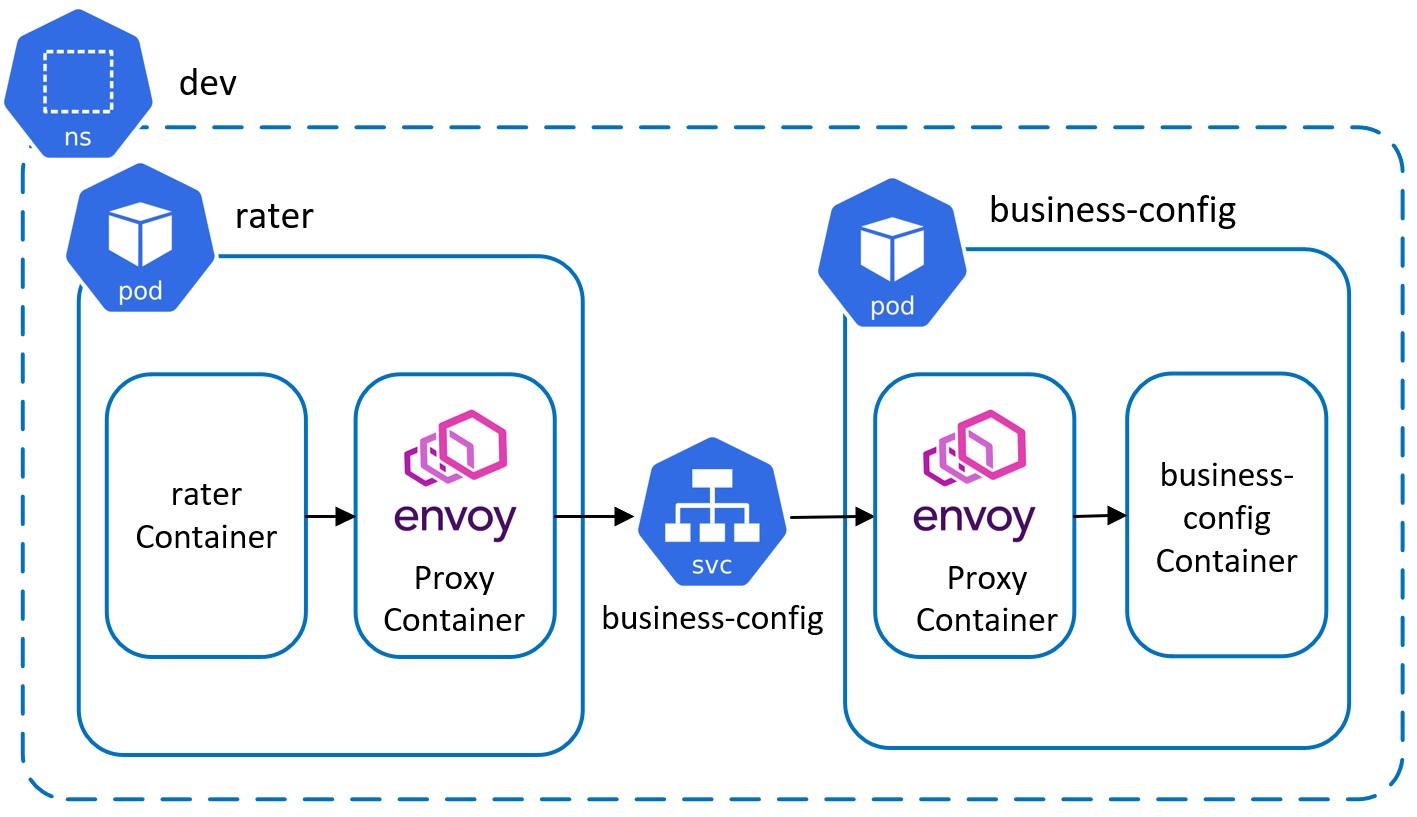
\includegraphics[width=13cm]{img/Sidecar_Pattern.JPG}
		\caption[Istio Sidecar Pattern]{Istio Sidecar Pattern (Eigene Abbildung)}
		\label{sidecar_pattern}
	\end{center}
\end{figure}
\newpage
\section{Bereitstellung ausgewählter Microservices}
\label{Umsetzung_Bereitstellung_Microservices}
Wie bereits in Kapitel \ref{Konzeption_Auswahl_Microservices} konzeptioniert, dienen der Rater- und der Business-Config-Microservice zur prototypischen Portierung von SAP Subscription Billing auf ein Kubernetes Cluster. Für die Portierung des Rater-Microservices wurden zusätzlich eine lokale PostgreSQL-Datenbank sowie der RabbitMQ Message Broker benötigt. Der Business-Config-Microservice hingegen benötigt eine MongoDB-Datenbank und verwendet ebenso RabbitMQ. \\
Die Bereitstellung der zuvor aufgezählten Komponenten wurde erstmalig mit einem Kubernetes \textbf{Deployment} durchgeführt.\\
Ein Kubernetes Deployment basiert generell auf dem \textbf{Replica Set}. Dieses ist ein Controller, der Pods aus einem Pod Template generiert und die Anzahl an bereitgestellten Replikaten eines Pods überwacht. Dabei werden bei Abweichungen Pods terminiert oder zusätzlich gestartet. Grundsätzlich baut ein Deployment auf den Funktionalitäten eines Replica Sets auf und erweitert diese besonders um weitere Funktionalitäten für die Aktualisierung der Anwendung. Dabei kann zum Beispiel ein \textbf{Rollback} der aktualisierten Anwendung durchgeführt werden, welches die Version der Anwendung auf die zuletzt funktionsfähige Version zurückführt und die Pods aktualisiert.\autocite[Vgl.][S. 118, 276]{Luksa.2018}
\\
Für die Bereitstellung der eigentlichen Microservices wurden \textbf{Stateful Sets} verwendet.\\
Ein Stateful Set basiert, wie auch das Deployment, grundsätzlich auf dem Replica Set. In Abgrenzung zu einem Deployment sind die mittels eines Stateful Sets bereitgestellten Pods jedoch statusbehaftet. Dies bedeutet, dass ein Pod eine feste Identität hat, die auch bei einem Neustart wiederhergestellt wird.\autocite[Vgl.][S. 311-312]{Luksa.2018} Die Entscheidung für die Verwendung von Stateful Sets wurde aufgrund der einfacheren Möglichkeiten zum lokalen Testen, Überwachen und Debuggen gewählt, da der Domainname der einzelnen Pods auch bei einer erneuten Bereitstellung eindeutig bleibt.\\
Aus diesen Gründen wurden während der praktischen Umsetzung alle Bereitstellungen, welche zuvor mit einem Deployment umgesetzt wurden, auf Stateful Sets umgestellt, darunter auch die Bereitstellung der Datenbanken und des RabbitMQ Message Brokers.\\
\\
Die clusterinterne Zurverfügungstellung der Pods wurde unter Zuhilfenahme eigenständiger \textbf{Services} realisiert. Ein Service dient als interne Netzwerkschnittstelle für ein logisches Set an Pods. Dadurch können die Service Discovery Funktionalitäten abgedeckt werden, da alle Anfragen an den gleichbleibenden Domainnamen des Service geschickt werden können. Hierfür wurde jeweils pro Pod ein Service erstellt. Eine beispielhafte Implementierung des für den Rater-Microservice erstellten Service ist aus dem Quelltext \ref{quellcode_rater_service} zu entnehmen. \\
Dabei wird bei der Servicedefinition festgelegt, unter welchem Port der Service zur Verfügung steht und an welches Set von Pods die Anfragen weitergeleitet werden sollen. Hierbei erfolgt die Auswahl der Pods über den Labelselektor, der mit den Labels der Pods übereinstimmen muss. Diese Abstraktion hat den Vorteil, dass selbst bei Änderungen am Namen des Pods oder dessen Aktualisierung auf eine neue Version keine Änderungen am Service durchgeführt werden müssen.\\
Jedoch ist zu beachten, dass durch die Verwendung von Stateful Sets ein besonderer Servicetyp für die beiden Microservices benötigt wird. Da diese Pods eine unveränderliche Netzwerkidentität haben, sollten sogenannte \textbf{Headless Services} verwendet werden. Diese entsprechen grundsätzlich den normalen Services und unterscheiden sich lediglich seitens des Nichtvorhandenseins einer clusterinternen \ac{IP}-Adresse. Damit wird im clusterinternen \ac{DNS}-Dienst die direkte \ac{IP}-Adresse der Pods hinterlegt. Demzufolge wird die direkte Kommunikation mit dem Pod selbst ohne Umwege über einen Service ermöglicht. Des Weiteren ist die generelle Verwendung von normalen Services ebenso möglich. Jedoch kann dabei nicht sichergestellt werden, dass bei einer Anwendung, welche mit mehreren Replikaten bereitgestellt ist, immer mit dem gleichen Pod kommuniziert wird.\\
Zusätzlich sollte bei der Verwendung von Headless Services berücksichtigt werden, dass dadurch die Load Balancing Funktionalität der Services umgangen wird.\autocite[Vgl.][]{KubernetesAuthors.20200115}\\
\\
Innerhalb der praktischen Umsetzung wurden keine Headless Services verwendet, da die für den Prototyp verwendeten Komponenten jeweils nur mit einem Replikat bereitgestellt wurden, um den Bedarf an Rechenressourcen zu minimieren.\\
Zudem wurden für die beiden Microserives \textbf{Horizontal Pod Autoscaler} Controller erstellt, welche abhängig von der aktuellen \ac{CPU}-Auslastung der bereitgestellten Podreplikate automatisch zusätzliche Replikate bereitstellen. Hierbei wurde zum Beispiel für den Rater-Microservice festgelegt, dass wenn die \ac{CPU}-Auslastung höher als 85 \% ist, ein weiteres Podreplikat bereitgestellt werden soll.\\
\\
Für die Sicherstellung der Datenpersistenz wurden für die PostgreSQL- und die MongoDB-Instanzen jeweils \textbf{Persistent Volume Claims} definiert. Diese veranlassen die Bereitstellung von \textbf{Persistent Volumes}, welche auf nicht flüchtigem Standardspeicher der \ac{GCP} basieren. Die Typdefinition des Speichermediums wurde mit Hilfe von einer \textbf{Storage Class} umgesetzt. Diese wird direkt mit dem Persistent Volume Claim verknüpft, sodass dieser auf das in der Storage Class definierte Speichermedium zurückgreift. Darüber hinaus wird im Persistent Volume Claim die benötigte Speichergröße des Persistent Volumes definiert. \autocite[Vgl.][S. 196, 198-199]{Luksa.2018}\\
\\
In den Deployment- und Stateful Set-Objekten wurde jeweils die \acsp{URL} der in der Image Registry bereitgestellten Docker-Images angegeben. Zusätzlich wurde ein \textbf{Secret} angelegt, welches die Anmeldeinformationen für die Docker Registry verschlüsselt abspeichert. Dieses Secret wird für die Bereitstellung der Pods verwendet, da für die Verwendung der Docker-Images die Autorisierung gegenüber der SAP eigenen Image Registry benötigt wird.\\
Bei der Bereitstellung der im Deployment definierten Container wird das Docker-Image von der lokalen Container Engine Docker heruntergeladen und anschließend in einem Pod auf dem Kubernetes Cluster bereitgestellt.\\
Die für die beiden Microservices benötigten Docker-Images wurden erstmalig manuell auf dem lokalen Rechner gebaut und in die Image Registry hochgeladen. Jedoch wurde dieser Schritt mit Hilfe der Integration in die \ac{CI}/\ac{CD}-Pipeline vollständig automatisiert. Die Erläuterung der Integration erfolgt in Kapitel \ref{Umsetzung_CI_CD_Integration}. \\
Für die Bereitstellung der RabbitMQ-\footnote{Offizielles RabbitMQ Docker-Image: \url{https://hub.docker.com/_/rabbitmq}}, MongoDB-\footnote{Offizielles MongoDB Docker-Image: \url{https://hub.docker.com/_/mongo}} und PostgreSQL-Pods\footnote{Offizielles PostgreSQL Docker-Image: \url{https://hub.docker.com/_/postgres}} wurde jeweils die aktuellste Version des offiziellen Docker-Images verwendet.\\
Beispielhafte Manifestdateien aller zuvor erwähnten Kubernetes \ac{API}-Objekte und ein beispielhaftes Dockerfile sind im Anhang in Kapitel \ref{quellcode_bereitstellung_microservices} zu finden.


\section{Verschiedene Landschaften}
\label{Umsetzung_Landschaften}
Die erstmalige Umsetzung des Routings der externen Anfragen wurde mittels des Ingress Services von Kubernetes umgesetzt. Eine beispielhafte Manifestdatei für einen Ingress Service ist aus dem Quelltext \ref{quellcode_ingress_service} im Anhang zu finden. Dabei wird innerhalb des Service der extern verfügbare Hostname, wie etwa \url{rater.ingress.k8s-sb.subbilling.shoot.canary.k8s-hana.ondemand.com} und eine Routingregel für die Weiterleitung der an den Hostnamen gesendeten Anfragen definiert. Mit der Routingregel wurde zum Beispiel die Weiterleitung an den erstellten Kubernetes Service des Rater-Microservices festgelegt.\\
\\
Wie in Kapitel \ref{Konzeption_Landschaften} erläutert, wurde das Konzept für das Routing der externen Anfragen durch die Verwendung der folgenden von Istio angebotenen Objekte erweitert:
Virtual Services, Gateways und Destination Rules. 
\\
Ein Istio Virtual Service entspricht grundsätzlich den Services von Kubernetes. Jedoch können mit einem Virtual Service durchaus komplexere Routingregeln definiert werden. 
\newpage
Für die praktische Umsetzung des Anfragenroutings wurden Virtual Services benutzt, da diese unter anderem für das mandantenabhängige Routing der Anfragen, basierend auf den \ac{HTTP}-Headern der Anfrage, verwendet werden können. 
Ein weiterer Vorteil von Virtual Services ist im Vergleich zu den nativen Kubernetes Services zum Beispiel die Möglichkeit eines gewichteten Routings auf unterschiedliche Versionen der bereitgestellten Anwendung.\autocite[Vgl.][S. 153]{Sharma.2020} Damit kann beispielsweise \textbf{Canary Releasing} umgesetzt werden. Dies ist eine Aktualisierungsstrategie, bei der die aktualisierte Anwendung erstmalig an beispielshalber fünf Prozent der Anwender getestet wird, bevor sie für alle Anwender zur Verfügung steht.\autocite[Vgl.][]{Sato.2014}\\ 
\\
Eine Destination Rule wird für das versionsabhängige Routing der Anfragen benötigt. Dabei werden innerhalb der Destination Rule die Subsets der Services definiert, welche sich in ihren Versionen unterscheiden. So ist es durch die Verwendung von Versionslabels möglich, mit ausschließlich einem Service das Routing zu mehreren Versionen einer bereitgestellten Anwendung durchzuführen.
Voraussetzung für das versionsabhängige Routing ist das Vorhandensein der Versionsangabe der Anwendung mittels eines einfachen Kubernetes Labels.\\
Ein Istio Gateway ist vergleichbar mit einem Kubernetes Ingress Service. Dieser dient als Load Balancer mit einer externen Schnittstelle, der die Anfragen an einen Virtual Service weiterleitet. Jedoch unterstützt ein Gateway, im Gegensatz zu einem Ingress Service, keine Routingregeln. Er definiert ausschließlich einen Service, der externe Anfragen an die hinterlegte Hostadresse und die festgelegten Ports zulässt und weiterleitet.\autocite[Vgl.][]{IstioAuthors.2019}\\
Eine Gesamtübersicht, der für das mandantenabhänge Routing der Anfragen implementierten Objekte ist der Abbildung \ref{picture_request_routing} zu entnehmen.
\\
Bei dem dargestellten und praktisch umgesetzten Konzept für das Anfragenrouting wird abhängig vom Mandanten das Routing der Anfrage an den Service in den dafür vorgesehen Kubernetes Namespace durchgeführt. Der Mandant sieht exemplarisch wie folgt aus: \textbf{revcloud-dev-eu10-<teamname>}. Hierfür wurden Routingregeln mittels der Istio Virtual Services definiert, welche abhängig von \ac{HTTP}-Headern die Weiterleitung der Anfrage an den eigentlichen Kubernetes Service durchführen.\\
\\
Wie bereits in Kapitel \ref{Konzeption_Landschaften} erläutert, wurde die Isolation der Landschaften sowie die unerwünschte Kommunikation der Pods aus dem gleichen Namespace mit Network Policies konzeptioniert.
Bei der praktischen Umsetzung wurde jeweils eine Network Policy per Pod in einen Namespace implementiert. Eine beispielhafte Manifestdatei der Network-Policy für den Business-Config-Microservice ist aus dem Quelltext \ref{quellcode_verschiedene_landschaften} zu entnehmen.
\begin{figure}[h]
	\begin{center}
		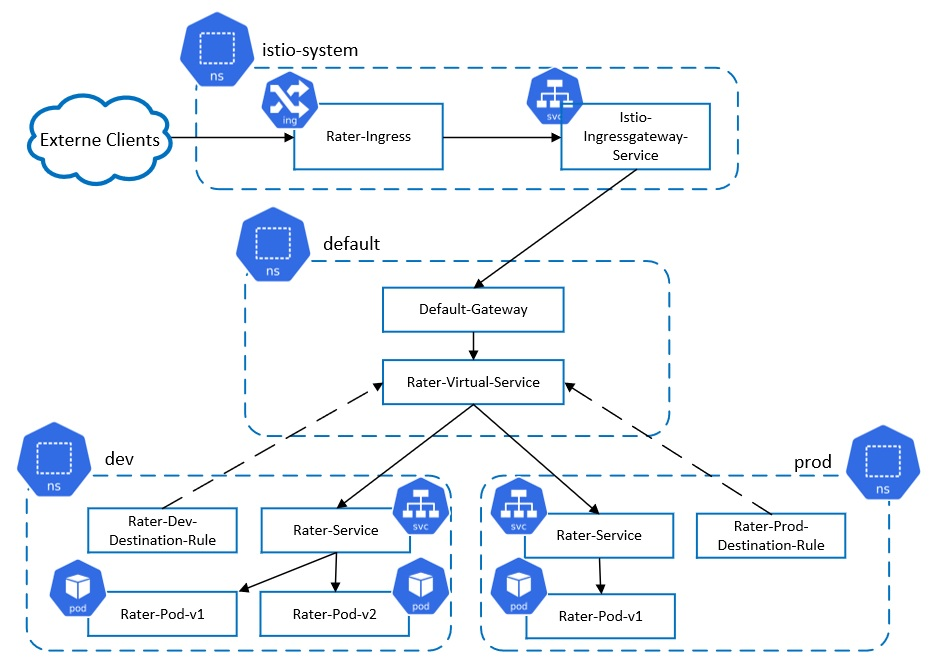
\includegraphics[width=16cm]{img/Landscape_Routing.JPG}
		\caption[Zentrales Routing der Anfragen mit mehreren Landschaften]{Zentrales Routing der Anfragen mit mehreren Landschaften \\(\cite[Eigene Abbildung in Anlehnung an][S. 170]{Sharma.2020})}
		\label{picture_request_routing}
	\end{center}
\end{figure}
\\
Innerhalb der Network Policies wurde die Kommunikation sowohl auf Namespace-Ebene als auch auf Pod-Ebene eingeschränkt. Dabei werden zum Beispiel für den Business-Config-Microservice ausschließlich Anfragen, welche aus dem gleichen Namespace und von Pods, die mit den hinterlegten Labels übereinstimmen, zugelassen.\\
Dadurch konnte die vollständige Unterbindung nicht vorgesehener Kommunikation zwischen den Microservices als auch den Datenbanken umgesetzt werden.
\\
Insgesamt konnte mit Hilfe der Routingobjekte von Istio die Funktionalität für das Routing des aktuell eingesetzten Landscape-Routers vollständig abgedeckt und somit ersetzt werden. Zudem sind weitere Funktionalitäten, wie beispielsweise das zuvor erläuterte Canary Releasing Konzept, möglich.\\
Die beispielhafte Implementierung der zuvor genannten Istio-Objekte für das Anfragenrouting an den Rater-Microservice ist im Anhang unter dem Kapitel \ref{quellcode_verschiedene_landschaften} zu finden.

\section{Integration in die \acs{CI}/\acs{CD}-Pipeline}
\label{Umsetzung_CI_CD_Integration}
Wie in Kapitel \ref{Konzeption_integration_ci_cd_pipeline} konzeptioniert, wurde die Automatisierung der Anwendungsaktualisierung mittels der Integration in die Jenkins \ac{CI}/\ac{CD}-Pipelines umgesetzt.\\
Grundsätzlich existierte zum aktuellen Zeitpunkt der Thesis in dem Subscription Billing Projekt pro Microservice eine eigene Pipeline. Diese wird bei jeder Änderung am hinterlegten Git Repository automatisch ausgeführt. Dabei ist eine Pipeline ein umfangreicher Prozess, welcher die einzelnen \ac{CI}/\ac{CD}-Schritte abarbeitet. Die Deklaration der Pipeline und deren Schritte erfolgt anhand eines \textbf{Jenkinsfiles}.
Eine Pipeline kann, wie in Abbildung \ref{picture_jenkins_pipeline} zu sehen ist, in Stages unterteilt werden, welche zur Gruppierung einzelner Schritte genutzt werden können.\autocite[Vgl.][]{JenkinsAuthors.20190308}\\
Für die Integration der Bereitstellung der Microservices auf das Kubernetes Cluster wurden die Jenkins-Pipelines jeweils um die Stage \textbf{K8s Deployment} erweitert.\\
Die hierfür benötigte Erweiterung des Jenkinsfiles ist im Anhang in Kapitel \ref{quellcode_rater_jenkinsfile} zu finden. Ein Überblick der einzelnen Stages der Pipeline des Rater-Microservice ist der Abbildung \ref{picture_jenkins_pipeline} zu entnehmen. 
\\
\begin{figure}[h]
	\begin{center}
		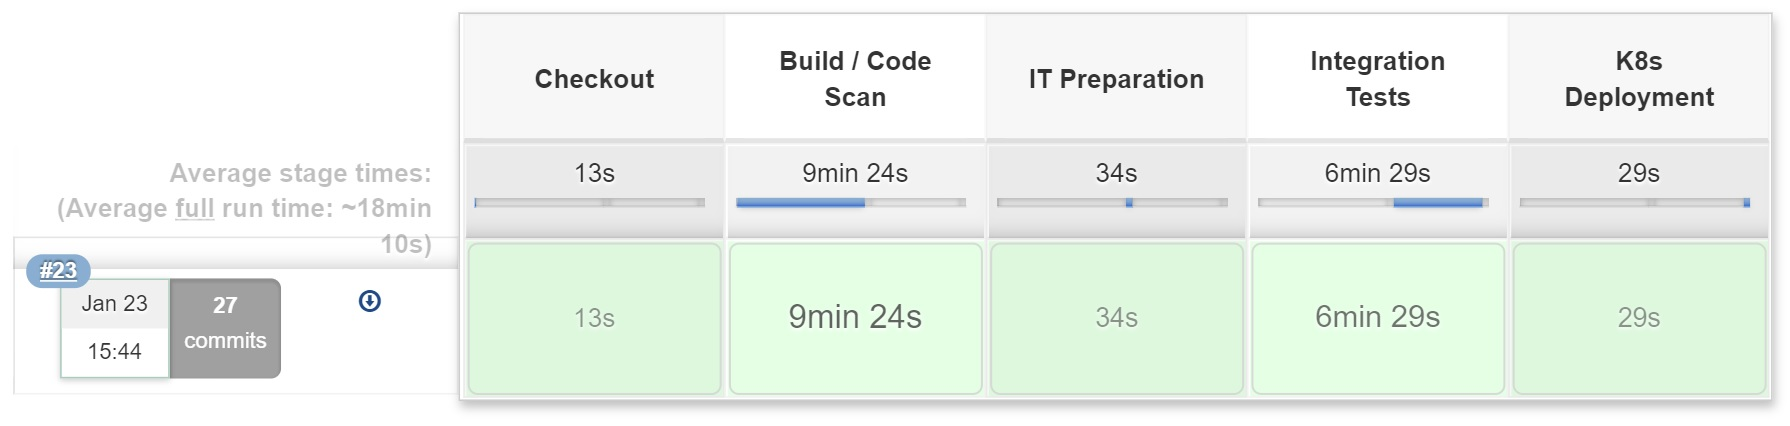
\includegraphics[width=16cm]{img/Jenkins_Pipeline.JPG}
		\caption[Übersicht Stages der Jenkins-Pipeline]{Übersicht Stages der Jenkins-Pipeline\\(Abbildung stammt aus der der Jenkins Pipeline)}
		\label{picture_jenkins_pipeline}
	\end{center}
\end{figure}
\\
Innerhalb der K8s-Deployment-Stage wurden die folgenden Schritte konzeptioniert und implementiert. 
\begin{enumerate}
	\item Bauen des Docker-Images mittels des Artefakts des Microservices, des Dockerfiles und der lokalen Container Engine Docker.
	\item Kennzeichnen des Docker-Images mit dem aktuellen Zeitstempel.
	\item Hochladen des Docker-Images auf die extern verfügbare Image Registry von SAP.
	\item Bereitstellen/Aktualisieren der im Skaffold-Manifest definierten Kubernetes \ac{API}-Objekte auf das Kubernetes Cluster.
\end{enumerate}
Die zuvor genannten Schritte der Stage wurden mit dem Skaffold Tool weiter automatisiert. 
Hierbei ist zu erwähnen, dass der Jenkins-Server selbst auf einem zusätzlichen Kubernetes Cluster bereitgestellt ist.\\ 
In der Pipeline werden jeweils Pods zur Bearbeitung der definierten Stages und deren Jobs generiert. Für die \textbf{K8s Deployment} Stage wurde ein bereits vorhandenes Pod-Template um einen Skaffold Container erweitert. Neben dem Skaffold Tool besitzt der Pod beispielsweise auch einen Container mit der lokalen Container Engine Docker, welche zum Bauen und Hochladen des Docker-Images verwendet wird.\\
Des Weiteren ist zu beachten, dass ohne die Verwendung von Skaffold die Bereitstellung eines Kubernetes-Objektes aus einem Pod eines Clusters in ein anderes Kubernetes Cluster nicht ohne Workarounds möglich gewesen ist.\\
Jedoch konnten die benötigten Workarounds vollständig durch die Verwendung des Skaffold Tools ersetzt werden, da damit der für die Bereitstellung verwendete \textbf{kube-config} festgelegt werden kann. Dieser definiert in welchem Kubernetes Kontext und somit in welchem Kubernetes Cluster die Bereitstellung der definierten Objekte stattfinden soll.\autocite[Vgl.][]{SkaffoldAuthors.20200116}
Dadurch können mit Skaffold auch aus einem Kubernetes Cluster heraus Objekte in einem anderem Kubernetes Cluster bereitgestellt werden. Eine vereinfachte Darstellung des Bereitstellungsprozesses ist in Abbildung \ref{picture_ci_cd_process} zu sehen.\\
Ein weiterer Vorteil von Skaffold ist die Möglichkeit der sogenannten \textbf{skaffold dev}-Funktion. Diese Funktion ermöglicht die Aktualisierung der bereitgestellten Anwendung bei jeder Änderung des Quellcodes. Dies eignet sich besonders in Kombination mit der Verwendung eines Git Repositories. Hierbei kann Skaffold bei jeder Aktualisierung des Git Repositories die automatische Aktualisierung der Anwendung starten.\autocite[Vgl.][]{SkaffoldAuthors.20200116b}\\
Zum aktuellen Zeitpunkt ist die Verwendung dieses Features jedoch nicht geplant, da dies bereits mit der Jenkins-Pipelines umgesetzt wird.
\\
\begin{figure}[h]
	\begin{center}
		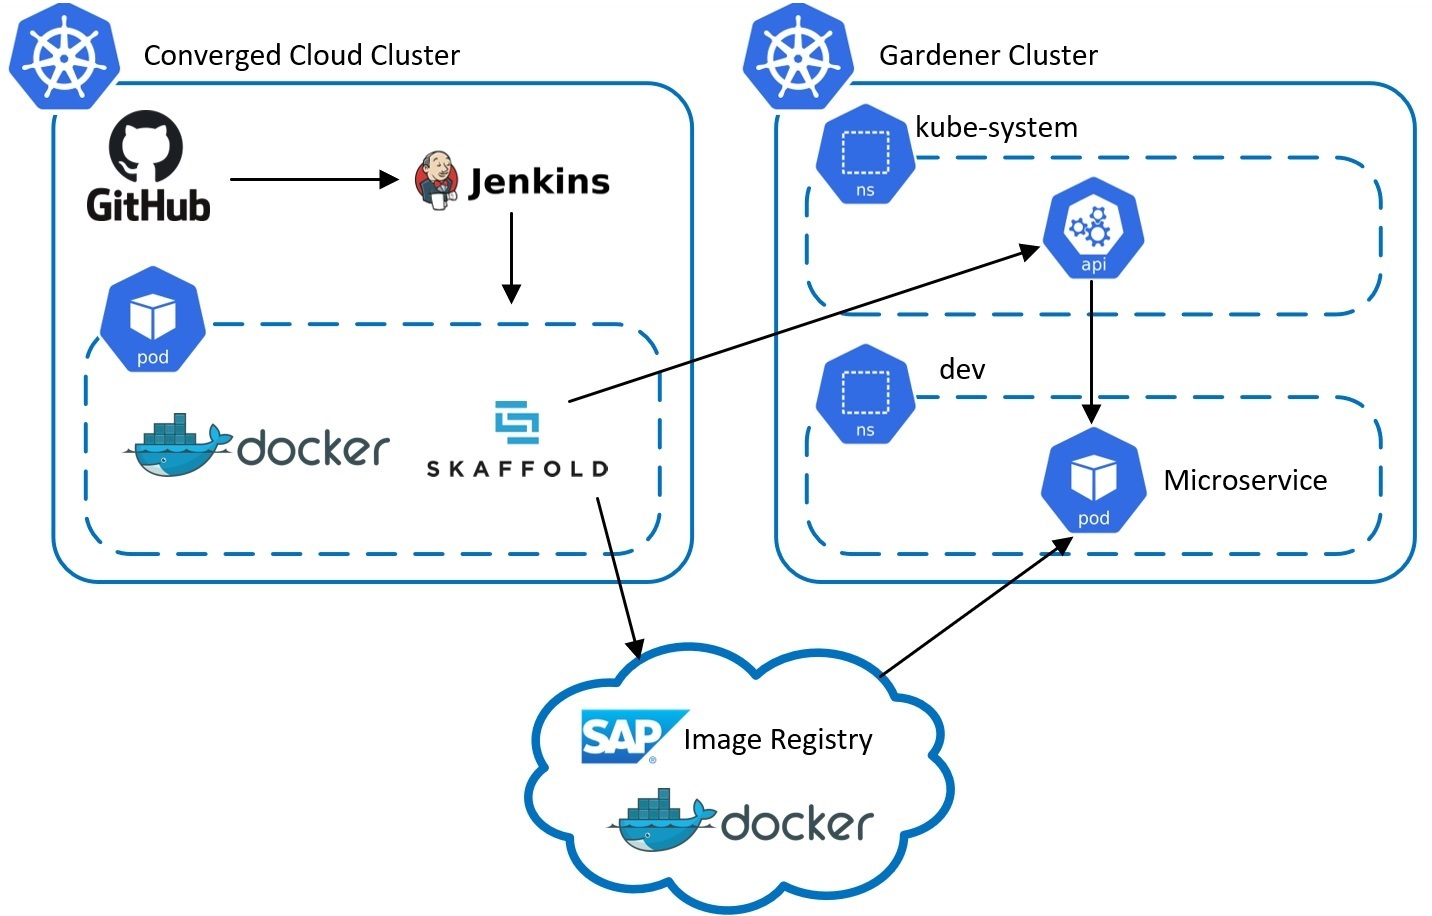
\includegraphics[width=16cm]{img/CI_CD_Integration.JPG}
		\caption[Übersicht Bereitstellungsprozess des Jenkins-Servers]{Übersicht Bereitstellungsprozess des Jenkins-Servers \\
			(Eigene Abbildung)}
		\label{picture_ci_cd_process}
	\end{center}
\end{figure}
\\
Generell ermöglicht Skaffold eine einheitliche Definition der beschriebenen Prozesse mittels einer einzigen Manifestdatei. \\
Eine beispielhafte Manifestdatei für den Rater-Microservice ist im Anhang in Kapitel \ref{quellcode_skaffold_rater} zu finden.\\
Ein zusätzlicher Vorteil von Skaffold ist die Möglichkeit der direkten Angabe des Namespaces bei der Verwendung des \textbf{skaffold run}-Kommandos. Dies kann mit dem \textbf{--namespace}-Tag durchgeführt werden. Dadurch soll bei dem gewählten Multi-Namespace-Konzept der für die Bereitstellung entsprechende Namespace per Tag angegeben werden. Auf diese Weise kann das Erstellen von duplizierten Manifestdateien, welche sich ausschließlich in der Definition des Namespaces unterscheiden, vermieden werden.\\
\newpage
Der Nachteil der Verwendung des Skaffold Tools ist ausschließlich die zusätzliche Manifestdatei für Skaffold und die benötigte Installation der lokalen Skaffold \ac{CLI}. Jedoch konnte dies mit Hilfe der Verwendung der automatischen Bereitstellung durch den Jenkins-Server auf einem zusätzlichen internen Kubernetes Cluster abgelöst werden.\footnote{Weitere Informationen zu Skaffold: \url{https://skaffold.dev/docs/}}\\ 

\section{Service-to-Service Kommunikation}
\label{Umsetzung_S2S_Kommunikation}
Wie bereits in Kapitel \ref{Konzeption_S2S_Kommunikation} erläutert, wurde die erste praktische Umsetzung der Kommunikation der Microservices untereinander mittels der nativen Kubernetes Services umgesetzt. Dabei wurde für jeden Microservice ein eigener Kubernetes Service erstellt, welcher als Schnittstelle für die eingehenden Anfragen anderer Microservices dient. Dabei erfolgt, wie in Kapitel \ref{Konzeption_S2S_Kommunikation} erläutert, die Weiterleitung der Anfragen mit Hilfe des im Service definierten Labelselektors. Eine beispielhafte Manifestdatei für den Service des Rater-Microservices ist aus dem Anhang im Quelltext \ref{quellcode_rater_service} zu finden.\\
\newpage
Da die Kubernetes Services jedoch nativ keine verschlüsselte Service-to-Service Kommunikation unterstützen, wurde das Konzept um die Virtual Services von Istio erweitert. Dabei wurden auch die zuvor implementierten Kubernetes Services benötigt und wiederverwendet.
\\
\begin{figure}[h]
	\begin{center}
		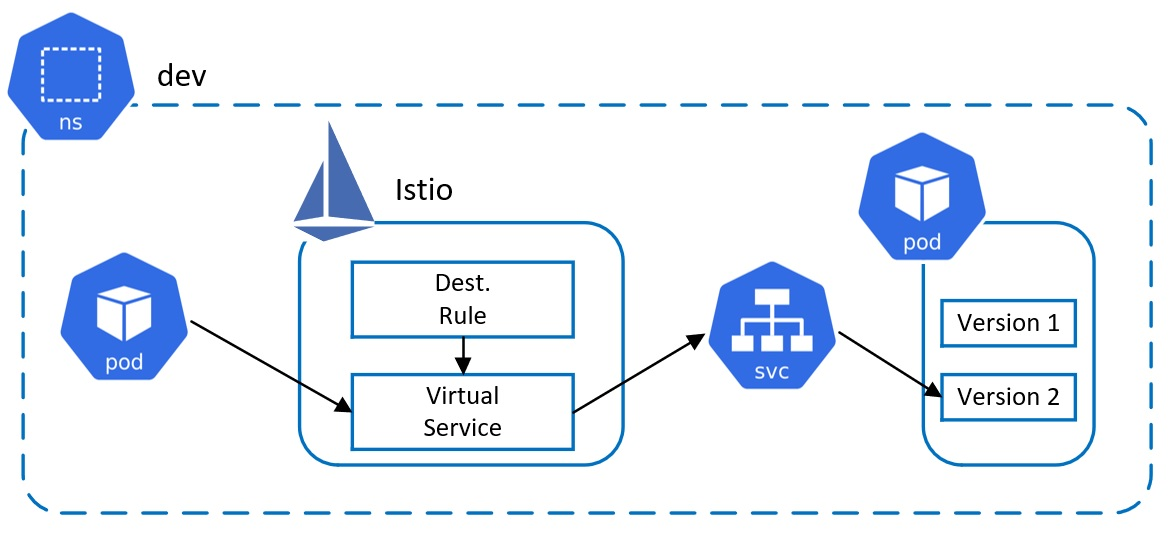
\includegraphics[width=16cm]{img/Istio_S2S_Kommunikation.JPG}
		\caption[Service-to-Service Kommunikation mit Istio]{Service-to-Service Kommunikation mit Istio\\
			(\cite[Eigene Abbildung in Anlehnung an][S. 145]{Sharma.2020})}
		\label{grafik_istio_s2s_kommunikation}
	\end{center}
\end{figure}
\\
Wie der vereinfachten Abbildung \ref{grafik_istio_s2s_kommunikation} zu entnehmen ist, fängt der Virtual Service als erste Komponente die Anfrage ab und leitet diese dann an den hinterlegten Kubernetes Service weiter. Dabei benötigt jeder Virtual Service eine Destination Rule, welche unter anderem die unterschiedlichen Versionen eines Service definiert. Zudem kann auch das für den Lastenausgleich eingesetzte Verfahren, wie beispielsweise das \textbf{Round Robin} Verfahren konfiguriert werden.\autocite[Vgl.][Destination Rule]{IstioAuthors.20191115} Weitere Informationen zu den möglichen Verfahren des Lastenausgleichs sind unter dem angegebenen Link zu finden.\footnote{Verfahren für den Lastenausgleich: \url{https://istio.io/docs/reference/config/networking/destination-rule/\#LoadBalancerSettings-SimpleLB}}\\
Innerhalb der Virtual Services können Routingregeln oder auch \textbf{Failover Szenarien} für auftretende Kommunikationsfehler hinterlegt werden.\\
Bei der praktischen Umsetzung des Prototyps wurde exemplarisch das Failover Szenario für den Virtual Service des Business-Config-Microservices implementiert. Dabei werden zum Beispiel bei einem Kommunikationsfehler mit dem \ac{HTTP}-Statuscode 503, 504 oder 505 jeweils drei erneute Kommunikationsversuche durchgeführt.\\
Eine beispielhafte Manifestdatei für einen Virtual Service ist aus dem Anhang im Quelltext \ref{quellcode_rater_vs} zu entnehmen.\\
\newpage
Generell ist jedoch zu berücksichtigen, dass die vom Service Mesh Istio verwendeten Virtual Services und Destionation Rules sich ausschließlich mittels den in Kapitel \ref{Umsetzung_Bereitstellung_Microservices} erläuterten Envoy Proxies in die interne Netzwerkkommunikation von Kubernetes einklinken können. Hierbei erfolgt die Angabe des Zielservices in einem Microservice weiterhin mit dem nativen Domainnamen des Kubernetes Services und es bedarf keiner Anpassungen an die vom Service Mesh Istio zusätzlich implementierten Objekte. Dies ist beispielsweise im Fall einer Anfrage, welche vom Rater-Microservice an den Business-Config-Microservice gesendet werden soll, die interne \ac{URL}: \url{http://business-config-svc:8080}.\\
\\
Der Hauptgrund für die Verwendung von Virtual Services ist jedoch die Unterstützung von \ac{mTLS}. Dies wurde einerseits mit Hilfe des Konfigurationsmanifests von Istio zentral für alle Services festgelegt. Dadurch wurde das clientseitige \ac{mTLS} aktiviert. Dabei legt die clientseitige Konfiguration von \ac{mTLS} fest, ob die Anfragen an die Services vom Endpunkt des Clients authentifiziert sein müssen.\\
Andererseits wurde die serverseitige Implementierung von \ac{mTLS} durch eine globale \textbf{Policy} umgesetzt. Diese definiert globale Vorschriften für die innerhalb des Clusters stattfindenden Netzwerkkommunikation und ist im Anhang aus dem Quelltext \ref{quellcode_globale_mtls_policy} zu entnehmen. \\
Mit Hilfe der serverseitigen Verwendung von \ac{mTLS} wird die eigentliche Verschlüsselung der Kommunikation umgesetzt.\autocite[Vgl.][Authentication policies]{IstioAuthors.20200106}\\
\\
Mit der Verschlüsselung der clusterinternen Kommunikation konnte bewiesen werden, dass der zentrale Credential Store Vault für die Absicherung der Kommunikation der Microservices nicht mehr benötigt wird. Dies kann dadurch begründet werden, dass bei \ac{mTLS} keine zusätzliche Authentifikation der Microservices mit Hilfe von Credentials eingesetzt werden muss.\\
Des Weiteren konnte die benötigte Service Discovery Funktionalität, die auf der \ac{CF} mit dem zusätzlichen Eureka-Service gelöst wurde, mittels der nativen Kubernetes Services und der Virtual Services von Istio ebenso abgedeckt werden. Dies hat den Vorteil, dass die generelle Verwaltung und der Betrieb des Eureka Services und des Credential Stores Vault bei der Verwendung von Kubernetes nicht mehr benötigt wird.\\
Zudem wurden mit Hilfe der Virtual Services die zuvor beschriebenen Failover Szenarien umgesetzt. Diese sichern beispielsweise eine durch Netzwerkprobleme bedingte, fehlgeschlagene Kommunikation ab.

\section{Monitoring und Logging}
\label{Umsetzung_Monitoring_Logging}
Zur Umsetzung des Loggingkonzeptes wurden, wie in Kapitel \ref{Konzeption_Monitoring_Logging} konzeptioniert, die Komponenten Elasticsearch, Filebeat und Kibana implementiert. Dabei wurde der Helm Package Manger für die Implementierung auf dem Kubernetes Cluster verwendet.\footnote{Verwendeter Installationsguide: \url{https://www.linode.com/docs/applications/containers/how-to-deploy-the-elastic-stack-on-kubernetes/}} 
\\
Hierbei wurde Elasticsearch mittels des Kubernetes-Objektes Stateful Set implementiert. Diese hat im Fall von Elasticsearch den Vorteil, dass die erzeugten Pods einen persistenten Status haben, welcher auch bei einem Neustart des Pods wiederhergestellt wird. Somit gehen im Zusammenspiel mit der Verwendung von Persistent Volume Claims auch bei einem Ausfall eines Elasticsearch Pods keine Daten verloren.\\ 
Filebeat wurde mit einem \textbf{Daemon Set} implementiert, welches grundsätzlich den gleichen Zweck wie ein Deployment verfolgt. Unterschiedlich ist jedoch die Auswahl der für die Bereitstellung des Pods verwendeten Node. Dabei stellt ein Daemon Set sicher, dass mindestens ein Replikat des Pods je Node bereitgestellt wird.\autocite[Vgl.][Daemon Set]{KubernetesAuthors.20191210} Damit eignet es sich optimal für die Bereitstellung von Filebeat, um die Logdateien von allen Nodes in den ELK-Stack extrahieren zu können.\\
Da Kibana ausschließlich als Visualsierungstool verwendet wird, ist hierbei keine Bereitstellung auf jeder Node nötig. Aufgrund dessen wurde es mit einem Deployment auf einer beliebigen Worker Node bereitgestellt.\\
Außerdem wurden für die Komponenten Elasticsearch und Kibana Services erstellt, um deren Dienste innerhalb des Clusters für andere Komponenten zur Verfügung zu stellen. Für Filebeat wurde kein Service benötigt, da diese Komponente des ELK-Stacks ausschließlich die Logdateien an Metricbeat sendet und keine weitere Kommunikation stattfindet. Ein beispielhafter Ausschnitt aus dem Dashboard von Kibana ist im Anhang in Abbildung \ref{anhang_grafik_kibana_dashboard} zu finden.\\
\\
%Monitoring
Für die Umsetzung des Monitoringkonzeptes wurde Dynatrace ebenfalls mit einem Daemon Set implementiert. Dieses sorgt dafür, dass der darin definierte \textbf{One-Agent-Pod} auf allen Nodes bereitgestellt wird. Die One-Agent-Pods extrahieren automatisch die Nutzungsdaten aller auf den Nodes bereitgestellten Pods und senden diese an den festgelegten Dynatrace-Host-Server. Hier sollte beachtet werden, dass für die One-Agent-Pods eine eigenständige System-Rolle angelegt werden muss, welche Berechtigungen auf die Systemdaten hat, um auch auf die Daten der Kubernetes Master Node zugreifen zu können.\\ 
Im direkten Vergleich zur \ac{CF} bietet Kubernetes den Vorteil, dass die One-Agents-Pods hierbei ausschließlich einmal pro Node und nicht, wie bei der \ac{CF}, für jede einzelne Anwendung bereitgestellt werden müssen.\\
Generell ermöglicht Dynatrace die Überwachung auf allen vorhandenen Ebenen, wie beispielsweise auf gesamter Node-Ebene, als auch auf granularer Prozess-Ebene der einzelnen Container, welche in einem Pod auf einer der Nodes bereitgestellt sind.\footnote{Verwendeter Guide: \url{https://www.dynatrace.com/support/help/technology-support/cloud-platforms/kubernetes/installation-and-operation/full-stack/deploy-oneagent-on-kubernetes/}}\\
Eine beispielhafte Übersicht aus dem Dynatrace Dashboard für das Monitoring der Auslastung einer Worker Node ist im Anhang in der Grafik \ref{anhang_grafik_dynatrace_dashboard} zu finden.\\
\\
Generell sollte bei der praktischen Umsetzung der Konzepte für das Monitoring und Logging des Kubernetes Clusters beachtet werden, dass die implementierten Komponenten ausschließlich innerhalb des Clusternetzwerkes verfügbar sind und aus Sicherheitsgründen keine extern erreichbare Zugangspunkte angelegt wurden.\\ 
Jedoch wird dies für die Evaluation des Prototyps nicht benötigt, da hierfür ein temporärer Zugangspunkt für den lokalen Rechner mittels des \textbf{port-forward}-Kommandos der Kubernetes \ac{CLI} manuell erstellt werden kann. Dabei werden die Anfragen an den \textbf{localhost} automatisch an den Service des Kubernetes Clusters weitergeleitet und somit ein temporärer Zugriff auf die clusterinternen Services ermöglicht.\footnote{Guide für lokaler Zugriff auf clusterinterne Services: \url{https://kubernetes.io/docs/tasks/access-application-cluster/port-forward-access-application-cluster/}} 

% !TEX root =  master.tex
\chapter{Evaluation des Kubernetes Prototyps}
\label{Evaluation_K8s}
In den folgenden Unterkapiteln erfolgt das Testen der Funktionsweise des auf dem Kubernetes Cluster bereitgestellten Prototypen. Zudem werden mit Hilfe der bei der Umsetzung des Prototyps gesammelten Erfahrungen und den Ergebnissen der theoretischen Untersuchung der Prototyp und Kubernetes selbst evaluiert.
\section{Testen des Kubernetes Prototyps mittels API-Calls}
Um die vollständige Funktionalität der bereitgestellten Microservices zu testen, wurden die bereits vorhandenen Integrationstests der Microservices durchgeführt. Diese wurden mittels des internen Test-Frameworks gegen die \ac{API}-Endpunkte der Microservices ausgeführt. Dabei wurde unter anderem auch die Service-to-Service Kommunikation getestet, da der Rater-Microservice für einige der ausgeführten Integrationstests vom Business-Config-Microservice abhängig ist.\\
Insgesamt wurden alle Integrationstest erfolgreich ausgeführt, sodass die Funktionalität des bereitgestellten Prototyps auf dem Kubernetes Cluster bestätigt werden kann.
\section{Bewertung der prototypischen Infrastrukturlösung}
\label{bewertung_k8s_prototyp}
Die Evaluation der prototypischen Bereitstellung der SAP Subscription Billing Lösung in einem Kubernetes Cluster erfolgt, wie auch die Evaluation der aktuellen Infrastrukturlösung, mit Hilfe der in Kapitel \ref{kapitel_merkmale_vorgehensweise} definierten Vergleichsmerkmale und Vorgehensweise.
\begin{description}
\item[Performance] \hfill \\
	Bei der Messung der Performance des Kubernetes Clusters wurde die gleiche \ac{HTTP}-Anfrage, welche auch zur Evaluation der \ac{CF}-Plattform eingesetzt wurde, verwendet. Das gesamte Testsetup ist im Anhang in Kapitel \ref{anhang_performancetests} zu finden. Bei der Evaluation des Kubernetes Prototypen wurden, die in der Tabelle \ref{tabelle_performance_k8s} dargestellten Durchschnittswerte ermittelt.
	\begin{table}[ht]
		\centering
		\begin{tabular}[h]{c|c|c|c}
			Threads & Anzahl Anfragen & Antwortzeit pro Anfrage & Durchsatz pro Sekunde \\
			\hline
			100 & 330717,4 & 88,6 ms & 1095,60 
			\\
			\hline
			150 & 305489,4 & 144,4 ms & 1145,85
			\\
			\hline
			200 & 312006,2 & 188,8 ms & 1020,78
			\\
		\end{tabular}\\
	\caption{Ergebnisse Performancetets: Kubernetes Cluster in Belgien}
	\label{tabelle_performance_k8s}
	\end{table}
	\\
	Eine erweiterte Darstellung aller einzelnen Testläufe mit zusätzlichen Variablen ist im Anhang in Kapitel \ref{section_performance_k8s_gardener} und \ref{section_performance_k8s_con_cloud} zu finden.\\
	Da die dabei ermittelten Durchschnittswerte unerwartet schlechter als die in Kapitel \ref{bewertung_cf} dargestellten Ergebnisse der \ac{CF} gewesen sind, wurden zusätzliche Performancetests auf einem weiteren Kubernetes Cluster durchgeführt. Dabei wurde der Rater-Microservice auf dem abteilungsinternen Kubernetes Cluster, das bereits in Kapitel \ref{Konzeption_integration_ci_cd_pipeline} erwähnt wurde, bereitgestellt. Dabei wurden folgende Durchschnittswerte ermittelt.
	\begin{table}[ht]
		\centering
		\begin{tabular}[h]{c|c|c|c}
			Threads & Anzahl Anfragen & Antwortzeit pro Anfrage & Durchsatz pro Sekunde \\
			\hline
			100 & 387270,4 & 75,6 ms & 1290,33 
			\\
			\hline
			150 & 371185,4 & 118,6 ms & 1234,62
			\\
			\hline
			200 & 339434,6 & 173,6 ms & 1127,37
			\\
		\end{tabular}\\
		\caption{Ergebnisse Performancetets: Kubernetes Cluster in Frankfurt}
	\end{table}
	\\
	Die dabei ermittelten Testergebnisse bestätigten die Vermutung, dass die unterschiedliche Performance zwischen der \ac{CF} und dem mittels Gardener provisionierten Kubernetes Cluster hauptsächlich durch die Latenzunterschiede begründet werden können.	Der Latenzunterschied erklärt sich anhand der Verwendung der unterschiedlichen Infrastrukturen. Dabei basiert die \ac{CF} auf der \ac{AWS}-Infrastruktur in einem Rechenzentrum in Frankfurt, wohingegen das für den Prototyp verwendete Kubernetes Cluster aus Kostengründen in einem der \ac{GCP}-Rechenzentren in Belgien betrieben wird.
	\\
	\begin{figure}[h]
		\begin{center}
			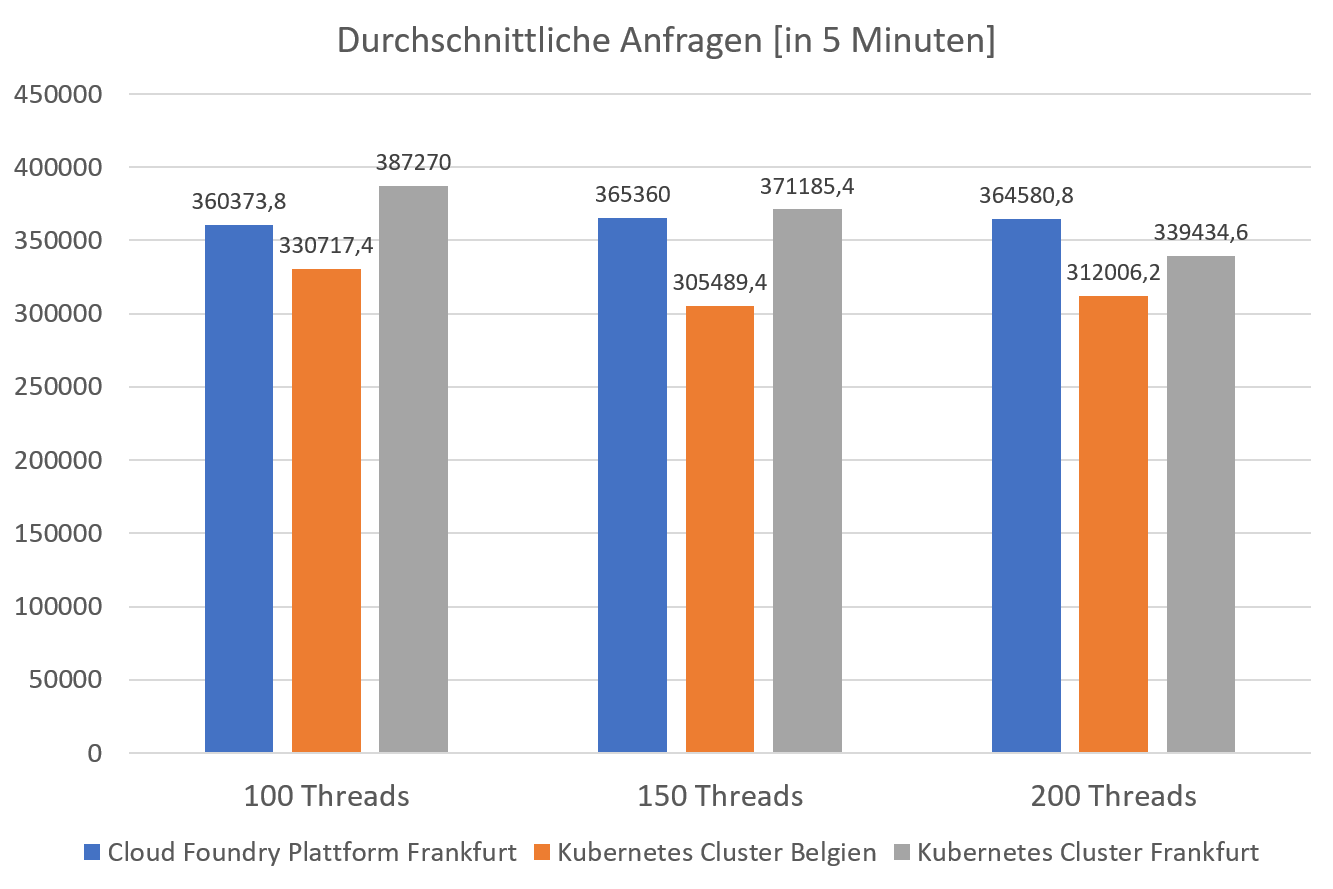
\includegraphics[width=13cm]{img/Performance_Response_Amount.PNG}
			\caption[Ergebnisse Performancetests: Anzahl beantworteter Anfragen]{Ergebnisse Performancetests: Anzahl beantworteter Anfragen}
			\label{performance_anzahl_antworten}
		\end{center}
	\end{figure}
	\begin{figure}[h]
		\begin{center}
			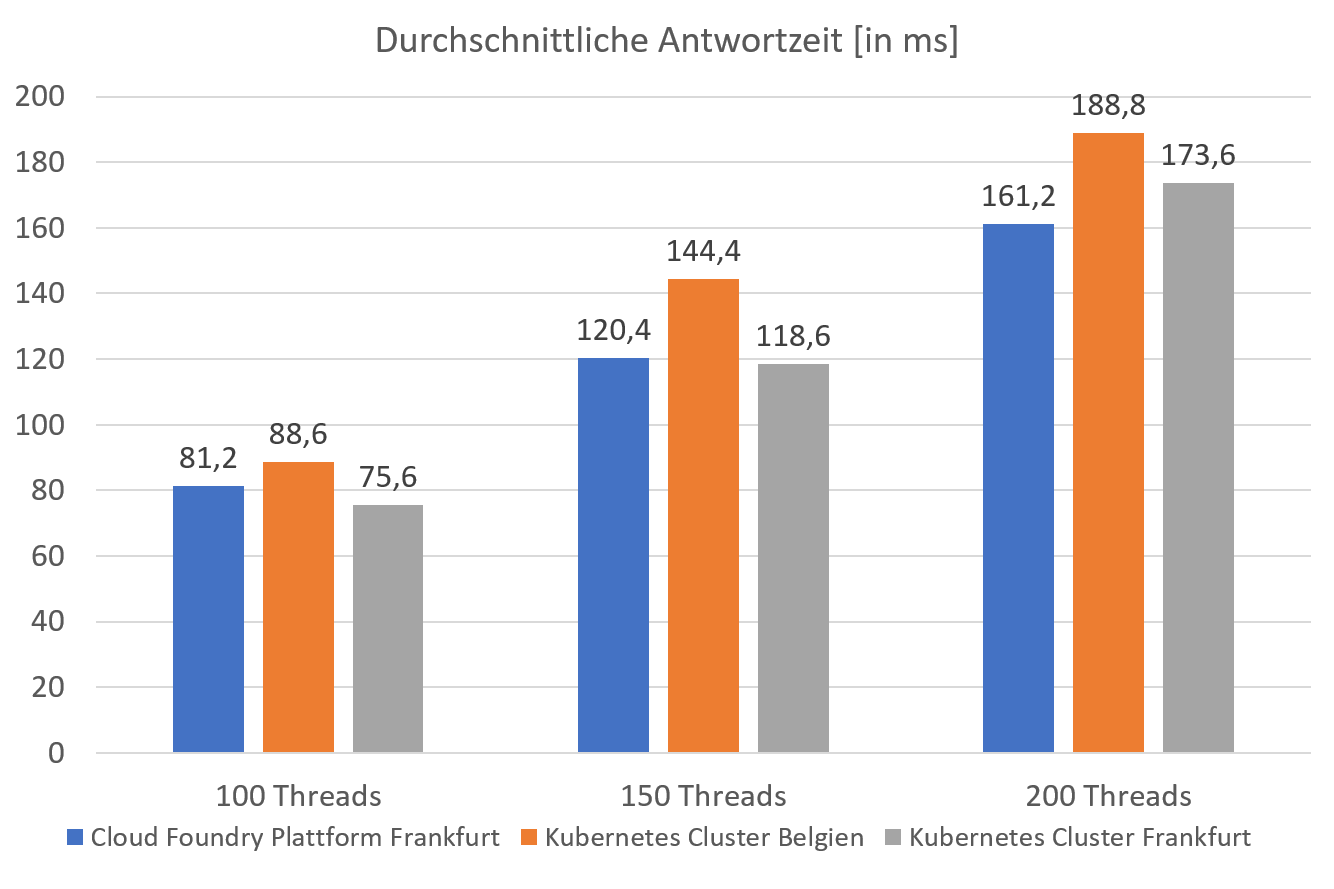
\includegraphics[width=13cm]{img/Performance_Response_Time.PNG}
			\caption[Ergebnisse Performancetests: Durchschnittliche Antwortzeit der Anfragen]{Ergebnisse Performancetests: Durchschnittliche Antwortzeit der Anfragen}
			\label{performance_antwortzeit}
		\end{center}
	\end{figure}
	\\
	%Anmerkung: Siehe Abstand Formattierung
	Das zusätzlich verwendete Cluster wurde ausgewählt, da es ebenfalls in Frankfurt betrieben wird und somit eine bessere Vergleichbarkeit mit der \ac{CF} besteht.\\
	Wie den Abbildungen \ref{performance_anzahl_antworten} und \ref{performance_antwortzeit} zur Gegenüberstellung der Ergebnisse der Performancetests der unterschiedlichen Plattformen und Kubernetes Clustern zu entnehmen ist, gibt es grundsätzlich keine bemerkenswerte Performanceunterschiede zwischen der \ac{CF} und Kubernetes. Dabei konnte \ac{CF} besonders bei einer höheren Anzahl an parallelisierten Anfragen besser als das Kubernetes Cluster abschneiden. Wohingegen der auf dem Kubernetes Cluster bereitgestellte Rater-Microservice bei einer geringeren Anzahl an parallelisierten Anfragen eine geringere durchschnittliche Antwortzeit pro Anfrage und somit eine bessere Performance als der auf der \ac{CF} bereitgestellte Rater-Microservice aufzeigte.\\
\item[Kosten] \hfill \\
	Da Kubernetes und das Gardener Projekt Teil der Open Source Community sind, fallen hierfür keine generellen Servicekosten an. Die für den Betrieb des Kubernetes Clusters anfallenden Kosten setzen sich somit ausschließlich aus den Kosten des \ac{IaaS}-Providers zusammen. Dies sind bei der Verwendung des \ac{GCP} Kosten für die \acsp{VM}, für die persistenten Datenspeicher sowie für die benötigten Load Balancer.\\
	Jedoch werden im Rahmen des Kostenvergleiches der vorliegenden Thesis aus Gründen der Vergleichbarkeit explizit die Kosten für die Application Runtime verwendet.\\
	Dabei können bei der \ac{GCP} folgende sich an die Vergleichswerte von 34 und 780 \ac{GB} \ac{RAM} annähernden Konstellationen eingesetzt werden.\\
	$\textrm{Monatliche Kosten 33,75 \ac{GB} \ac{RAM}:}\\
	= 1 \textrm{x n1-standard-8} + 1 \textrm{x n1-standard-1} \\
	= 30 \textrm{ \ac{GB} \ac{RAM}} + 3,75 \textrm{ \ac{GB} \ac{RAM}}\\
	= 227,27\textrm{\euro} + 28,40\textrm{\euro} = 255,67\textrm{\euro}\\
	\\
	\textrm{Monatliche Kosten 780 \ac{GB} \ac{RAM}:}\\
	= 2 \textrm{x n1-standard-96} + 1 \textrm{x n1-standard-16} \\
	= 720 \textrm{ \ac{GB} \ac{RAM}} + 60 \textrm{ \ac{GB} \ac{RAM}}\\
	= 5458,73\textrm{\euro} + 454,89\textrm{\euro} = 5913,62\textrm{\euro}\\$	
	\\
	Die für die Berechnung verwendeten Kostenangaben stammen von der offiziellen Kostenübersicht der \ac{GCP}.\footnote{Zur Kostenberechnung der \ac{GCP}: \url{https://cloud.google.com/products/calculator/\#&id=f50cd85a-403a-42de-b5dd-fce73f42ecd0}} Da das Angebot der \ac{GCP} nicht mit dem genauen Angebot der \ac{SCP} übereinstimmt, wurden die annähernden Vergleichswerte von 33,75 \ac{GB} \ac{RAM} und 780 \ac{GB} \ac{RAM} gewählt.
	Jedoch ist hierbei zu beachten, dass es sich, anders als bei der \ac{CF}-Umgebung der \ac{SCP}, nicht um feste monatliche Kosten, sondern um ein Pay-Per-Usage-Kostenmodell handelt.\\ 
	Wie bereits in Kapitel \ref{theorie_saas} beschrieben, hat dieses Kostenmodell den großen Vorteil, dass man als Benutzer der Dienste der \ac{GCP} ausschließlich für den tatsächlichen Verbrauch an Rechenressourcen zahlen muss.\\
	Zusätzlich fallen für das Logging des umgesetzten Prototyps keine generellen Servicekosten an, wie es bei der \ac{SCP} der Fall ist. Allerdings muss hierbei beachtet werden, dass der eigens bereitgestellte ELK Stack Rechenressourcen des Clusters konsumiert.\\
\item[Sicherheit] \hfill \\
Im Bereich der Sicherheit zeichnet sich Kubernetes besonders durch das standardmäßige Nichtvorhandensein von extern verfügbaren Endpunkten aus. 
Die auf dem Kubernetes Cluster bereitgestellten Anwendungen und Services sind, wenn nicht explizit gewünscht, ausschließlich im internen Netzwerk des Clusters verfügbar und es existiert keine extern verfügbare \ac{IP}-Adresse.\\
Ein weiterer Sicherheitsaspekt konnte durch die clusterweite Verwendung von \ac{mTLS} erreicht werden. Damit ist die gesamte Kommunikation sowie die Übertragung von Daten abgesichert und verschlüsselt. Zudem ist eine Kommunikation der Microservices ausschließlich nach der erfolgreichen Authentifikation möglich.\autocite[Vgl.][]{IstioAuthors.20200106} \\
\newpage
Die für die \ac{mTLS}-Verschlüsselung benötigten Zertifikate und Tokens werden automatisch bei der Bereitstellung einer Anwendung in einem Istio aktivierten Namespace generiert. Diese werden unter Zuhilfenahme von Kubernetes Secrets im entsprechenden Namespace abgelegt.\\
Des Weiteren wurde, wie in Kapitel \ref{Umsetzung_Landschaften} beschrieben, mit Hilfe von Network Policies die nicht vorgesehene Kommunikation zwischen Microservices komplett unterbunden. Dadurch können ausschließlich die explizit in den Network Policies definierten Microservices miteinander kommunizieren. Auch die Isolation der Namespaces konnte mit den Network Policies erfolgreich umgesetzt werden, sodass keine ungewollte Kommunikation zwischen Microservices aus unterschiedlichen Namespaces stattfinden kann. Zusätzlich wurden die Zugriffe auf die jeweiligen Datenbanken ausschließlich für die vorgesehenen Microservices eingeschränkt. Damit konnte die zusätzliche Absicherung der Datenbanken erfolgreich umgesetzt werden.\\
Die clusterinternen Konfigurationen, wie beispielsweise die Zugangsdaten für die Image Registry, wurden mit Secrets verschlüsselt im Cluster hinterlegt und somit auch abgesichert.\\
Der Kubernetes \ac{API}-Server wird durch die folgende Sicherheitsvorkehrungen geschützt. Der Zugriff kann zum einen von der \textbf{kubectl} \ac{CLI}, von Kubernetes-Objekten selbst oder auch von externen \ac{REST}-Anfragen erfolgen. Dabei wird die Authentifikation und Autorisierung mittels \textbf{User Accounts} und \textbf{Service Accounts} durchgeführt. User Accounts werden für die Benutzer des Kubernetes Clusters verwendet. Hierbei sollte beachtet werden, dass diese innerhalb des Clusters global gültig sind, weshalb hierfür eine eindeutige Bezeichnung gewählt werden sollte. Service Accounts werden hingegen für die Authentifikation und Autorisierung der eigentlichen Prozesse der Pods eingesetzt. Diese sind hingegen spezifisch einem Namespace zugeordnet.\autocite[Vgl.][]{KubernetesAuthors.20190506}
\\
Der externe Zugriff eines Benutzers wird durch die Verwendung der \ac{CLI} mit Hilfe des benötigten Root-Zertifikates authentifiziert. Dieses ist normalerweise in der lokalen Kubernetes Konfigurationsdatei gespeichert. Im Fall der Provisionierung des Clusters mit Gardener kann dieses direkt aus dem eigenen Gardener Dashboard heruntergeladen werden.\autocite[Vgl.][]{KubernetesAuthors.20191106}\\
Innerhalb des Clusters sind die Sicherheitsmechanismen des \ac{API}-Servers durch die \ac{RBAC} umgesetzt. Dabei werden interne Rollen angelegt, welche unterschiedliche Berechtigungen haben. Eine solche kann beispielsweise eine Berechtigung mit einem ausschließlich lesenden Zugriff auf die in einem Namespace vorhandenen Secrets sein. Die Rollen werden mit \textbf{Role Bindings} an die Benutzer des Clusters gebunden.\autocite[Vgl.][]{KubernetesAuthors.20191023}\\
Somit können mit der \ac{RBAC} umfangreiche Berechtigungskonzepte umgesetzt werden. Jedoch ist zu erwähnen, dass im Rahmen der prototypischen Portierung kein Berechtigungskonzept umgesetzt worden ist, da ausschließlich der Autor der vorliegenden Thesis Zugriff auf das Kubernetes Cluster hatte.\\
\item[Verfügbarkeit] \hfill \\
Grundsätzlich ist die Verfügbarkeit des Kubernetes Clusters ausschließlich von der Verfügbarkeit der Infrastruktur abhängig. Im Fall des umgesetzten Prototyps gibt die \ac{GCP} laut \ac{SLA} aktuell eine Verfügbarkeit der virtuellen Maschinen von mindestens 99,99\% pro Monat an.\autocite[Vgl.][]{GoogleCloudAuthors.20200113}\\
\\
Für die Sicherstellung der clusterinternen Verfügbarkeit der bereitgestellten Anwendungen bietet Kubernetes folgende Mechanismen und \ac{API}-Objekte an.\\ 
Durch die Verwendung von \textbf{Liveness Probes}, \textbf{Startup Probes} und \textbf{Readiness Probes} kann jeweils das generelle Vorhandensein der Anwendungsbereitstellung, das erfolgreiche Starten als auch die Funktionalität der Anwendung überprüft werden. Hierbei können die Proben als \ac{HTTP}- oder \ac{TCP}-Anfragen umgesetzt werden. Eine weitere Möglichkeit zur Überprüfung des Status ist das Ausführen von Kommandos innerhalb des bereitgestellten Containers.\\
Im Vergleich zu \ac{CF} sind die umfangreichen Konfigurationsmöglichkeiten der von Kubernetes angebotenen Proben durchaus hervorzuheben. Mit der Konfigurationseinstellung \textbf{initialDelaySeconds} kann beispielsweise eine initiale Verzögerung für die Überprüfung des Anwendungsstatus, mit den \textbf{timeoutSeconds} die genaue Timeoutzeit der Proben oder mit \textbf{failureThreshold} die maximale Anzahl an Neustarts des Pods konfiguriert werden.\autocite[Vgl.][]{KubernetesAuthors.20200112}\\
\\
Zudem unterstützt Kubernetes das \textbf{Multi Zonen Konzept}, welches zur weiteren Steigerung der Verfügbarkeit dient. Dabei kann ein Cluster in mehreren \textbf{Failure Zones} eines \ac{IaaS}-Providers bereitgestellt werden. Dies bedeutet, dass innerhalb eines Clusters Worker Nodes verwendet werden können, die auf \acsp{VM} aus unterschiedlichen Zonen basieren.\\ 
Der große Vorteil dabei ist, dass bei einem Ausfall einer Zone eines \ac{IaaS}-Providers nicht alle Worker Nodes auf einmal ausfallen. Generell kann dadurch besonders die generelle Resilienz der \ac{SaaS}-Lösung verbessert werden.\\
\newpage
Allerdings sollte bei der Umsetzung des Multi Zonen Konzeptes beachtet werden, dass aus Latenzgründen der Netzwerkkommunikation keine zu sehr voneinander entfernten Zonen in einem Cluster verwendet werden sollten.\autocite[Vgl][]{KubernetesAuthors.20190612}\\
\\
Ein weiteres auf dem Multi Zonen Konzept aufbauendes Projekt ist das \textbf{Cluster Federation Projekt}. Dabei wird das Multi Zonen Konzept um das Ziel der Verwendung mehrerer \ac{IaaS}-Provider erweitert. Vor allem auch On-Premise Cluster sollen dabei unterstützt werden. Dies wird durch die virtuelle Aggregation mehrerer Cluster zu einem einzigen umgesetzt. Das Hauptziel des Cluster Federation Konzeptes ist die Maximierung der Verfügbarkeit. Dies soll beispielsweise durch die Auslagerung von Rechenlast auf ein in der Public-Cloud gehostetes Cluster ermöglichen, falls die Rechenkapazitäten des On-Premise Clusters nicht mehr ausreichen sollten.\autocite[Vgl][]{KubernetesCommunity.20150820}\\
Dennoch muss beachtet werden, dass es sich hierbei um ein Projekt handelt, das in der Version \textbf{v1} veraltet\autocite[Vgl][]{KubernetesAuthors.20191021} und in der Version \textbf{v2} aktuell noch in der Alpha Phase ist.\autocite[Vgl][]{GitHubRepositoryKubernetesSIG.20190815}\\
\item[Skalierbarkeit] \hfill \\
Generell ermöglicht Kubernetes die Skalierbarkeit auf unterschiedlichen Ebenen. Dabei unterstützen zum Beispiel mittels Gardener oder der \ac{GKE} provisionierte Cluster unter anderem die Skalierung auf der gesamten Node-Ebene. Dies bedeutet, dass abhängig von der aktuellen Auslastung der Worker Nodes zusätzliche \acsp{VM}, welche als weitere Worker Nodes dienen, dynamisch bereitgestellt werden können.\autocite[Vgl][]{GitHubRepositoryGardener.20190401}\\
%\footnote{Gardener Node Autoscaler: \url{https://github.com/gardener/autoscaler}}
Bei Gardener kann für die automatische Skalierung auf Worker Node Ebene beispielsweise eine Zielauslastung der \ac{VM}-Instanzen und der Instanztyp angegeben werden. Dabei wird bei einer Überschreitung der Zielauslastung automatisch eine weitere \ac{VM}-Instanz von dem \ac{IaaS}-Provider provisioniert.\autocite[Vgl][]{KubernetesAuthors.20191126}\\
\\
Des Weiteren kann mit Hilfe des \textbf{Horizontal Pod Autoscalers}, welcher auch im Prototyp implementiert worden ist, eine automatische, horizontale Skalierung auf Pod-Ebene umgesetzt werden. Dabei wird vergleichbar mit der Skalierung auf Node-Ebene, bei der Überschreitung der Zielauslastung des Pods ein weiteres Podreplikat generiert.\\
\\
Zusätzlich kann durch das \textbf{Vertical Pod Autoscalers} Projekt auch eine automatische vertikale Skalierung der Pods umgesetzt werden. Dies bedeutet, dass die für die Container der Pods zur Verfügung stehenden Rechenressourcen dynamisch skaliert werden können. Jedoch handelt es sich zum aktuellen Zeitpunkt der Thesis hierbei noch um eine Funktionalität, die sich aktuell noch im Alpha Status befindet und mit einer Custom Ressource Definition implementiert werden muss, weshalb diese innerhalb des Prototyps nicht umgesetzt wurde.\autocite[Vgl][]{GitHubRepositoryKubernetes.20191127}%\footnote{Kubernetes Vertical Pod Autoscaler: \url{https://github.com/kubernetes/autoscaler/tree/master/vertical-pod-autoscaler}}
\\
\item[Konfigurierbarkeit] \hfill \\
Die Erkenntnisse aus der praktischen Umsetzung des Kubernetes Prototyps haben gezeigt, dass Kubernetes im Punkt der Konfigurierbarkeit generell keine Einschränkungen vorsieht.\\
Dabei können alle Objekte des Kubernetes \ac{API}-Servers manuell mit der jeweiligen Manifestdatei oder der \ac{CLI} konfiguriert werden. Besonders die umfangreiche Konfigurierbarkeit der Proben zur Überprüfung der Verfügbarkeit der bereitgestellten Anwendungen erwies sich als hilfreich und konnte einige Probleme lösen, welche bisher innerhalb der aktuellen Infrastrukturlösung aufgetreten sind.\\ Ein Beispiel dafür ist das fehlerhafte Terminieren einer Anwendung bei einer kurzzeitig erhöhten Antwortzeit, obwohl diese eigentlich funktionsfähig gewesen ist. Dieses beispielhafte Problem konnte durch die Erhöhung der Timeoutzeiten bei der Umsetzung des Kubernetes Prototyps gelöst werden.\\
Generell bietet Kubernetes mit den Custom Ressource Definitions die zusätzliche Möglichkeit an, eigene Kubernetes \ac{API}-Objekte zu erstellen und innerhalb des Clusters zu verwenden. Allerdings war dies in der vorliegenden Arbeit nicht notwendig, da alle benötigten Funktionalitäten durch Kubernetes native oder von Istio implementierter \ac{API}-Objekte abgedeckt wurden.\autocite[Vgl.][]{KubernetesAuthors.20191210}\\
\item[Erweiterbarkeit] \hfill \\
Bezüglich der Erweiterbarkeit der bereitgestellten Anwendungen sehen die hierfür benutzten Kubernetes-Objekte mehrere Aktualisierungsstrategien vor.\\
Die für den Prototyp verwendete \textbf{Rolling Update} Strategie ähnelt sehr stark der Blue-Green Deployment Strategie der \ac{CF}. Jedoch unterscheiden sich diese bei der Aktualisierung einer Anwendung, welche mit mehreren Replikationen bereitgestellt ist. Dabei wird in der Rolling Update Strategie jeweils schrittweise die festgelegte Anzahl an Replikation zusätzlich bereitgestellt. 
\newpage
Wenn diese Bereitstellung erfolgreich gewesen ist, wird die gleiche Anzahl an replizierten Pods, welche nicht mehr aktuell sind, terminiert. \\
Dieser Vorgang wird so lange wiederholt, bis alle replizierten Pods schrittweise aktualisiert sind.\\
Generell bietet dies den Vorteil, dass während der Aktualisierung der Anwendung mit mehreren replizierten Pods nicht gleichzeitig alle Podreplikate zusätzlich in der aktualisierten Version bereitgestellt werden müssen. Durch die Verwendung der Rolling Update Strategie können die für die Aktualisierung der Anwendung zusätzlich benötigten Rechenressourcen insgesamt minimiert werden.\\
Zudem kann bei der Verwendung eines Kubernetes Deployments der genaue Prozentsatz an gleichzeitig aktualisierten Pods sowie der hierfür benötigte maximale Ressourcenbedarf konfiguriert werden. Dies erfolgt mittels der Konfiguration der \textbf{maxUnavailable-} und der \textbf{maxSurge}-Einstellung.\autocite[Vgl.][]{KubernetesAuthors.20191122}\\
Insgesamt kann durch die Verwendung der nativen Rolling-Update-Strategie die schrittweise Aktualisierung der Anwendung ohne Unterbrechung des Anwendungsservices durchgeführt werden.\\
Außerdem bietet der Service Mesh Istio, wie bereits in Kapitel \ref{Umsetzung_Landschaften} erläutert, die Möglichkeit des Canary Releasing Szenarios. Dieses kann besonders in Kombination mit der Rolling Update Strategie für Rollback-Szenarien bei einer fehlerhaften Anwendungsaktualisierung genutzt werden. Dabei kann mit Hilfe des Kubernetes Deployment-Objektes bei einer fehlerhaften Aktualisierung die gesamte Anwendungsaktualisierung rückgängig gemacht und zur letzten stabilen Version der Anwendung zurückgesetzt werden.\\
\\
Des Weiteren können mit dem Helm Package Manager zusätzliche, vorkonfigurierte Open Source Tools, wie beispielsweise der implementierte ELK Stack, innerhalb kurzer Zeit und ohne umfangreiche Konfigurationen implementiert werden. Eine Übersicht aller offiziell angebotenen Helm Charts ist unter dem angegeben Link zu finden.\footnote{Übersicht aktuell angebotener Helm Charts: \url{https://hub.helm.sh/}}\\
\item[Einarbeitungszeit] \hfill \\
Besonders die bei der praktischen Arbeit gesammelten Erfahrungen haben gezeigt, dass bei der Verwendung von Kubernetes grundsätzlich mit einer erhöhten Einarbeitungszeit gerechnet werden sollte. Dabei wird vor allem für eine erstmalige Bereitstellung einer Anwendung ein grundlegendes Verständnis der theoretischen Konzepte und den Funktionalitäten der einzelnen \ac{API}-Objekte benötigt.\\
\newpage
Außerdem müssen zum Beispiel für die Service-to-Service-Kommunikation oder auch dem Erstellen eines extern verfügbaren Endpunktes weitere Kubernetes \ac{API}-Objekte konfiguriert und implementiert werden.\\
Besonders mit Hilfe des Einsatzes des Service Meshes Istio wird die Komplexität der Plattform erhöht. Dadurch bedarf es seitens des Administrators der Kubernetes Clusters ein zusätzliches Verständnis für die grundlegenden Konzepte eines Services Meshes und deren spezifische Umsetzung.\\
\item[Portierbarkeit] \hfill \\
Bei der Provisionierung des Kubernetes Clusters mittels Gardener hat sich gezeigt, dass besonders Gardener auf eine umfangreiche Portierbarkeit des Clusters abzielt. Wie in Kapitel \ref{Umsetzung_Provisionierung_Cluster} aufgezählt, unterstützt das Gardener Projekt grundsätzlich eine Vielzahl an \ac{IaaS}-Providern. In Kombination mit dem bereits erläuterten Multi Zone Konzept von Kubernetes oder dem Cluster Federation Projekt ermöglicht dies die Provisionierung eines global verteilten Kubernetes Clusters, welches nicht ausschließlich von einem regionalen Rechenzentrum eines \ac{IaaS}-Providers abhängig ist. Dabei kann die für die Nodes verwendete Infrastruktur von mehreren \ac{IaaS}-Providern aus unterschiedlichen Zonen und auch in Kombination mit On-Premise-Rechenressourcen bereitgestellt werden.\\
Hierbei sollten jedoch vor allem durch die Latenz bedingte Netzwerkprobleme beachtet werden. Außerdem befindet sich das Cluster Federation Projekt zum aktuellen Zeitpunkt der Thesis noch in keiner stabilen Version, weshalb die zuvor genannte Möglichkeit mehr als eine Vision betrachtet und nicht in bereits produktiv eingesetzten Infrastruktur-Landschaften eingesetzt werden sollte.\\
\item[Infrastruktur-Services] \hfill \\
Wie bereits in den einzelnen Unterkapiteln des Kapitels \ref{Umsetzung_K8s_Cluster} erläutert, konnten einige der innerhalb der aktuellen Infrastrukturlösung zusätzlich benötigten Komponenten und Infrastruktur-Services durch die nativen Funktionalitäten von Kubernetes und dem Service Mesh Istio ersetzt werden. Zusammengefasst konnten dabei die benötigte Routingfunktionalität des Landscape Routers anhand der möglichen Routingregeln der Virtual Services von Istio abgedeckt werden.\\
Auch der zentrale Credential Store Vault ist für den umgesetzten Prototyp nicht mehr notwendig, da durch die Verwendung der \ac{mTLS}-Verschlüsselung keine Authentifizierung der Microservices mit Hilfe von Credentials benötigt wird.\\
Die Service Discovery Funktionalitäten des Eureka-Services konnten durch den Einsatz der nativen Kubernetes Services und der automatischen \ac{DNS}-Auflösung von Kubernetes abgedeckt werden. \\
Zusätzlich bietet die Verwendung von Virtual Services weitere Funktionalitäten, wie beispielsweise die in Kapitel \ref{Umsetzung_S2S_Kommunikation} erklärten Failover Szenarien bei einer fehlerhaften Kommunikation zwischen den Microservices.
\\
\item[Monitoring und Loggings] \hfill \\
Innerhalb der praktischen Umsetzung wurden die bisher genutzten Tools für das Monitoring und Logging erfolgreich auch für den Kubernetes Prototyp implementiert.
Dabei ist das Monitoring-Konzept mittels der Integration des Kubernetes Clusters in den vorhandenen Dynatrace-Server gelungen. Dadurch existieren im Bereich des Monitorings des Clusters keine Einschränkungen und die von Dynatrace bereitgestellten Funktionalitäten können vollständig verwendet werden.\\
\\
Auch der ELK Stack konnte erfolgreich auf dem Kubernetes Cluster implementiert werden. Allerdings wurde im Vergleich zum Logging-Service der \ac{SCP} die Komponente Logstash durch Filebeat ersetzt. Allerdings wurden innerhalb der praktischen Evaluation des umgesetzten Loggingkonzeptes keine fehlenden Funktionalitäten festgestellt werden.\\
Zudem sollte beachtet werden, dass für die generelle Verwendung des ELK-Stacks neben den Betriebskosten der Rechenressourcen keine weiteren Servicekosten anfallen. Jedoch wird für den selbst betriebenen ELK-Stack zusätzlicher Aufwand für das Monitoring und die Sicherung und Archivierung der Daten benötigt. 

\end{description} 

% !TEX root =  master.tex
\chapter{Fazit und Ausblick}
\section{Zusammenfassung der Analyseergebnisse}
\label{fazit}
Die Ergebnisse der innerhalb der vorliegenden Thesis durchgeführten Evaluationen der aktuell auf der \ac{CF} basierenden Infrastrukturlösung und des Kubernetes Prototyps sind in der Abbildung \ref{fazit_tabelle} gegenübergestellt.
Dabei bedeutet die Bewertung mit einem \textbf{+}, dass die entsprechende Plattform im jeweiligen Merkmal Vorteile gegenüber der mit einem \textbf{-} oder mit einer \textbf{0} markierten Plattform hat. Die Bewertung \textbf{0} entspricht hierbei einer neutralen Bewertung. Dies bedeutet, dass bei der Verwendung der Plattform in diesem Punkt keine generellen Probleme bestehen, sondern lediglich die verglichene Plattform bessere Funktionalitäten bereitstellt. Des Weiteren wurden die in Kapitel \ref{gewichtung_merkmale} seitens des Infrastruktur-Teams stärker gewichteten Merkmale in der Farbe blau dargestellt.
\\
\begin{figure}[h]
	\begin{center}
		\includegraphics[width=16cm]{img/fazit_tabelle.PNG}
		\caption[Zusammenfassung der Evaluationen von \acl{CF} und Kubernetes]{Zusammenfassung der Evaluationen von \acl{CF} und Kubernetes}
		\label{fazit_tabelle}
	\end{center}
\end{figure}
\\
Innerhalb der Untersuchung der Performance der beiden Plattformen konnten keine bemerkenswerten Unterschiede festgestellt werden.\\
\newpage
Jedoch können, wie der Abbildung \ref{grafik_kostenvergleich} zu entnehmen ist, durch die Portierung der Anwendungsumgebung der Softwarelösung auf ein Kubernetes Cluster innerhalb des SAP Subscription Billing Projektes monatliche Betriebskosten in Höhe von 4.670,98\textrm{\euro} eingespart werden. Dies entspricht einer Verringerung der Kosten um 44,13\%.\\
\\
\begin{figure}[h]
	\begin{center}
		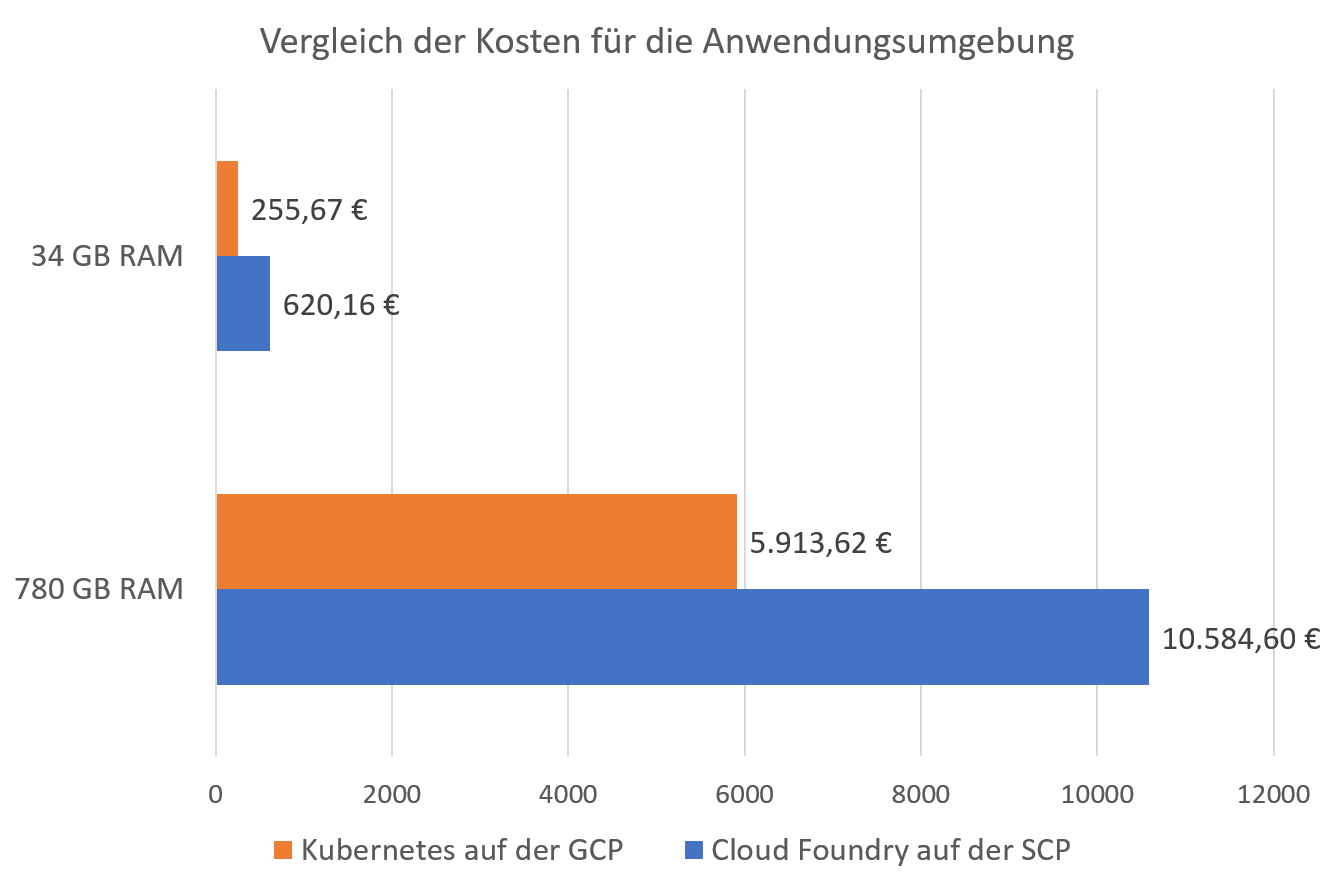
\includegraphics[width=14cm]{img/Kostenvergleich.png}
		\caption[Kostenvergleich Anwendungsumgebung für \acs{CF} und Kubernetes]{Kostenvergleich Anwendungsumgebung für \acl{CF} und Kubernetes}
		\label{grafik_kostenvergleich}
	\end{center}
\end{figure}
\\
Des Weiteren erfolgt die generelle Kostenberechnung der \ac{GCP} ausschließlich auf den tatsächlich konsumierten Infrastrukturressourcen. Im Vergleich dazu werden innerhalb des SAP Subscription Billing Projektes die Gebühren der von der \ac{SCP} angebotenen \ac{CF}-Umgebung unabhängig von dem tatsächlichen Verbrauch berechnet. Hierbei fallen seitens der \ac{SCP} feste monatliche Kosten an.\\
Auch der Vergleich der Sicherheitskonzepte der beiden Plattformen hat gezeigt, dass durch das standardmäßige Nichtvorhandensein von extern verfügbaren Endpunkten keine zusätzlichen Sicherheitsvorkehrungen zur Absicherung der Schnittstellen benötigt werden. Zudem stellte sich die automatische Verwendung von \ac{mTLS} innerhalb des Kubernetes Clusters für die Absicherung der Kommunikation als sehr hilfreich heraus.\\
Da die Verfügbarkeit der beiden Plattformen hauptsächlich von der Verfügbarkeit des zugrundeliegenden \ac{IaaS}-Providers abhängig ist und zusätzlich weitere Abhängigkeiten, wie beispielsweise die Verfügbarkeit der verwendeten Datenbanken existieren, konnte kein klarer Unterschied bezüglich der Verfügbarkeit der beiden Plattformen festgestellt werden.\\
Allerdings zeichnet sich Kubernetes besonders durch die Möglichkeiten der dynamischen Skalierung aus. Hierbei unterstützt Kubernetes sowohl die automatische horizontale als auch vertikale Skalierung auf der Pod-Ebene oder auch die gesamte Skalierung der für das Cluster bereitgestellten Rechenressourcen des \ac{IaaS}-Providers.\\
Die \ac{CF} hingegen unterstützt mit Hilfe des App-Autoscaler-Projekt zwar die dynamische vertikale Skalierung einer Anwendung, jedoch kann die horizontale Skalierung ausschließlich manuell und nicht automatisiert durchgeführt werden.\\
Generell unterstützt Kubernetes durch die mögliche Konfiguration aller vorhandenen \ac{API}-Objekte sowie den zusätzlich angebotenen Custom Ressource Definitions eine sehr detaillierte Konfiguration des gesamten Kubernetes Clusters als auch der einzelnen Anwendungsbereitstellung. Durch die Verwendung des Service Meshes Istio können besonders im Bereich des Traffic Managements umfangreiche Konfigurationen von Funktionalitäten, wie beispielsweise dem gewichteten Routing der Anfragen, vorgenommen werden, welche bei der \ac{CF} gar nicht unterstützt werden. Außerdem zeigte die innerhalb des SAP Subscription Billing Projektes praktische Verwendung der \ac{CF}, dass aufgrund fehlender Konfigurationsmöglichkeiten Probleme bei dem produktiven Betrieb der Softwarelösung auftreten können. Ein Beispiel dafür ist die nicht konfigurierbare Timeoutzeit der Health Checks.\\
Im Punkt der Erweiterbarkeit bieten die beiden Plattformen mit dem Blue-Green Deployment der \ac{CF} und der Rolling Update Strategie von Kubernetes grundsätzlich sehr ähnliche Strategien für die Aktualisierung der bereitgestellten Anwendungen mit Zero-Downtime an. Generell unterstützt Kubernetes durch das sehr breite Spektrum an vorkonfigurierten Helm Charts die Erweiterung der Infrastrukturlösung um zusätzliche Open Source Tools mit minimalem Aufwand.\\
Die praktische Umsetzung des Kubernetes Prototyps hat gezeigt, dass das hierfür benötigte Vorwissen und die Einarbeitungszeit definitiv höher als bei der \ac{CF} ist, weshalb dies bei einer Portierung der gesamten Softwarelösung berücksichtigt und eingeplant werden sollte.\\
\\
Besonders mit Hilfe des nativ unterstützten Multi Zonen Konzeptes zeichnet sich Kubernetes im Punkt der Portierbarkeit aus. Dabei können Kubernetes Cluster, deren Infrastruktur auf unterschiedlichen \ac{IaaS}-Providern in mehreren Zonen bereitgestellt wird, konzeptioniert und umgesetzt werden. Dahingegen ist eine \ac{CF}-Space immer an eine Zone eines \ac{IaaS}-Providers gebunden. Somit kann die auf der \ac{CF} bereitgestellte Softwarelösung nicht ohne Umstände auf einen anderen \ac{IaaS}-Provider oder in eine andere Zone portiert werden.\\
Anhand der erfolgreichen Ersetzung einiger innerhalb der aktuellen Infrastrukturlösung zusätzlich benötigter Infrastruktur-Services und Komponenten durch native Funktionalitäten und Objekte von Kubernetes und Istio konnte gezeigt werden, dass Kubernetes in dem Vergleichsmerkmal Infrastruktur-Services definitiv vorteilhaft ist. \\
Insgesamt bietet die Kubernetes Plattform besonders in Kombination mit dem Service Mesh Istio bereits sehr viele Funktionalitäten nativ an, welche für den produktiven Betrieb eine Cloud nativen \ac{SaaS}-Lösung benötigt werden. Auch die teilweise innerhalb der Microservices implementierten Funktionalitäten, wie beispielsweise die gegenseitige Authentifizierung der Microservices, werden im Kubernetes Prototyp nicht mehr benötigt und von der Plattform selbst übernommen.\\
Im Punkt der Dienste für das Monitoring- und Logging-Konzept der bereitgestellten Anwendung bieten die von der \ac{SCP} angebotenen Dienste standardmäßige Möglichkeiten, welche keine weiteren Implementierungen oder einen eigenen Betrieb der Tools benötigen. Jedoch zeigte die mittels des Prototyps erfolgreich umgesetzte Implementierung der im SAP Subscription Billing Projekt eingesetzten Tools, dass diese auch für das Kubernetes Cluster implementiert und ohne Limitationen verwendet werden können. Allerdings muss hierbei der Betrieb des ELK Stacks und die Verwaltung und Archivierung der Logdateien selbst übernommen werden. Diese Aufgaben werden innerhalb der Dienste der \ac{SCP} zwar übernommen, jedoch fallen hierfür auch feste monatliche Servicegebühren an.\\
Außerdem konnten besonders durch den Einsatz des Service Meshes Istio zusätzliche Funktionalitäten umgesetzt werden, welche bisher in der aktuellen Infrastrukturlösung nicht möglich gewesen sind. Dazu gehört beispielsweise das Tool \textbf{Kiali}, welches als grafische Webanwendung für die Verwaltung und Steuerung der gesamten Netzwerkkommunikation genutzt werden kann. Ein Ausschnitt der grafischen Darstellung der Netzwerkkommunikation des Kiali Tools ist im Anhang in Abbildung \ref{anhang_kiali_dashboard} zu finden.\\
Des Weiteren implementiert Istio das Tracing Tool \textbf{Jaeger}. Dieses kann für die Nachvollziehbarkeit aufeinander folgender Anfragen verwendet werden. Für dessen Verwendung müssen ausschließlich weitere \ac{HTTP}-Header und die Funktionalität der Weitergabe der \ac{HTTP}-Header in die Microservices eingebaut werden. Eine Anleitung für die praktische Umsetzung der Weitergabe der \ac{HTTP}-Header ist unter dem angegebenen Link zu finden.\footnote{Anleitung Umsetzung Weitergabe \ac{HTTP}-Header: \url{https://istio.io/docs/tasks/observability/distributed-tracing/overview/\#trace-context-propagation}} Jedoch wurde dies aufgrund des beschränkten zeitlichen Rahmens der vorliegenden Thesis nicht umgesetzt und dient ausschließlich zum Aufzeigen weiterer möglichen Funktionalitäten des Service Meshes Istio.\\
\\
Anhand der zuvor zusammengefassten Ergebnisse der Evaluationen der beiden Plattformen sowie durch die erfolgreiche prototypische Portierung der SAP Subscription Billing Lösung auf das Kubernetes Cluster und der dabei umgesetzten Funktionalitäten und zusätzlichen Möglichkeiten kann die am Anfang der vorliegenden Thesis gestellte wissenschaftliche Fragestellung, ob der Einsatz einer containerbasierten Infrastrukturlösung für die Weiterentwicklung und den Betrieb der \ac{SaaS}-Lösung im Bezug zur bisherigen Infrastrukturlösung verbessert werden kann, mit einem ``Ja`` beantwortet werden.\\ 
Dieses Fazit begründet sich auch durch die in Kapitel \ref{gewichtung_merkmale} erläuterte Gewichtung der Merkmale. Dabei sind für das Infrastruktur-Team des Projektes die Merkmale Sicherheit, Verfügbarkeit, Skalierbarkeit, Konfigurierbarkeit, Erweiterbarkeit und Monitoring und Logging für die Begründung der Entscheidung einer Plattform ausschlaggebend. Besonders die Konfigurierbarkeit und Sicherheit der Bereitstellung der \ac{SaaS}-Lösung kann durch die zuvor zusammengefassten Funktionalitäten von Kubernetes und Istio verbessert werden. Generell kann durch das Ersetzen einiger zusätzlicher Infrastruktur-Services und Komponenten insgesamt die Komplexität der Infrastrukturlösung und somit auch der Wartungsaufwand verringert werden.\\ 
Ausschließlich innerhalb der Möglichkeiten für das Management der Logdateien der bereitgestellten Anwendungen existiert für Kubernetes kein standardmäßiges ``as-a-Service``-Angebot, weshalb der ELK-Stack einmalig selbst implementiert und betrieben werden muss. Da dies innerhalb der ausschlaggebenden Merkmale des Infrastruktur-Teams allerdings der einzige Nachteil bei der Verwendung von Kubernetes ist, kann dieser, verglichen mit den umfangreichen Möglichkeiten und den Vorteilen von Kubernetes, vernachlässigt werden und sollte ausschließlich in der Planung der finalen Portierung der \ac{SaaS}-Lösung dementsprechend berücksichtigt werden.\\
\\
Bezüglich der kritischen Reflexion der Ergebnisse der vorliegenden Thesis sollte beachtet werden, dass innerhalb der prototypischen Portierung der \ac{SaaS}-Lösung eine repräsentative Auswahl an Microservices verwendet wurde. Dadurch kann nicht ausgeschlossen werden, dass bei einer Portierung der gesamten Infrastrukturlösung bisher nicht vorhandene Herausforderungen entstehen.\\
Außerdem ist zu berücksichtigen, dass für den Prototyp lokale Instanzen der benötigten Datenbanken auf dem Cluster selbst bereitgestellt wurden. Allerdings werden in der aktuellen Infrastrukturlösung die von der \ac{SCP} angebotenen Dienste für die Bereitstellung und den Betrieb der Datenbanken verwendet. Deshalb sollte für die produktive Portierung entweder eine Integration der gemanagten Datenbanken der \ac{SCP} oder ein Konzept zur eigenen Bereitstellung und Verwaltung der Datenbanken erstellt werden.\\
Zwar wurden aufgrund des Faktes, dass das Kubernetes Cluster ausschließlich für den Prototyp provisioniert und vom Autor der vorliegenden Thesis verwendet wurde, kein Berechtigungskonzept für den Zugriff auf das Kubernetes Cluster benötigt. Allerdings sollte dies bei einer produktiven Verwendung definitiv mit dem in Kapitel \ref{bewertung_k8s_prototyp} erläuterten Sicherheitskonzept für die Absicherung des externen Zugriffs auf das Kubernetes Cluster umgesetzt werden.\\
Des Weiteren basiert der Kostenvergleich der beiden Plattformen ausschließlich auf den für die Application Runtime Umgebung anfallenden Kosten. Hierbei sollte jedoch für einen umfangreichen und repräsentativen Kostenvergleich die Betrachtung der gesamten \ac{TCO} durchgeführt werden.
 
\newpage
\section{Ausblick Infrastrukturlösung SAP Subscription Billing}
\label{ausblick}
Die vorliegende Thesis hat gezeigt, dass die Portierung der SAP Subscription Billing Lösung auf ein Kubernetes Cluster definitiv als sinnvoll betrachtet werden kann. Dies wurde auch bei der Präsentation der Ergebnisse innerhalb des Infrastruktur-Teams des Projektes anerkannt und bestätigt.\\
Jedoch ist besonders die komplette Portierung der \ac{SaaS}-Lösung, insbesondere, da diese bereits bei einigen Kunden produktiv eingesetzt wird, realistisch betrachtet nicht in kurzer Zeit möglich und sollte umfangreich geplant und vorbereitet werden. Allerdings konnte mittels der vorliegenden Thesis erfolgreich bewiesen werden, dass dieser Aufwand durchaus sinnvoll ist.\\
Deshalb sieht der langfristige Plan des SAP Subscription Billing Projektes die schrittweise Portierung der Softwarelösung in ein Kubernetes Cluster vor. Hierbei dient die vorliegende Thesis als essentielle Grundlage, welche die theoretischen Konzepte der Kubernetes Plattform und dem Service Mesh Istio vorstellt sowie exemplarische Implementierungen für deren praktische Verwendung aufzeigt.\\
Ebenso wurde vom Autor der vorliegenden Thesis ein zusätzliches Konzept zur automatischen Portierung aller Microservices der \ac{SaaS}-Lösung erstellt. Dabei wurde eine eigenständige Jenkins-Pipeline implementiert, welche mit Hilfe von Skripts, einem eigens erstellten Helm Chart und dem Skaffold Tool die automatische Bereitstellung aller Microservices und den weiteren benötigten Objekten von Kubernetes und Istio auf das Kubernetes Cluster ermöglicht. Weitere Informationen zu der über den Rahmen der vorliegenden Thesis hinausgehende Umsetzung des zuvor genannten Konzeptes sind im Anhang in Kapitel \ref{anhang_umsetzung_komplettes_Deployment} zu finden.\\

\newpage
\section{Entwicklungsmöglichkeiten von \acs{SaaS}-Lösungen durch Kubernetes}
\label{Entwicklungsmöglichkeiten_Kubernetes_SaaS}
Besonders bei \ac{SaaS}-Lösungen, welche auf einer Microservice-Architektur basieren, existieren einige Herausforderungen, wie beispielsweise benötigte Funktionalitäten für Tracing, Traffic Management oder auch das Berechtigungs- und Sicherheitskonzept für einzelne Mandanten. Diese sind speziell im Cloud nativen Umfeld sehr relevant und prägen sich weiter bei einem weltweiten produktiven Einsatz der \ac{SaaS}-Lösung aus.\\
Um den dabei entstehenden Anforderungen besonders im Bereich der Verfügbarkeit und Skalierbarkeit der Software gerecht werden zu können, bietet Kubernetes grundlegende Mechanismen und Konzepte, wie zum Beispiel die automatische vertikale und horizontale Skalierung auf mehreren Ebenen sowie auch das Multi Zone Konzept für eine regional verteilte Bereitstellung der Softwarelösung, an. Auch die Vision des Cluster Federation Projektes, welches auf die virtuelle Aggregation heterogen bereitgestellter Kubernetes Cluster abzielt, wird mit großer Wahrscheinlichkeit in naher Zukunft sehr relevant werden und eröffnet beispielsweise für einen hybriden Cloudansatz neue Möglichkeiten.\\ 
Dabei können exemplarisch Teile der Softwarelösung, welche aus bestimmten Sicherheitsaspekten besonders geschützt werden müssen, auf einem privaten Cluster, das in eigenen Rechenzentren des Kunden betrieben wird, bereitgestellt werden. Wohingegen die Teile der Softwarelösung, welche eine dynamische und globale Skalierbarkeit benötigen, in einem Public-Cloud Cluster des \ac{SaaS}-Anbieters bereitgestellt werden können. Dieses könnte mittels des Multi Zone Konzeptes auf der Infrastruktur unterschiedlicher \ac{IaaS}-Provider aus regional verteilten Zonen basieren, um die Abhängigkeit eines einzelnen Rechenzentrums des \ac{IaaS}-Providers zu umgehen.\\
Somit unterstützt Kubernetes optimal die Entwicklung und den Betrieb von Cloud nativen \ac{SaaS}-Lösungen. Dadurch rechtfertigt Kubernetes seinen aktuellen Status als Industriestandard für die Orchestration von Containeranwendung und hat mit den geplanten Weiterentwicklungen durchaus Potenzial, diesen Status auch in der Zukunft weiter ausbauen zu können. 



% Der Anhang beginnt hier - jedes Kapitel wird alphabetisch aufgezählt. (Anhang A, B usw.)
\appendix
\ihead{\appendixname~\thechapter} % Neue Header-Definition
%\pagenumbering{gobble}
\cleardoublepage
\pagenumbering{roman} % Römische Seitennummerierung
\setcounter{page}{7}
\chapter{Anhang}
\section{Technischer Aufbau SAP Subscription Billing}
\label{anhang_cf_infrastruktur}
\begin{figure}[h]
	\begin{center}
		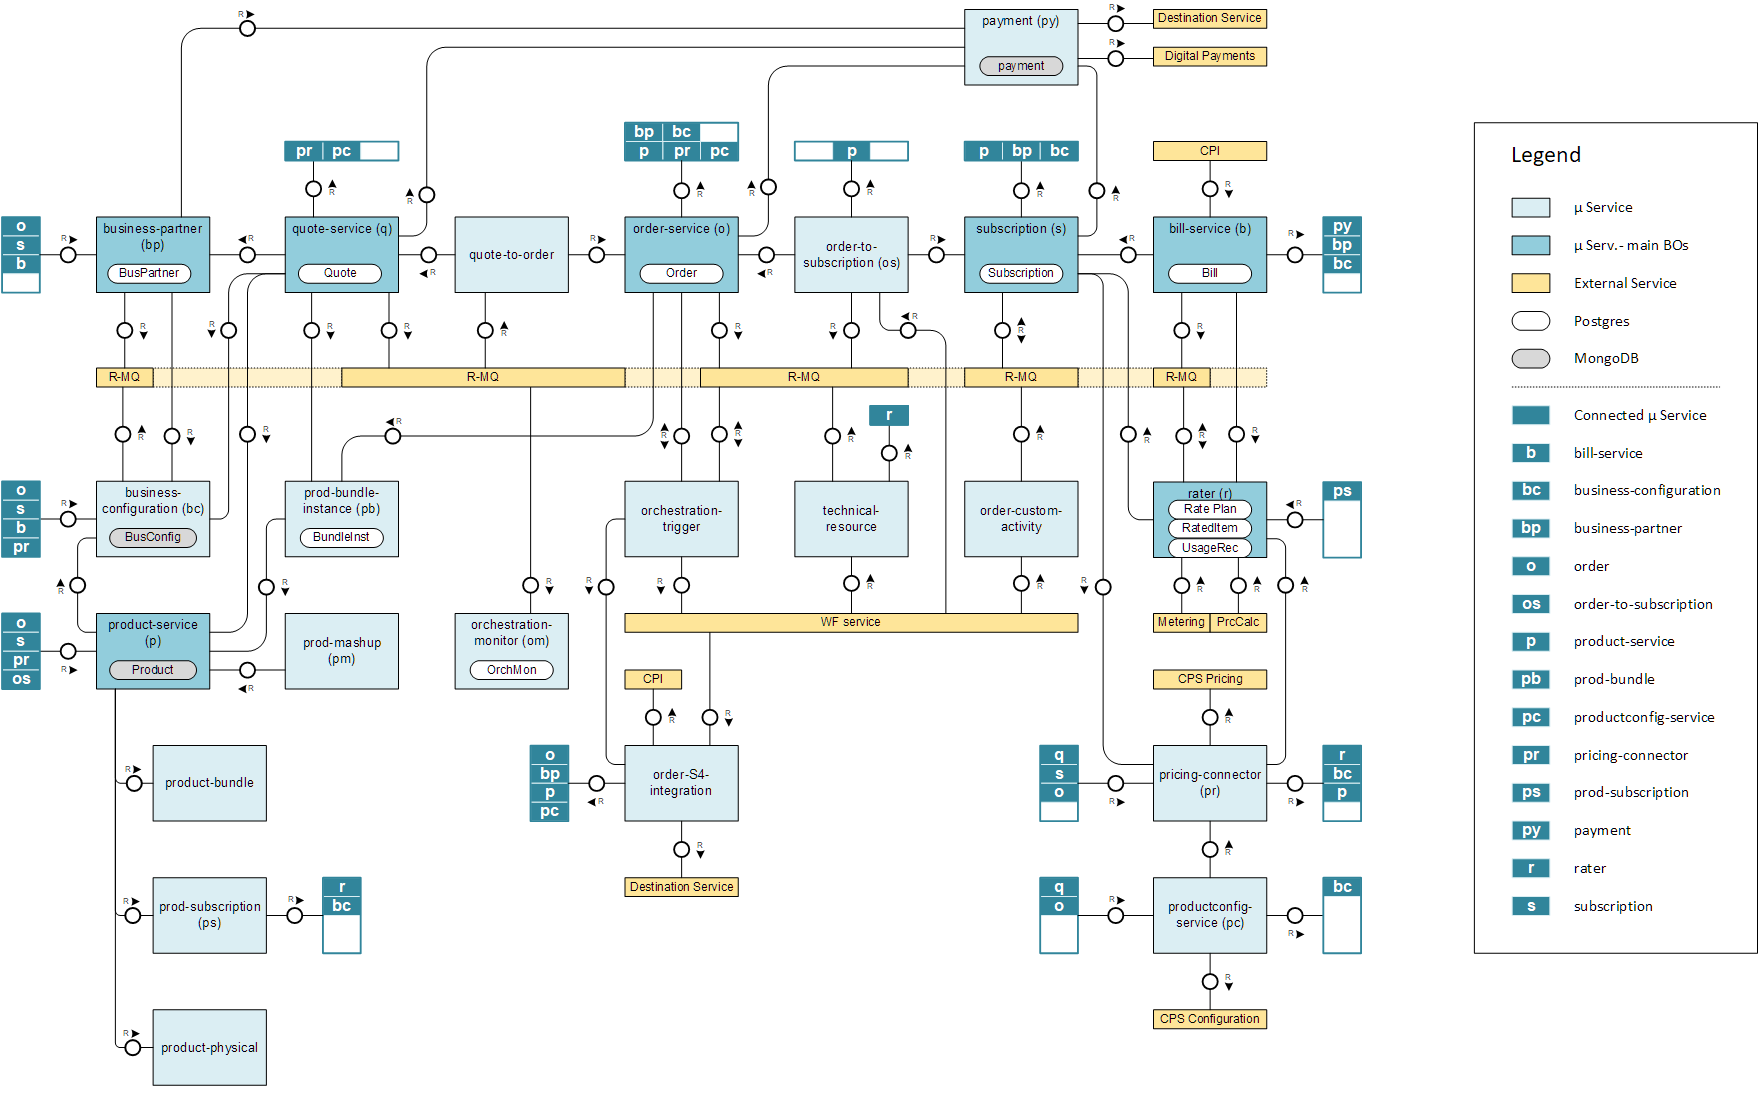
\includegraphics[width=16cm]{img/ssb_microservices.JPG}
		\caption[Technischer Überblick Microservices und Datenbanken der SAP Subschription Billing Softwarelösung]{Technischer Überblick Microservices und Datenbanken der SAP Subschription Billing Softwarelösung\\ (Abbildung stammt aus dem projektinternen Wiki)}
		\label{grafik_ssb_microservices}
	\end{center}
\end{figure}

\newpage
\section{Untersuchung der Performance mittels JMeter}
\subsection{Testsetup für die Messung der Performance}
\label{anhang_performancetests}
Bei der Messung der Performance wurde folgende \ac{HTTPS}-Anfrage an den Endpunkt des Rater-Microservices gesendet. Dabei wurden die jeweiligen extern verfügbaren \acsp{URL} für den Zugriff auf den Rater-Microservice verwendet.\\
\begin{enumerate}
	\item \ac{CF}: \url{https://rater.cfapps.eu10.hana.ondemand.com}
	\item Gardener Kubernetes Cluster: \url{rater.ingress.k8s-sb.subbilling.shoot.canary.k8s-hana.ondemand.com}
	\item Converged Cloud Kubernetes Cluster: \url{https://rater.subscription-billing.c.eu-de-2.cloud.sap}
\end{enumerate}
Es wurde jeweils eine \ac{HTTPS}-POST Anfrage an den folgenden Pfad  mit dem im Quelltext \ref{quellcode_anfrage_performancetests} dargestellten Bodyinhalt gesendet: \textbf{/estimation/public/v1/estimation}\\
Jedoch ist zu beachten, dass hierfür eine erfolgreiche Authentifikation und Autorisierung mittels mehrerer \ac{HTTP}-Header benötigt wird. Es ist zu beachten, dass die angegeben Adressen zwar extern verfügbar sind, jedoch ausschließlich mit einer erfolgreichen Authentifizierung mittels OAuth 2.0 erreichbar sind.\\
Insgesamt wurde jedes Testsetup jeweils mit fünf Testläufen ausgeführt. Dabei betrug das Testintervall der durchgeführten Tests jeweils fünf Minuten pro Testlauf. Dabei wurde jeweils mit 100, 150 und 200 parallelen Threads getestet, welche gleichzeitig zuvor dargestellte \ac{HTTPS}-Anfrage senden.
\newpage
\begin{lstlisting}[language=yaml, caption=Verwendete \acl{HTTPS}-Anfrage für die Messung der Performance, label=quellcode_anfrage_performancetests]
{
	"ratePlans": [
		{
			"id": "${__UUID()}",
			"fixedRates": [
				{
					"id": "${__UUID()}",
					"price": {
						"amount": 5.09,
						"currency": "EUR"
					},
					"metricId": "FIXED_RATE_METRIC_ID",
					"billedInAdvance": false
				}
			],
			"blockRates": [
				{
					"id": "${__UUID()}",
					"pricePerBlock": {
						"amount": 19.81,
						"currency": "EUR"
				},
				"blockSize": 100,
				"metricId": "API_CALL"
				}
			]
		}
	],
	"usageEstimates": [
		{
			"metricId": "API_CALL",
			"quantity": ${__Random(0,1000)}
		}
	]
}
\end{lstlisting}
\newpage
\subsection{Ergebnisse der Performancetests der beiden Plattformen}
\label{section_performance_test}
\subsubsection{Cloud Foundry Umgebung in Frankfurt}
\label{section_performance_test_cf}
\begin{figure}[h]
	\begin{center}
		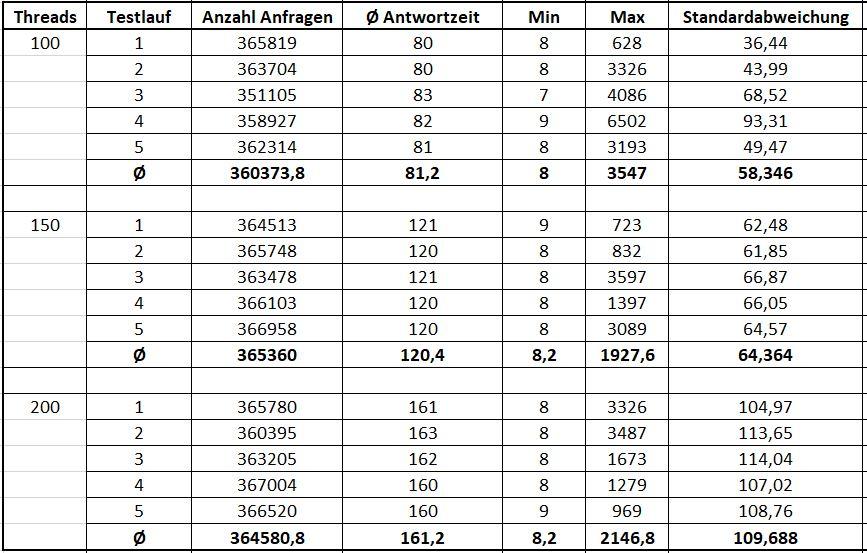
\includegraphics[width=16cm]{img/performance_cf_1.JPG}
		\caption[Performancetests: Cloud Foundry Teil 1]{Ergebnisse Performancetests: Cloud Foundry Teil 1}
		\label{performance_cf_1}
	\end{center}
\end{figure}
\newpage
\begin{figure}[h]
	\begin{center}
		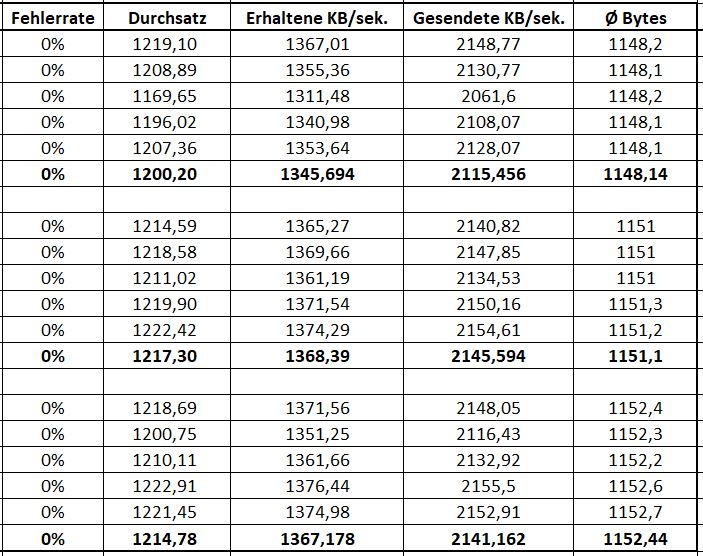
\includegraphics[width=16cm]{img/performance_cf_2.JPG}
		\caption[Performancetests: Cloud Foundry Teil 2]{Ergebnisse Performancetests: Cloud Foundry Teil 2}
		\label{performance_cf_2}
	\end{center}
\end{figure}
\newpage
\subsubsection{Gardener Kubernetes Cluster in Belgien}
\label{section_performance_k8s_gardener}
\begin{figure}[h]
	\begin{center}
		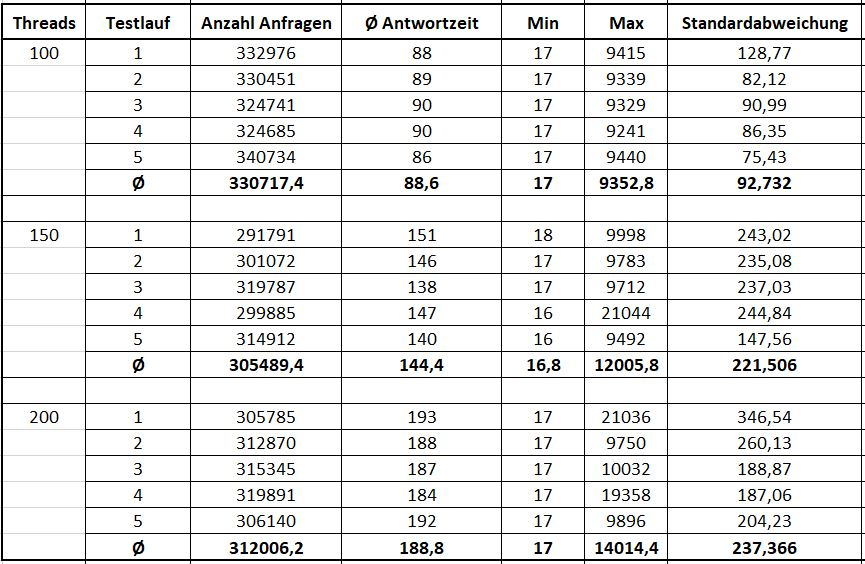
\includegraphics[width=16cm]{img/performance_k8s_1.JPG}
		\caption[Performancetests: Gardener Kubernetes Cluster Teil 1]{Ergebnisse Performancetests: Gardener Kubernetes Cluster Teil 1}
		\label{performance_k8s_1}
	\end{center}
\end{figure}
\newpage
\begin{figure}[h]
	\begin{center}
		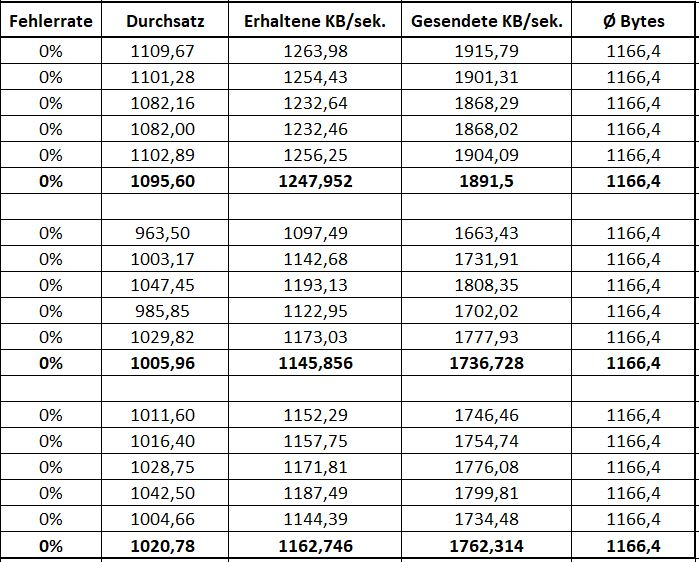
\includegraphics[width=16cm]{img/performance_k8s_2.JPG}
		\caption[Performancetests: Gardener Kubernetes Cluster Teil 2]{Ergebnisse Performancetests: Gardener Kubernetes Cluster Teil 2}
		\label{performance_k8s_2}
	\end{center}
\end{figure}
\newpage
\subsubsection{Converged Cloud Kubernetes Cluster in Frankfurt}
\label{section_performance_k8s_con_cloud}
\begin{figure}[h]
	\begin{center}
		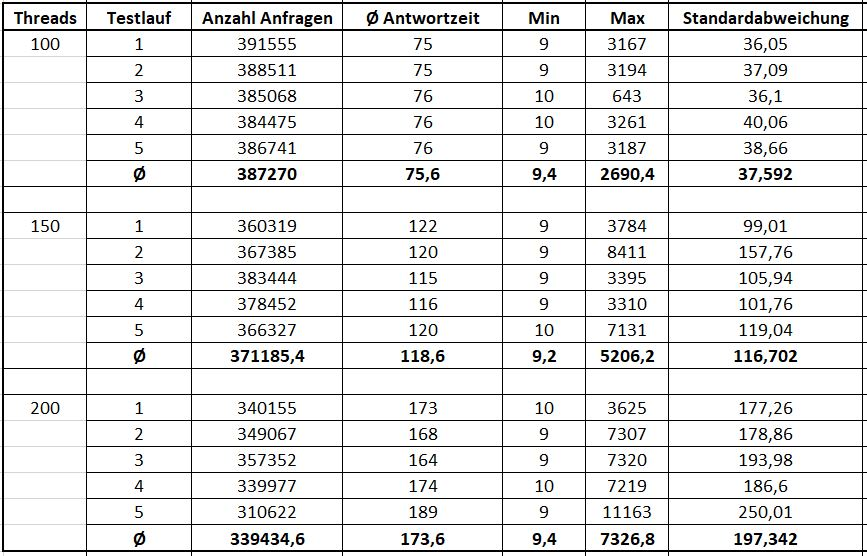
\includegraphics[width=16cm]{img/performance_con_cloud_1.JPG}
		\caption[Performancetests: Converged Cloud Kubernetes Cluster Teil 1]{Ergebnisse Performancetests: Converged Cloud Kubernetes Cluster Teil 1}
		\label{performance_con_cloud_1}
	\end{center}
\end{figure}
\newpage
\begin{figure}[h]
	\begin{center}
		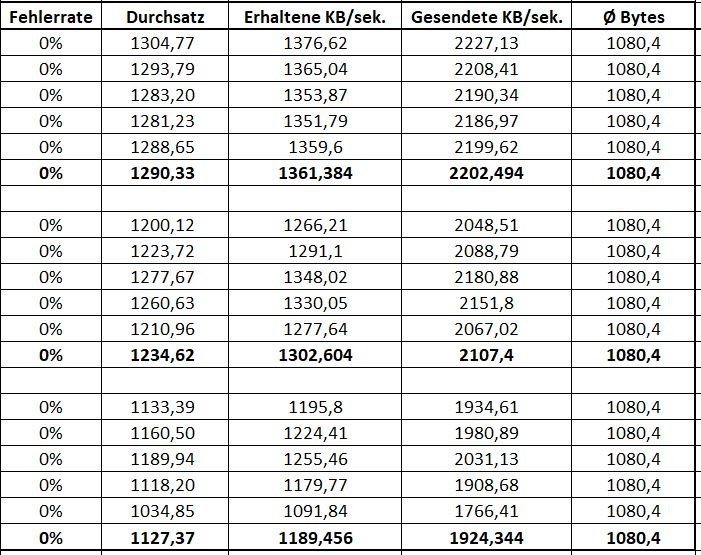
\includegraphics[width=16cm]{img/performance_con_cloud_2.JPG}
		\caption[Performancetests: Converged Cloud Kubernetes Cluster Teil 2]{Ergebnisse Performancetests: Converged Cloud Kubernetes Cluster Teil 2}
		\label{performance_con_cloud_2}
	\end{center}
\end{figure}

\newpage

\section{Beispielhafte Manifestdateien und Quellcode}
\subsection{Bereitstellung der Microservices}
\begin{lstlisting}[language=yaml, caption=Dockerfile des Rater-Microservices, label=quellcode_bereitstellung_microservices]
FROM openjdk: 8-jdk-alpine
ADD /target/rating-rater-0.48.0-SNAPSHOT-exec.jar app.jar
ENTRYPOINT ["java","-Djava.security.egd=file:/dev/./urandom","-jar","/app.jar"]
\end{lstlisting}
Für die Bereistellung der Microservices wird das Open Source Java Development Kit \textbf{OpenJDK} verwendet.\footnote{Offizielles OpenJDK Docker-Image: \url{https://hub.docker.com/_/openjdk}}
Zudem wird die ausführbare \textbf{app.jar}-Datei in den Container kopiert. Diese wird nach erfolgreichem Start des Containers von der lokalen Java Runtime ausgeführt. Das hierfür verwendete Kommando ist der dritten Zeile des zuvor dargestellten Dockerfiles zu entnehmen.\\
\\
Aus den folgenden Quelltexten sind beispielhafte Manifestdateien, welche für die Bereitstellung der Microservices implementiert worden sind. Diese können theoretisch für jedes beliebiges Kubernetes Cluster wiederverwendet werden. Allerdings wird hierfür der in den Manifestdateien definierte Namespace \textbf{dev} sowie die Secrets und die Config Maps benötigt. Aus Sicherheitsgründen kann das Secret für den Zugriff auf die SAP eigene Docker Registry nicht innerhalb der vorliegenden Thesis inkludiert werden.
\\
\lstinputlisting[language=yaml, caption=Beispielhafte Manifestdatei für das Stateful Set des Rater-Microservice, label=quellcode_statefulset_rater]{quellcode/rater.statefulset.yaml}
\newpage
\lstinputlisting[language=yaml, caption=Beispielhafte Manifestdatei für den Horizontal Pod Autoscaler des Rater-Microservices, label=quellcode_hpa_rater]{quellcode/rater.hpa.yaml}
\lstinputlisting[language=yaml, caption=Beispielhafte Manifestdatei für die Config Map des Rater-Microservices, label=quellcode_cm_rater]{quellcode/rater.configmap.yaml}
\newpage
\lstinputlisting[language=yaml, caption=Beispielhafte Manifestdatei für das Stateful Set der MongoDB-Instanz für den Business-Config-Microservice, label=quellcode_statefulset_mongodb]{quellcode/mongodb.statefulset.yaml}
\newpage
\lstinputlisting[language=yaml, caption=Beispielhafte Manifestdatei der \acl{GCP} spezifischen Storage Class zur persistenten Speicherung der Daten, label=quellcode_storageclass_gcp]{quellcode/mongodb.statefulset.yaml}
\newpage
\subsection{Verschiedene Landschaften}
\label{quellcode_verschiedene_landschaften}
\lstinputlisting[language=yaml, caption=Beispielhafte Manifestdatei für den Namespace dev, label=quellcode_namespaces]{quellcode/namespaces.yaml}
\lstinputlisting[language=yaml, caption=Beispielhafte Manifestdatei für den Ingress Service, label=quellcode_ingress_service]{quellcode/global.ingress.yaml}
\newpage
\lstinputlisting[language=yaml, caption=Beispielhafte Manifestdatei für das Default Gateway von Istio, label=quellcode_default_gateway]{quellcode/global.istio.gateway.yaml}
\lstinputlisting[language=yaml, caption=Beispielhafte Manifestdatei für die Destination Rule des Rater-Microservices, label=quellcode_routing_dr]{quellcode/rater.destinationrule.yaml}
\newpage
\lstinputlisting[language=yaml, caption=Beispielhafte Manifestdatei für den für das Routing der externen Anfragen verwendeten Virtual Service, label=quellcode_routing_vs]{quellcode/routing.virtualservice.ext.yaml}
\lstinputlisting[language=yaml, caption=Beispielhafte Manifestdatei für den Service der externen Anfragen des Rater-Microservices, label=quellcode_ext_service_rater]{quellcode/rater.service.ext.yaml}
\newpage
\lstinputlisting[language=yaml, caption=Network Policy für den Business-Config-Microservice, label=quellcode_business-config_np]{quellcode/business-config.networkpolicy.yaml}
\newpage
\subsection{Integration in die \acs{CI}/\acs{CD}-Pipeline}
\lstinputlisting[language=yaml, caption=Manifestdatei für das Skaffold Tool, label=quellcode_skaffold_rater]{quellcode/skaffold.yaml}
\newpage
\begin{lstlisting}[language=yaml, caption=Erweiterung Jenkinsfile um K8s Deployment Stage, label=quellcode_rater_jenkinsfile]
	@Library('ngom-modules')
	import com.sap.billcrowd.jenkins.execution.*
	import com.sap.billcrowd.jenkins.model.*
	
	node {
		try {
			k8sDeployment()
		} 
		catch (Exception e) {
			currentBuild.result = 'FAILURE'
			new BuildStatusEmail(this).sendEmail(e)
			throw e
		} 
		finally {
			deleteDir()
		}
	
	}
	
	def k8sDeployment() {
		try {
			PipelineUtil.sbDockerBuildTools(this, {
				stage("K8s Deployment") {
					container("skaffold") {
						unstash "dir"
						sh "skaffold run"
					}
				}
			})
		} catch (Exception e) {}
	}
\end{lstlisting}
\newpage
\subsection{Service-to-Service Kommunikation}
\label{anhang_s2s_kommunikation}
\lstinputlisting[language=yaml, caption=Beispielhafte Manifestdatei für den Service des Rater-Microservices, label=quellcode_rater_service]{quellcode/rater.service.yaml}
\newpage
\lstinputlisting[language=yaml, caption=Beispielhafte Manifestdatei für den Virtual Service des Rater-Microservices, label=quellcode_rater_vs]{quellcode/rater.virtualservice.yaml}
\lstinputlisting[language=yaml, caption=Globale \acl{mTLS}-Policy für den Istio Service Mesh, label=quellcode_globale_mtls_policy]{quellcode/global.mtlspolicy.yaml}

\clearpage

\section{Monitoring und Logging des Prototyps}
\begin{figure}[h]
	\begin{center}
		\includegraphics[width=16cm]{img/kibana_logs.PNG}
		\caption[Überblick Kibana Dashboard für Logs von Business-Config Microservice]{Überblick Kibana Dashboard für Logs von Business-Config Microservice}
		\label{anhang_grafik_kibana_dashboard}
	\end{center}
\end{figure}
\begin{figure}[h]
\begin{center}
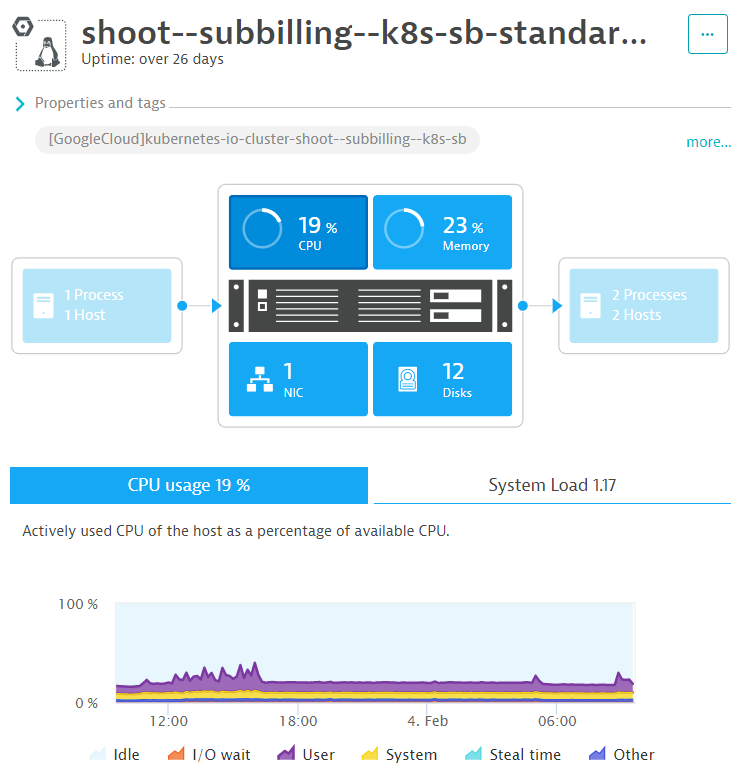
\includegraphics[width=16cm]{img/Dynatrace_Node_Monitoring.PNG}
\caption[Übersicht Dynatrace Dashboard für Monitoring einer Worker Node]{Übersicht Dynatrace Dashboard für Monitoring einer Worker Node}
\label{anhang_grafik_dynatrace_dashboard}
\end{center}
\end{figure}

\clearpage

\section{Zusätzliche Funktionalitäten des Kubernetes Protoyps}
\subsection{Kiali Tool für die Steuerung der Netzwerkkommunikation}
\begin{figure}[h]
	\begin{center}
		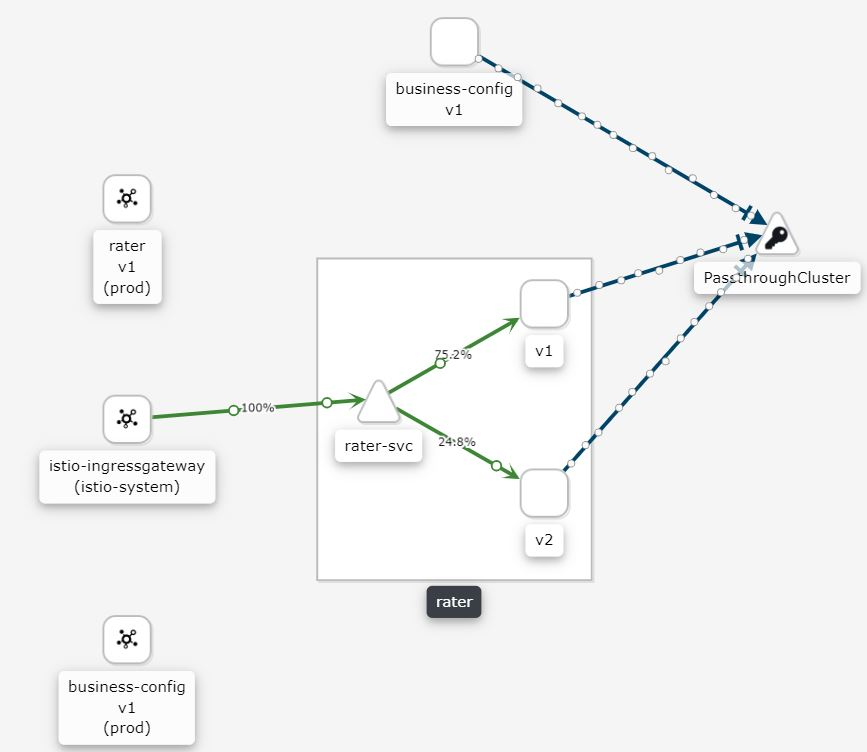
\includegraphics[width=16cm]{img/kiali_dashboard.JPG}
		\caption[Übersicht Routing externer Anfragen mittels Kiali Graphenansicht]{Übersicht Routing externer Anfragen mittels Kiali Graphenansicht}
		\label{anhang_kiali_dashboard}
	\end{center}
\end{figure}
\newpage
\begin{figure}[h]
	\begin{center}
		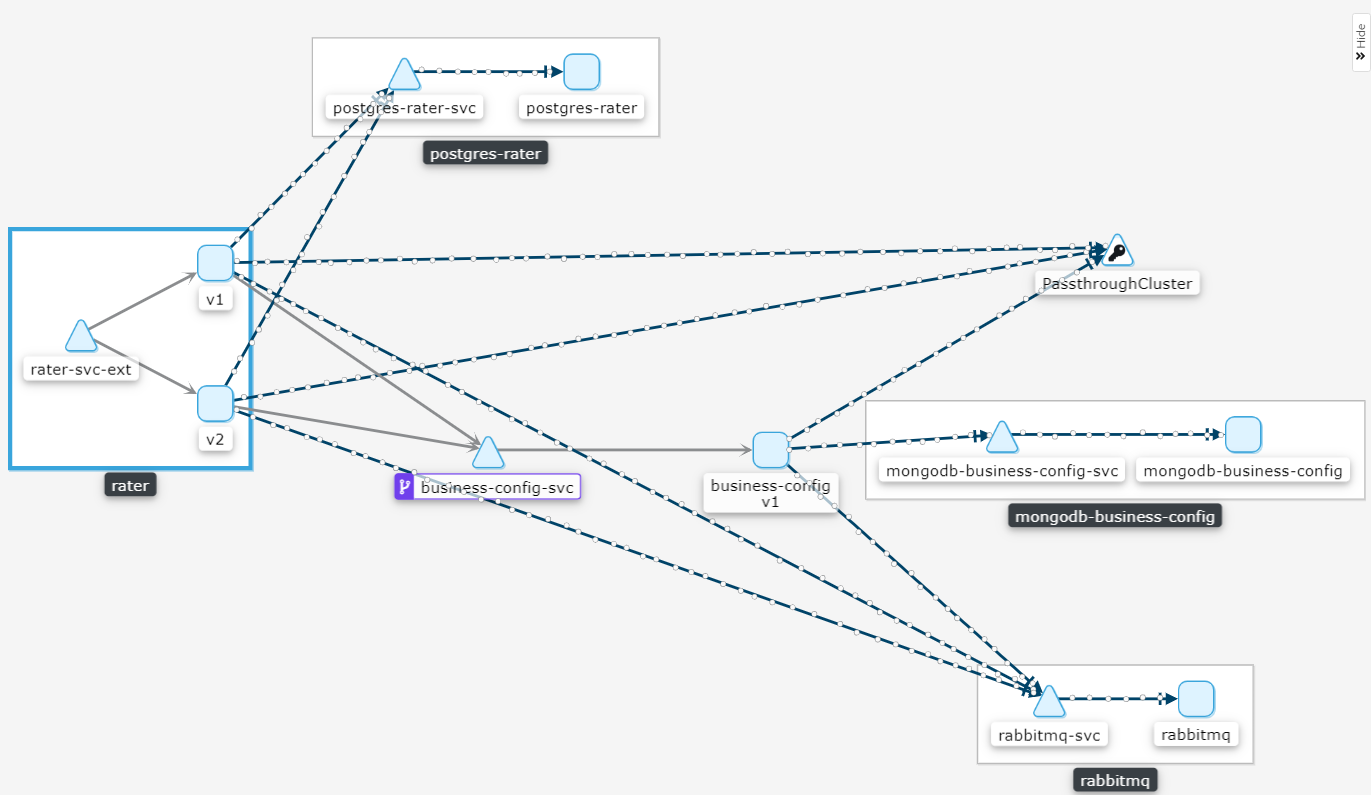
\includegraphics[width=16cm]{img/kiali_dashboard_2.PNG}
		\caption[Übersicht Netzwerkkommunikation mittels Kiali Graphenansicht]{Übersicht Netzwerkkommunikation mittels Kiali Graphenansicht}
		\label{anhang_kiali_dashboard}
	\end{center}
\end{figure}

\newpage

\subsection{Konzept zur Bereitstellung aller Microservices}
\label{anhang_umsetzung_komplettes_Deployment}
Wie in Kapitel \ref{ausblick} erwähnt wurde ein über den Rahmen der vorliegenden Thesis hinausgehendes Konzept für die automatische Bereitstellung aller Microservices der SAP Subscription Billing Lösung entwickelt und prototypisch umgesetzt.\\
Dabei sollte mit Hilfe eines Groovy Skriptes die vollständige Bereitstellung aller Microservices, welche in einem Vektor hinterlegt sind, in einem extra dafür neu angelegten Namespace auf dem Kubernetes Cluster bereitgestellt werden. Dabei ist zu erwähnen, dass auch der Namespace und alle weiteren benötigten Kubernetes-Objekte innerhalb des Prozesses automatisch neu erstellt werden.\\
Ziel des Konzeptes und des Prototyps ist die exemplarische Bereitstellung der Microservices in der im Vektor hinterlegten Version. Dadurch soll jede in der Vergangenheit vorgekommene Konstellation an Microservices in der richtigen Version nachgestellt werden können.\\
Die generellen Schritte des Skriptes sind der Abbildung \ref{anhang_k8s_vector_deployments} zu entnehmen.
\begin{figure}[h]
	\begin{center}
		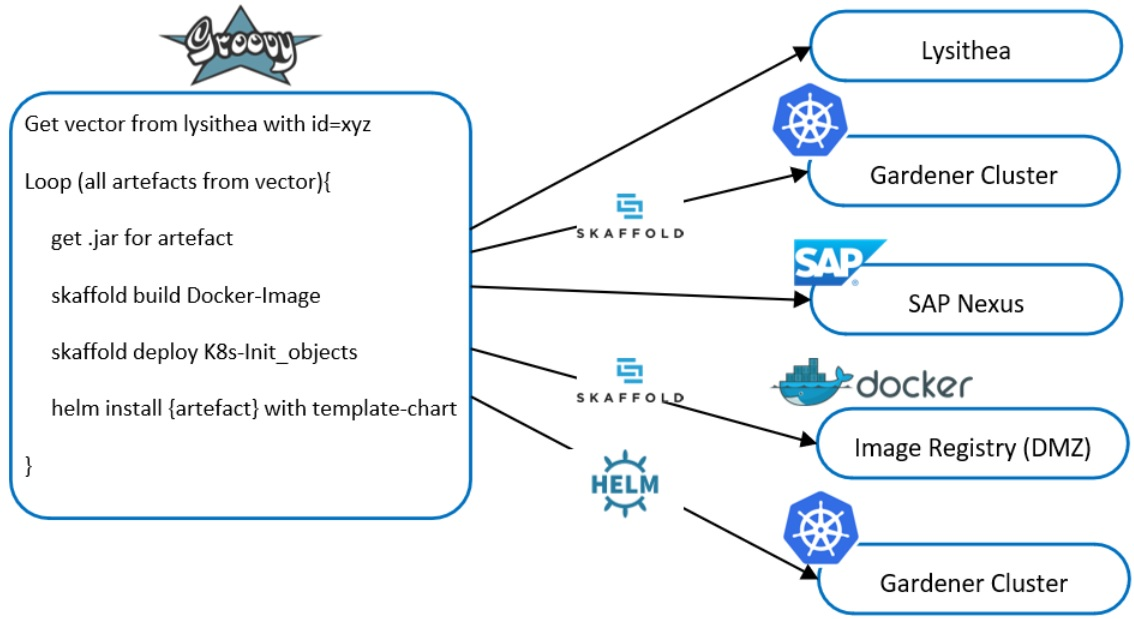
\includegraphics[width=16cm]{img/k8s_vector_deployment.JPG}
		\caption[Übersicht Funktionsweise automatisierten Bereitstellung aller Microservices]{Übersicht Funktionsweise automatisierten Bereitstellung aller Microservices}
		\label{anhang_k8s_vector_deployments}
	\end{center}
\end{figure}
Dabei wird innerhalb des Skriptes die aktuell noch manuell eingegebene ID des Vektors verwendet, um alle Informationen des Vektors und dessen Inhalt aus dem Lysithea-Service anfragen zu können.\\
Anschließend erfolgt mit Hilfe des Skaffold Tools die initiale Installation des Kubernetes Namespaces und der Secrets.\\
Danach beginnt eine Schleife, welche über alle Microservice-Artefakte des Vektors looped. 
Dabei wird für jedes Artefakt die folgenden Schritte durchgeführt:
\begin{enumerate}
	\item Herunterladen des Microservice Artefaktes aus dem SAP Nexus Repository
	\item Bauen des Docker-Images mit Hilfe der lokalen Docker Runtime
	\item Kennzeichnen des Docker-Images mittels der Version des Artefaktes
	\item Hochladen des Docker-Images auf die extern verfügbare Docker Registry von SAP
	\item Automatische Bereitstellung des Microservices mit Hilfe der Helm \ac{CLI} und der des eigens dafür erstellten Helm Charts auf das Kubernetes Cluster
\end{enumerate}
Hierbei ist zu erwähnen, dass mit Hilfe des eigens erstellten Helm Charts generelle Template Manifestdateien für alle benötigten \ac{API}-Objekte von Kubernetes und Istio definiert wurden.\\
Eine beispielhaftes Helm Template, welches für die Definition eines Stateful Sets zur Bereitstellung des eigentlichen Microservices verwendet wird, ist aus dem Quelltext \ref{quellcode_helm_template_ss} zu entnehmen. Ein weiteres Helm Template für die Bereitstellung der Virtual Services je Microservice ist in dem Quelltext \ref{quellcode_helm_template_vs} zu finden.
\\
\lstinputlisting[language=yaml, caption=Beispielhafte Manifestdatei des Helm Templates für das Stateful des Rater-Microservices, label=quellcode_helm_template_ss]{quellcode/microservice.statefulset.yaml}
\newpage
\lstinputlisting[language=yaml, caption=Beispielhafte Manifestdatei des Helm Templates für die Virtual Services der  Microservices, label=quellcode_helm_template_vs]{quellcode/microservice.virtualservice.yaml}

%	Literaturverzeichnis

\ihead{} % Neue Header-Definition
\cleardoublepage
%\pagenumbering{roman} % Römische Seitennummerierung
%\setcounter{page}{7}
\printbibliography[title=Literaturverzeichnis]
%\end{description}
% Ehrenwörtliche Erklärung ewerkl.tex einziehen
% !TEX root =  master.tex

\clearpage
\chapter*{Ehrenwörtliche Erklärung}

% Wird die folgende Zeile auskommentiert, erscheint die ehrenwörtliche
% Erklärung im Inhaltsverzeichnis.

% \addcontentsline{toc}{chapter}{Ehrenwörtliche Erklärung}
Ich versichere hiermit, dass ich die vorliegende Arbeit
 mit dem Thema: \textit{\DerTitelDerArbeit} selbstständig verfasst und keine anderen als die angegebenen Quellen und
Hilfsmittel benutzt habe. Ich versichere zudem,
dass die eingereichte elektronische Fassung mit der gedruckten Fassung übereinstimmt.

\vspace{3cm}
Ort, Datum \hfill \DerAutorDerArbeit



\end{document}
